% Лекции Сергея Борисовича Стечкина
% Версия 07.06.10 (ИММ)
% Версия 03.05.2020 -- подготовка второго издания

\documentclass{report}

\usepackage{stechkin}

%\title{ {\Huge {\bf Изложение лекций С.\,Б.\,Стечкина \\ по теории приближений}}}
%\author{{\bf С.\,Б.\,Стечкин}}
%\date{ }

\begin{document}


\thispagestyle{empty}
\begin{center}
{\footnotesize{\textbf{РОССИЙСКАЯ\ АКАДЕМИЯ\ НАУК}}}\\
{\footnotesize{\textbf{УРАЛЬСКОЕ\ ОТДЕЛЕНИЕ}}}\\
{\footnotesize{\textbf{ИНСТИТУТ\ МАТЕМАТИКИ\ И\
МЕХАНИКИ}}}\\
{\footnotesize{\textbf{МИНИСТЕРСТВО ОБРАЗОВАНИЯ И НАУКИ РФ}}}\\
{\footnotesize{\textbf{МОСКОВСКИЙ ГОСУДАРСТВЕННЫЙ УНИВЕРСИТЕТ ИМ. М.\,В.\,ЛОМОНОСОВА}}}
\\
{\footnotesize{\textbf{УРАЛЬСКИЙ ГОСУДАРСТВЕННЫЙ УНИВЕРСИТЕТ ИМ. А.\,М.\,ГОРЬКОГО}}}
\end{center}

\vspace{3cm}

\begin{center}
{\Huge{\textbf{ИЗЛОЖЕНИЕ ЛЕКЦИЙ \\ [5pt] С.\,Б.\,СТЕЧКИНА \\ [5pt] ПО ТЕОРИИ ПРИБЛИЖЕНИЙ \\[4pt]
               %: НАУЧНОЕ ИЗДАНИЕ\\[4pt]
                }}}
\end{center}

\vfill

\begin{center}
{\footnotesize{\textbf{ЕКАТЕРИНБУРГ,\ \ }}}\ {\footnotesize{\textbf{2010}}}
\end{center}

\newpage







\newpage
\thispagestyle{empty}


\vfill


\setcounter{page}{2}



%\large

\vspace*{1.5cm}

\noindent УДК\ 517.5
\hfill

\vspace{1cm}

\noindent{}\ \
{\textbf{Изложение лекций С.\,Б.\,Стечкина по теории приближений.}}\ \
Екатеринбург:\ УрО РАН,\ 2010. 154~c.\\[12pt]
ISBN~?--????--????--?

\vspace{5mm}

Материал книги -- результат обработки конспекта
лекций профессора С.\,Б.\,Стечкина по теории приближения,
прочитанных им как спецкурс на
механико-математическом факультете МГУ им.~М.\,В.\,Ло\-моносова в
1970--1971 учебном году. Спецкурсы С.\,Б.\,Стечкина, как и этот предлагаемый сейчас
читателю, отличались оригинальностью в выборе материала и
его изложении. Издание этого спецкурса будет
полезным и интересным как для студентов, так и для
преподавателей.

 \vspace{12mm}
\begin{center}
Редакционная коллегия: \\[2ex] {\em{член-корр. РАН}}
В.\,И.\,Бердышев (главный редактор); \\
 {\em{член-корр. РАН}} Ю.\,Н.\,Субботин;\\
{\em{доктор физ.-мат. наук }} В.\,В.\,Арестов;
{\em{доктор физ.-мат. наук }} С.\,В.\,Конягин; \\
{\em{доктор физ.-мат. наук }} С.\,А.\,Теляковский;
{\em{доктор физ.-мат. наук }} Н.\,Н.\,Холщевникова; \\
{\em{доктор физ.-мат. наук }} И.\,Г.\,Царьков; \\
{\em{доктор физ.-мат. наук }} Н.\,И.\,Черных (ответственный редактор); \\
{\em{доктор физ.-мат. наук }} В.\,А.\,Юдин.

 \end{center} \vfill


\noindent ISBN~???--?--????--????--?\\[12pt] Б\,$\frac{\textstyle
122(07)}{\textstyle 8\Pi 6(03)1998}$\,ПВ--2010\hfill
 $\copyright$\  ИММ УрО РАН,\ 2010~г.

\bigskip


%\begin{center}{\bf \Large Предисловие}\end{center}




\renewcommand{\chaptername}{Лекция}
%\renewcommand{\bibname}{Список литературы}
%\maketitle
\large
\sloppy

 \tableofcontents %%%% Содержание
 \begin{center}

{\Large \bf ПРЕДИСЛОВИЕ}

\end{center}

\ \

Настоящее издание возникло в результате обработки конспекта
лекций профессора С.\,Б.\,Стечкина по теории приближений, прочитанных им как спецкурс на
механико-математическом факультете МГУ им.~М.\,В.\,Ломоносова в
1970--1971 учебном году. Лекции были записаны студенткой
Т.\,В.\,Деминой.

Естественно, что такие студенческие записи
нуждались в доработке, которая была выполнена в последние
годы учениками С.\,Б.\,Стечкина. Лекции 1--4 к печати
готовил Ю.\,Н.\,Субботин, лекции 5--7 готовил С.\,А.\,Теляковский,
лекции 8--10 готовили В.\,И.\,Бердышев, Н.\,Н.\,Холщевникова и И.\,Г.\,Царьков,
лекции 11-13 готовили С.\,В.\,Конягин и И.\,Г.\,Царьков, лекции
14, 15 и частично 16 готовил В.\,А.\,Юдин, лекции 16--20
готовил В.\,В.\,Арестов.

Первоначальную обработку
оригинального конспекта лекций (расшифровка скорописи рукописного
текста, набор формул, исправление явных опечаток,
оформление рисунков) и последующую многократную перепечатку
материала лекций в процессе редактирования и согласования
осуществляли: в Москве -- А.\,И.\,Козко, Ю.\,В.\,Малыхин,
Т.\,В.\,Радославова, Н.\,Н.\,Холщевникова\footnote{Без инициативы и настойчивости
Натальи Николаевны эта книга вряд ли могла бы быть (прим. отв. редактора)};
в Екатеринбурге~--
П.\,Ю.\,Глазырина, М.\,В.\,Дейкалова, А.\,А.\,Кошелев,
Н.\,А.\,Куклин, К.\,С.\,Тихановцева, В.\,В.\,Шевченко.
Особенно большая работа легла на плечи М.\,В.\,Дейкаловой,
Ю.\,В.\,Малыхина, В.\,В.\,Шевченко.

Общее редактирование текста провел Н.\,И.\,Черных при большой поддержке и
помощи С.\,А.\,Теляковского, Н.\,Н.\,Холщевниковой и
Ю.\,В.\,Малыхина.

Различные варианты спецкурса по теории приближений
С.\,Б.\,Стечкин читал систематически, почти каждый учебный
год своей многолетней педагогической деятельности в
Московском и Уральском государственных университетах.
Спецкурсы С.\,Б.\,Стечкина, как и этот предлагаемый сейчас
читателю, отличались оригинальностью в выборе материала и
его изложении. Студенты, слушавшие лекции С.\,Б.\,Стечкина,
и обязательные и специальные курсы, помнят и высоко ценят
исключительное мастерство и артистизм, с которыми они
читались. Лекции С.\,Б.\,Стечкина производили на слушателя
завораживающее впечатление.

К сожалению, передать манеру чтения лекций С.\,Б.\,Стечкина
в изложении конспекта его лекций невозможно, и мы с самого
начала не стремились к этому, понимая безнадежность такой
попытки.

Тем не менее мы считаем, что издание этого спецкурса будет
полезным и интересным как для студентов, так и для
преподавателей.

Все подстрочные замечания сделаны при подготовке этого
издания.

\ \

Июль, 2010 г.

\ \

В.\,В.\,Арестов, В.\,И.\,Бердышев, С.\,В.\,Конягин,
Ю.\,Н.\,Субботин,

 С.\,А.\,Теляковский, Н.\,Н.\,Холщевникова, И.\,Г.\,Царьков,
Н.\,И.\,Черных, В.\,А.\,Юдин.

 % Лекции Сергея Борисовича Стечкина
% Внесены исправления Ю.Н.Субботина и Н.И.Черныха, версия 30.06.2009
% Внесены исправления Н.И.Черныха, версия 29.07.2009
% Внесена грамматическая и ТеХ-правка М.Дейкаловой, версия 05.08.09

\chapter{Интерполирование}   %%{Лекция 1.}

\section{Основные понятия}

\begin{defi}
{\it Метрическое пространство} $R=\{X,\ro\}$ -- это
множество $X$, между любыми двумя элементами $x,\, y$
которого определено расстояние $\ro(x,y)$, {удовлетворяющее
условиям}

1) $\ro(x,y)\ge 0,$ \ $\rho(x,y)=\rho(y,x)$\quad  $\forall \,x,y \in X;$

2) $\ro(x,y)=0 \Longleftrightarrow x=y;$

3) $\ro(x,y)\le \ro(x,z)+\ro(z,y)$\quad $\forall\, x,y,z \in X.$
\end{defi}

Пусть $\G M$~-- подмножество из $X,$\  $\G M \ne \varnothing,$\  $x \in X.$

\begin{defi}    %Определение
{\it Наилучшим приближением элемента $x$ элементами $\G M$} называется
величина
\[
{E(x)=}E(x,\G M)_R=\inf_{y \in \G M} \ro (x,y)=\ro (x,\G M) \ge 0.
\]
\end{defi}

{Для каждого элемента $x$ наряду} с $E(x,\G M)_R$
рассматривают множество $Y(x)$
наилучших элементов. {Итак,} $x \longmapsto Y(x) \subset X${:}
\[
  {y^* =} y^*{(x)} \in Y(x) \Longleftrightarrow  \begin{cases}
                            1) & y^* \in \G M,\\
                            2)  & \ro (x,y^*)=E(x,\G M)_R.
                           \end{cases}
\]

\begin{defi}
{Множество} $Y(x)$ называется множеством (многогранником)
наилучших элементов для $x$ или {\it множеством наилучших элементов
элемента} $x.$
\end{defi}

Может случиться, в частности, что {$Y(x)=\{y^*\}$} т.\,е. $y^*$~-- единственный
наилучший элемент для $x$ в $\G M.$ Так для $x \in \G M$ имеем $y^*=x,\ Y(x)=\{x\}.$

В следующем примере под кругом и далее под шаром в
любом нормированном пространстве понимаются соответствующие
замкнутые множества.

\begin{Example}
{Пусть $R=\{\bR^2, \ro\},$~ $\ro$ -- евклидово расстояние на плоскости
$\bR^2$,} $\G M$~-- круг {{(см. рис.~1.1)}} $x\notin \mathfrak{M},\
Y(x)=y^*$~-- одноэлементное множество. {Множество $Y(x)$} может быть пустым, например, если $\G
M$~-- внутренность круга, {и даже совпадать с $\G M$, например, если
$\G M$~-- окружность}, а ${x}$~-- ее центр.
\end{Example}

\begin{defi}
Если для любого элемента $x\in X,\ Y(x)\ne \varnothing,$ то
$\mathfrak{M}$ называется {\it множеством существования}, а
если $Y(x)$ -- одноточечное или пустое множество, то $\mathfrak{M}$
называется {\it множеством единственности.} В случае, когда
для любого $x\in X$ существует, причем единственный наилучший элемент в
$\mathfrak{M},$ то $\mathfrak{M}$ называется {\it чебышевским множеством.}
\end{defi}

%%%%%%%%%%%%%%%%%%%%%%%%%%%%%%%%%%%%%%%%%%%%%%%%%%%%%%
%\vspace{5mm}

\begin{figure}[ht]
\begin{center}
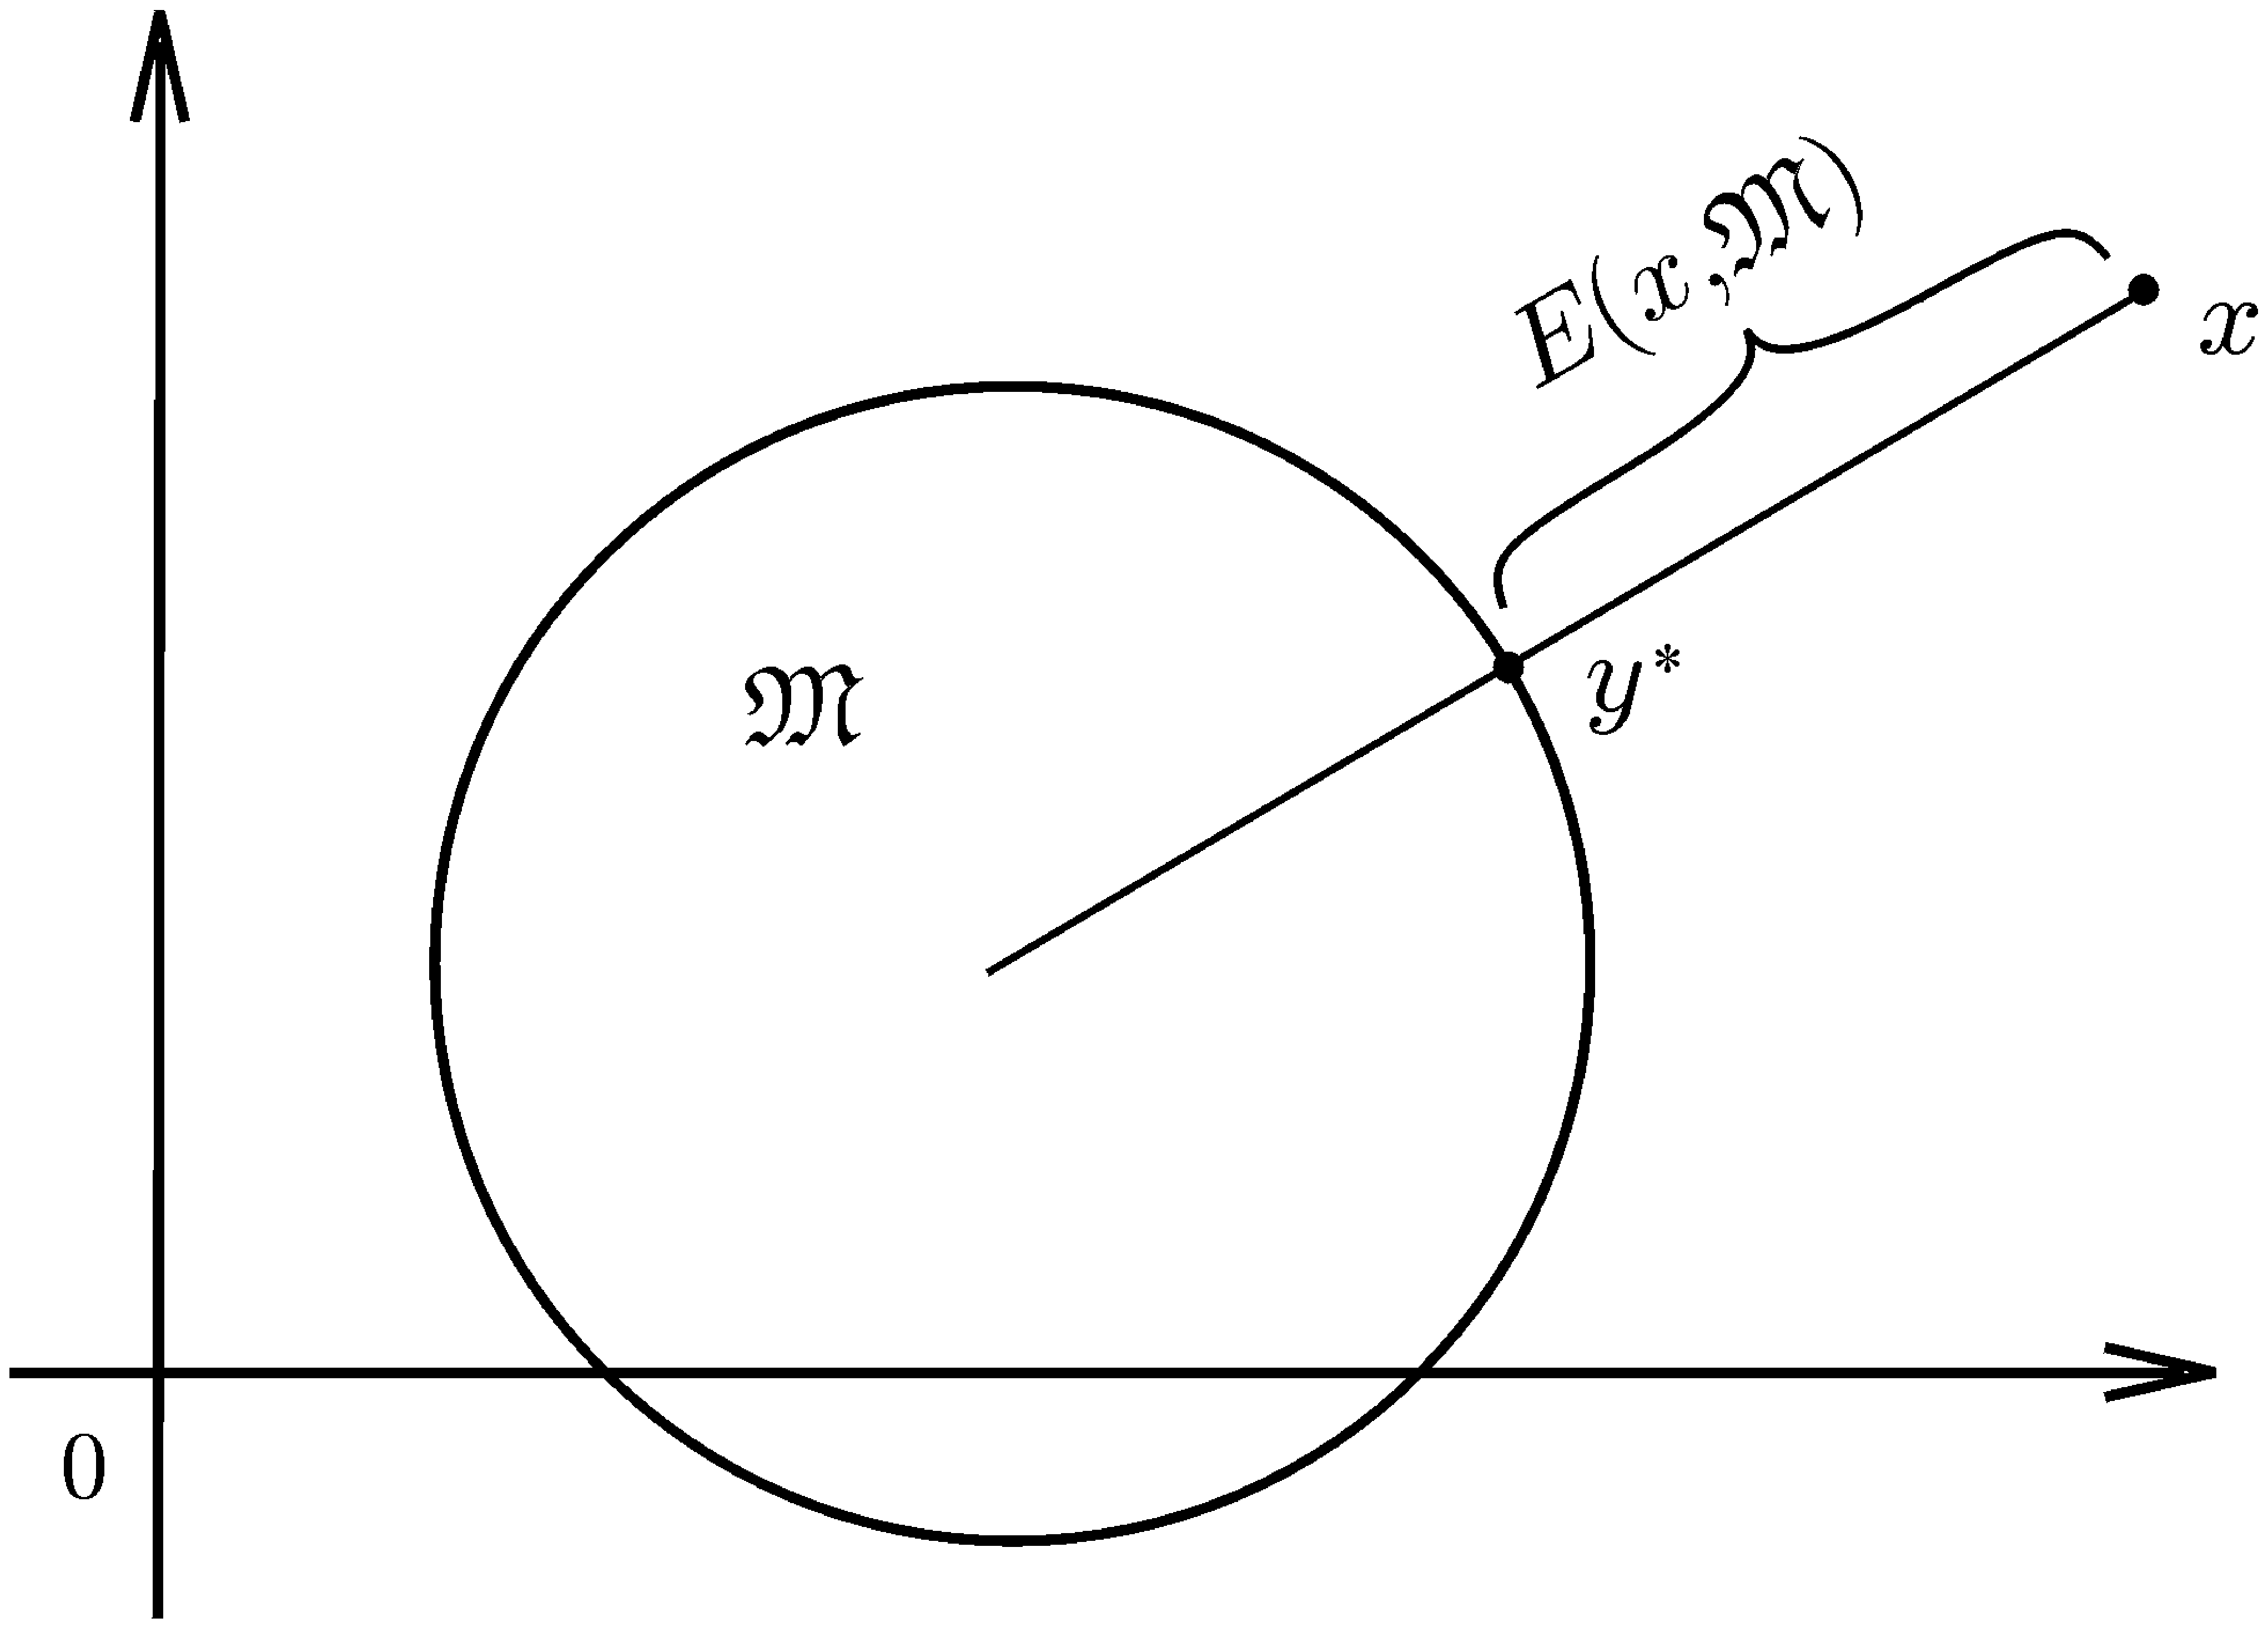
\includegraphics[width=0.5\textwidth]{pict/pict01-1.eps}
\end{center}
 \bigskip
 \refstepcounter{ris}\label{r1-1}

 \centerline{Рис.~\theris}
 \bigskip
\end{figure}

%%%%%%%%%%%%%%%%%%%%%%%%%%%%%%%%%%%%%%%%%%%%%%%%%%%%%%%%%%


Наилучшее приближение и наилучший элемент обладают и другими
неприятными особенностями. Поясним на
примере.

\begin{Example}
$X=C[a,b],$~ $-\infty < a < b < +\infty$ {(функция $f\in
C[a,b]$,} {если она непрерывна на $[a,b]$)},
{$\|f\|_C=\max\limits_{x\in[a,b]}|f(x)|$,}
$\ro(f,g)=\|f-g\|_C$. В качестве $\G M$ возьмем $\G M=\{c \}$
{--} множество констант $c \in \bR${, точнее, множество}
{постоянных функций}. Тогда, очевидно, {для любой} $ f
\in C[a,b]$ существует единственный наилучший элемент $c^* \in
\G M$, {
$$
c^* = \frac{\max\limits_{x\in[a,b]}{f(x)}+\min\limits_{x\in[a,b]} {f(x)}}{2}
$$
}
(см. рис.~\ref{r1-2}).
\end{Example}

%%%%%%%%%%%%%%%%%%%%%%%%%%%%%%%%%%%%%%%%%%%%%%%%%%%%%%
%\vspace{5mm}

\begin{figure}[ht]
\begin{center}
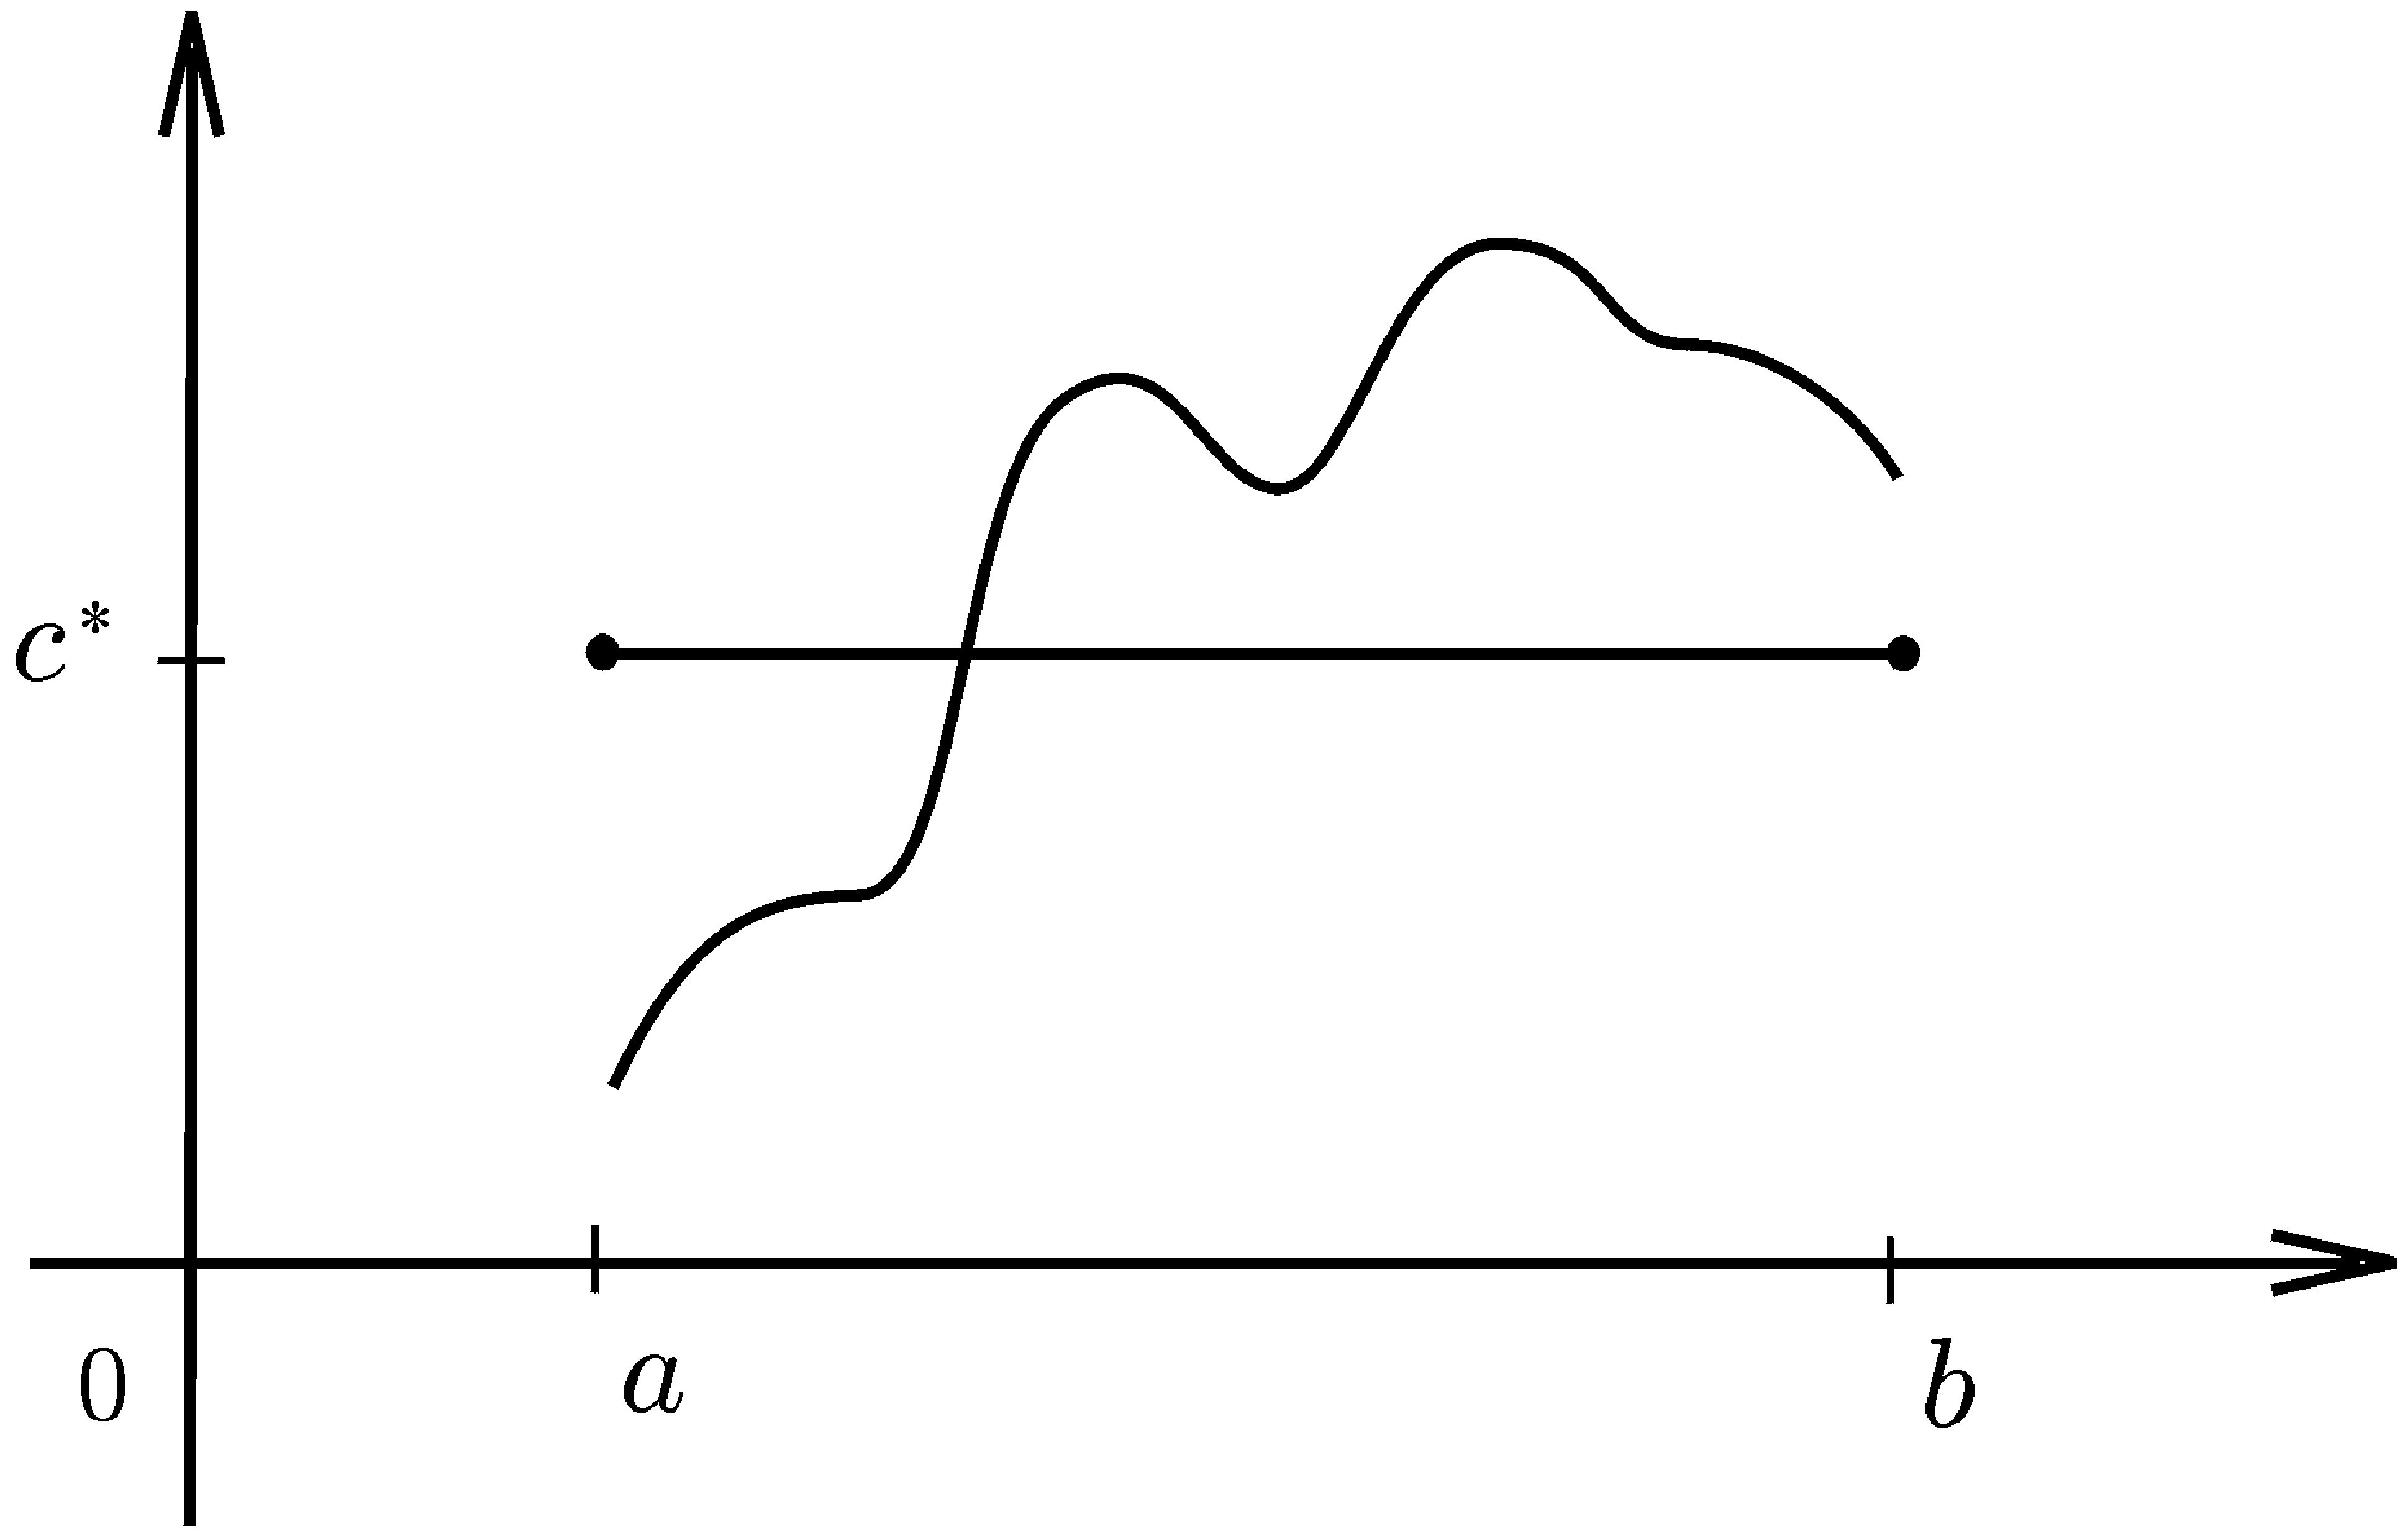
\includegraphics[width=0.5\textwidth]{pict/pict01-2.eps}
\end{center}
 \bigskip
 \refstepcounter{ris}\label{r1-2}

 \centerline{Рис.~\theris}
 \bigskip
\end{figure}

% \bigskip
% \begin{picture}(70,170)
% \put(100,160){\special{em: graph pict01-2.eps}}
% \end{picture}
% \refstepcounter{ris}\label{r1-2}

% \centerline{Рис.~\theris}
% \bigskip

%%%%%%%%%%%%%%%%%%%%%%%%%%%%%%%%%%%%%%%%%%%%%%%%%%%%%%%%%%



Итак, возникает оператор {наилучшего приближения} $A${,}
любой функции $f \in C[a,b]$ ставящий в соответствие
наилучший элемент $c^* \in \G M$: $A(f)=c^*(f).$ Этот оператор не является линейным.
Действительно, если мы возьмем $f_1$ и $f_2$ как на рис.~\ref{r1-3}, то
$c^*(f_1)=c^*(f_2)=c^*(f_1+f_2)=h/2,$ т.\,е. $A(f_1+f_2)\ne A(f_1)+A(f_2).$

%%%%%%%%%%%%%%%%%%%%%%%%%%%%%%%%%%%%%%%%%%%%%%%%%%%%%%
%\vspace{5mm}

\begin{figure}[ht]
\begin{center}
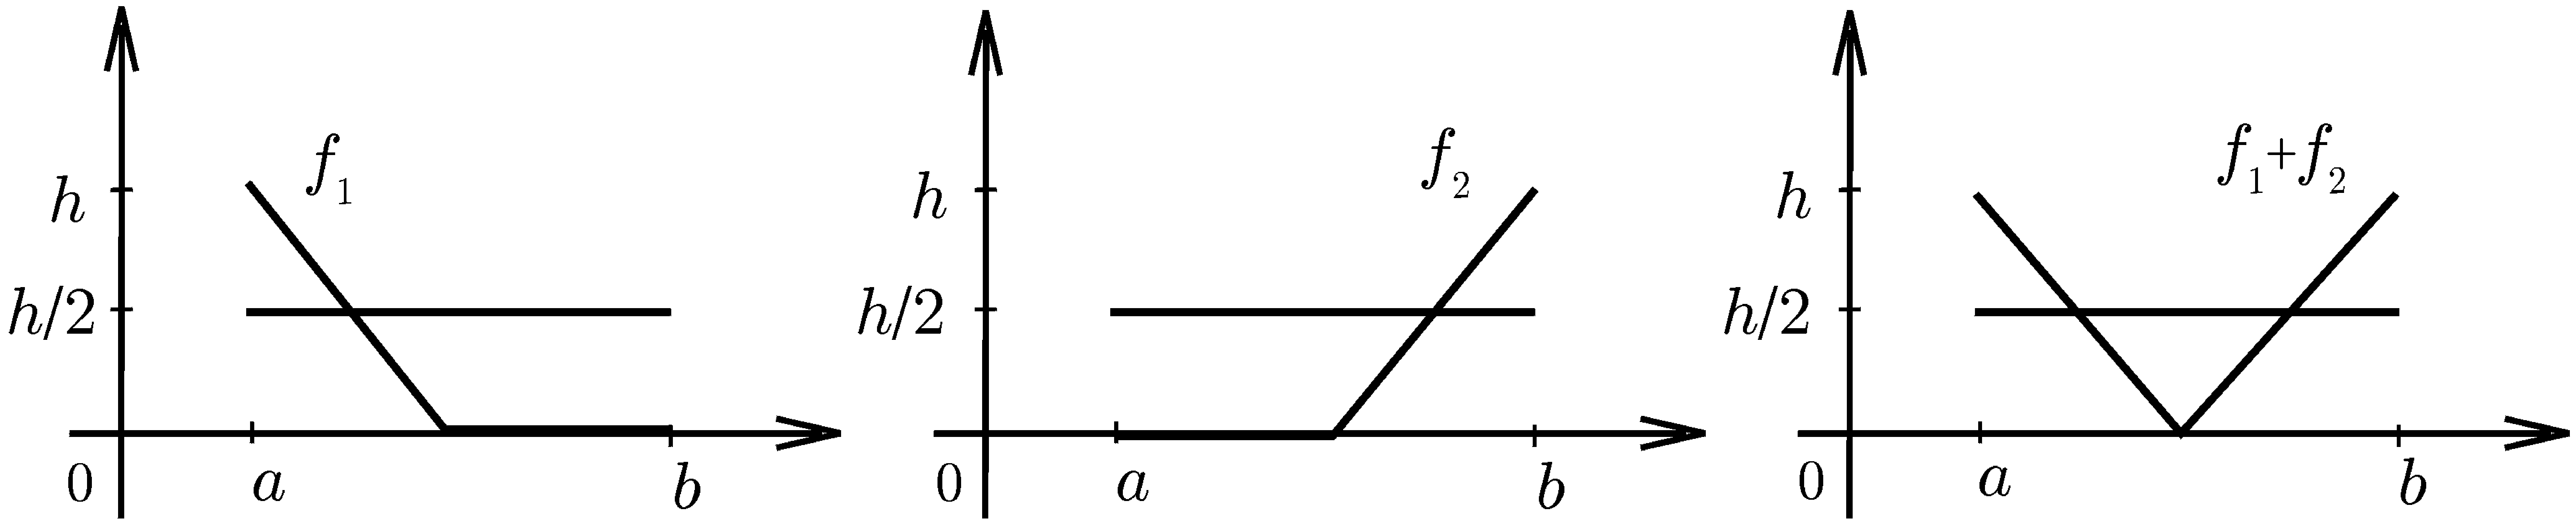
\includegraphics[width=0.9\textwidth]{pict/pict01-3.eps}
\end{center}
 \bigskip
 \refstepcounter{ris}\label{r1-3}

 \centerline{Рис.~\theris}
 \bigskip
\end{figure}



% \bigskip
% \begin{picture}(0,120)
% \put(-10,120){\special{em: graph pict01-3.pcx}}
% \end{picture}
%\centerline{рис. 3} \vspace{5mm}
% \refstepcounter{ris}\label{r1-3}

% \centerline{Рис.~\theris}
% \bigskip

Итак, в некоторых функциональных пространствах {оператор наилучшего} {приближения}
$A$ не является линейным, значит,
{найти} $E{(x)}$ и $y^*{(x)}$ {может} {оказаться трудной задачей. Поэтому рассматривают и
более простые методы} {приближения. В частности, различные линейные методы.}

\section{Линейная задача теории приближения}

Пусть $X=C[a,b]=C$ и $\Cal L$ -- некоторое {подпространство} из $C$ и пусть $A$~--
линейный оператор из $C$ в $C$ и {$Af \in \Cal L$} для любой функции $f \in C[a,b].$
Будем говорить в этом случае, что в $C$ задан линейный метод $A$ приближения элементов
{из} $C$ посредством подпространства $\Cal L$. {Для $f$ в качестве приближающего
выступает элемент $Af$.}

Интерполирование -- первый классический метод линейного приближения.

\section{Лагранжево интерполирование}

Пусть функция $f \in C[a,b]$ (пока можно считать, что значения $f(x) \in \bC$~--
множеству комплексных чисел).

Возьмем на $[a,b]$ {различные точки} $x_k\ (k=0,1,\ldots,n)$. Можно считать, что
$a \le x_0 <x_1< \cdots <x_n \le b.$ Точки $\{x_k\}$ будут называться {\it узлами
интерполяции}.

Задача состоит в том, чтобы для узлов $\{x_k\}$ и для любого набора {чисел} $\{y_k\}\
(k=0,1,\dots ,n)$ построить многочлен $p_n \in \mathcal{P}_n,$
\[
  p_n(x)=a_0+a_1x+\cdots +a_n x^n,
\]
такой, что $p_n(x_k)=y_k$\  $(k=0,1,\dots ,n).$

Возникают вопросы:
\smallskip
1) Всегда ли задача разрешима?
\smallskip
2) Сколько имеется решений?
\smallskip

Здесь для определения коэффициентов $a_i\ (i=0,1,\dots,n)$ получается система линейных
уравнений с определителем Вандермонда, не равным $0.$ Следовательно, для любых $x_k$ и
любых $y_k$ имеется единственное решение. Поэтому достаточно {выписать} решение в
явном виде. {С этой целью для} любого $k=0,1,\dots,n$ построим фундаментальный
многочлен {$l_k(x)$} лагранжевой интерполяции, соответствующий $k$-му узлу, -- это
многочлен степени $n$, обладающий свойствами: $l_k(x_i)=\delta_{i,k}$, где
$\delta_{i,k}$ -- символ Кронекера, $\delta_{k,k}=1, \ \delta_{i,k}=0$ при $i \ne k$.

Очевидно,
\[
  l_k(x)=\frac{(x-x_0)(x-x_1)\cdots (x-x_{k-1})(x-x_{k+1})\cdots (x-x_n)}
         {(x_k-x_0)(x_k-x_1)\cdots (x_k-x_{k-1})(x_k-x_{k+1})\cdots (x_k-x_n)}.
\]
Обозначим $\omega(x)=\prod_{k=0}^n(x-x_k).$
Тогда
$$
\omega'(x_k)=
      (x_k-x_0)(x_k-x_1)\cdots (x_k-x_{k-1})(x_k-x_{k+1})\cdots (x_k-x_n)
$$
и, следовательно,
\[
 l_k(x)=\frac{\omega(x)}{(x-x_k)\omega'(x_k)}.
\]
Ясно, что
\[
 p_n(x)=p_{n}(x,\{y_k\},\{x_k\})=
 %\sum_{k=0}^n y_k
 %\frac{\omega(x)}{(x-x_k)\omega'(x_k)}=
 \sum\limits_{k=0}^n y_k l_k(x)
\]
-- искомый многочлен. Интерполяционный многочлен
рассматриваемой задачи, записанный в этой форме, называется {\it
интерполяционным многочленом Лагранжа}.

Пусть теперь $f \in C[a,b],$~ $\{x_k\}$~-- узлы интерполяции, а $y_k=f(x_k)$\
$(k=0,1,\dots ,n).$ Тогда для любой функции $f \in C[a,b]$ и любых узлов
{интерполяции} $\{x_k\}$\  $(k=0,1,\dots ,n)$ существует единственный многочлен
$$
p_n(x,f)=p_n(x,f,\{x_k\})=\sum\limits_{k=0}^n f(x_k) l_k(x)
$$
степени не выше $n$, который удовлетворяет условиям
\[
 p_n(x_k,f)=f(x_k)\qquad (k=0,1,\dots ,n).
\]
Таким образом, возникает {оператор} $P_n:\ f \longmapsto p_n(x,f)$ {из} $C{[a,
b]}$ в $C{[a,b]}$. {Отметим} простейшие свойства {этого оператора.}

1) {Если} $f \in \Cal P_n$, то для любых узлов $\{x_k\}$
имеем $p_n(x,f)\equiv f(x),$ т.\,е. $P_{n}(f)=f.$

2) $f \to P_n(\cdot,f)$
~-- линейный (т.\,е. однородный, аддитивный) ограниченный оператор:
$$
  P_n(c_1f_1+c_2f_2) \equiv c_1P_n(f_1)+c_2P_n(f_2),\qquad
  f_i\in C[a,b],\qquad c_i\in \bR\qquad (i=1,2),
$$
и для любой функции
$f\in C[a,b]$
$$
  \|p_n(\cdot,f)\|_C \le L_n\|f\|_C,\ \ \mbox{где}\ \
  L_n=\|P_n\|_C^C<\infty.
$$

Более того,
$$
|p_n(x,f)| \le L_n(x)\|f\|_C.
$$
Здесь $L_n(x)=\sum{|l_k(x)|},$~ $L_n =
\|L_n(x)\|_C$. Оба неравенства вытекают из формулы для $p_n(x, f) = p_n(x,f,\{x_k\})$. В
пространстве $C[a,b]$ они являются точными.

{Действительно, определим
при фиксированном $\xi \in [a,b]$ функцию $f_\xi(x)$ так,
чтобы она удовлетворяла условиям}

{а) $f_\xi(x)=\sign{l_k(\xi)}$ при $x=x_k\  ( k=0,1,\ldots,n)$,}

{б) $|f_\xi(x)| \le 1$ при $x \in [a,b]$,}

{в) $f_\xi(x)$ непрерывна по $x$ на $[a,b]$.}

{Тогда будем иметь
$$
\|f_\xi\|_C=1,
\qquad  p_n(x, f_\xi) = \sum\limits^n_{k=0}{f_\xi(x_k)l_k(x)}
$$
и, в частности,
$$
  p_n(\xi, f_\xi) = \sum\limits^n_{k=0}{|l_k(\xi)|} =
  L_n(\xi)\|f_\xi\|_C,
$$
а выбирая здесь в качестве $\xi$ точку $x^*$ максимума на $[a,b]$ функции $L_n(x)$,
получим
$$
  p_n(x^*,f_{x^*}(\cdot)) = L_n\|f_{x^*}\|_C
$$
и, следовательно,
$$
  \|p_n(x,f_{x^*}(\cdot))\|_C = L_n\|f_{x^*}\|_C.
$$}

{Таким образом, константа $L_n$ есть норма оператора $P_n\colon f \longmapsto p_n(x,f):$
$$
  \|P_n\|_{C \to C} = L_n.
$$
А для любого фиксированного $x \in [a,b]$ величина $L_n(x)$ является нормой функционала
$P_x(f)=p_n(x,f)$ в $C[a,b]$:
$$
\|P_x(f)\| = L_n(x),
$$
так как
$$
|P_x(f)| \le L_n(x)\|f\|_C\qquad \forall\ f \in C[a,b]
$$
и
$$
|P_x(f_x(\cdot))|=L_n(x)\|f_x\|_C.
$$}

{Константа $L_n$ называется \textit{константой Лебега}, а $L_n(x)$ --
\textit{функцией Лебега} линейного метода $p_n(x, f, \{x_k\})$ приближения функций $f$ из
$C[a,b]$ интерполяционными многочленами Лагранжа. Ясно, как эти понятия распространяются
на другие линейные методы приближения.}

{Метод интерполирования тем <<лучше>>, чем меньше его норма, т.\,е. константа Лебега. При
$n$ фиксированном $L_n$ зависит от узлов интерполирования $\{x_k\}$. Если $[a,b]=[-1,1]$,
то можно узлы выбрать так, что $L_n=\dfrac{2}{\pi}\ln{n} + O(1)$~ $(n \to +\infty)$, а
именно, в качестве узлов интерполяции нужно взять нули многочлена Чебышева
$$
T_{n+1}(x)=\cos({(n+1)}\arccos{x}).
$$}

3) Тождества Коши.

Из свойства 1) и формулы для интерполяционного многочлена {при $f(x)\equiv 1$}
получаем {тождество}
\[ \sum\limits_{k=0}^n l_k(x) \equiv 1, \]
{а при} $f(x)=(x-u)^j$~ $(j=1,\dots ,n;\ u\in \mathbb C)$ {-- тождества}
$$
(x-u)^j\equiv \sum\limits_{k=0}^n (x_k-u)^j l_k(x) \qquad (j=1,2,\ldots,n),
$$
{откуда при} $u=x$ следует, {что}
\begin{equation}\label{f1-1}
\sum\limits_{k=0}^n (x_k-x)^j l_k(x)\equiv 0\qquad (j=1,\ldots ,n).
\end{equation}
Эти тождества при $\{x_n\}\subset [a,b]$ справедливы для
всех $x\in \mathbb C.$

\section{Оценка погрешности интерполяционной \\ формулы
Лагранжа. Неравенства Лебега}

Пусть $\{x_k\}_{k=0}^n$~-- узлы интерполяции, $f \in C[a,b],$ $p_n(x,f)$ --
соответствующий интерполяционный многочлен Лагранжа. Можно написать
\[
  f(x)=p_n(x,f)+R_n(x,f),
\]
где $R_n(x,f)$~-- остаточный член. Очевидно, в узлах интерполяции $R_n(x_k,f)=0$~
$(k=0,\dots ,n).$ Требуется оценить $R_n(x,f)$ для любого фиксированного $x \in [a,b],$
а также оценить $\|R_n(\cdot ,f)\|_{C[a,b]}.$

Оказывается, для оценок остаточного члена лагранжевой интерполяции {достаточно} знать
$L_n(x),$ $L_n$ {и} $E(f ,\Cal P_n)_C=\inf\limits_{q \in \Cal P_n}\|f-q\|_{{C}}.$
Именно, имеют место неравенства Лебега
\[  |R_n(x,f)|\le (L_n(x)+1)E(f ,\Cal P_n)_C,             \]
\[  \|R_n(\cdot ,f)\|_{{C}} \le (L_n+1)E(f ,\Cal P_n)_C.             \]
Для доказательства воспользуемся тем, что $P_n(x,f)$~-- линейный оператор, и
$P_n(x,q)=q(x)$ для любого $q \in \Cal P_n$ ({аналогичные неравенства} Лебега
{возникают} и {для} более {общих линейных методов, сохраняющих элементы $\Cal
P_n$ на месте}). Имеем
\begin{multline*}
  |R_n(x,f)|=|f(x)-p_n(x,f)|=|f(x)-q(x)-p_n(x,f-q)|\le  \\
  \le |f(x)-q(x)|+L_n(x)\|f-q\| \le
      (L_n(x)+1)\|f-q\|_{{C}}, \qquad q \in \Cal P_n.
\end{multline*}
Значит, если в качестве $q$
возьмем наилучший элемент для $f$
в $\Cal P_n,$
то получим
\[  |R_n(x,f)|\le (L_n(x)+1)E(f ,\Cal P_n)_C,\qquad x\in [a,b],   \]
откуда следует, что
\[  \|R_n(\cdot ,f)\|_{{C}} \le (L_n+1)E(f ,\Cal P_n)_C.             \]

\section{Остаточный член в форме Коши\\
 для интерполяционной формулы Лагранжа}

%%%%%%%%%%%%%%%%%%%%%%%%%%%%%%%%%%%%%%%%%%%%%%%%%%%%%%%%%
{Функция $f \in C^{(n+1)}[a,b],$ если $f$ непрерывна на $[a,b]$ вместе с производными
до} {порядка $n+1$ включительно.}

\begin{teo}\label{t1-1}
Пусть $f \in C^{(n+1)}[a,b].$ Тогда для любого $x \in [a,b]$ существует {точка} $\xi
\in (a,b)$ {такая}, что
\[
  R_n(x,f)=\frac{f^{(n+1)}(\xi)}{(n+1)!}\omega (x)
\]
$(${здесь $\xi=\xi(x,f,\{x_k\})$},~ $n+1$~-- число узлов
интерполяции$).$
\end{teo}

\begin{proof}
{Доказываемая формула, очевидно, верна для $x=x_k$}
{$(k=0,\dots ,n)$} ($\xi$ может любой точкой). Зафиксируем {$x \in [a,b],$~ $x \ne x_k,$}
и рассмотрим вспомогательную функцию
\[
  F(t)=f(t)-p_n(t)-K\omega (t),
\]
где {$p_n(t)=p_n(t,f,\{x_k\}),$~ $K=R_n(x,f)/ \omega (x), \ \omega(x) \ne 0.$} Заметим,
что $F(t)$ при $t=x_k$ равна нулю $(k=0,\dots ,n)$ и $F(x)=0$ по выбору $K.$ Следовательно, функция
{$F(t)$} имеет нули в ${n+2}$ различных точках. Применим обобщенную теорему Ролля, из
которой следует, что найдется точка $\xi \in (a,b)$ такая, что $F^{(n+1)}(\xi)=0$.
{Но} $F^{(n+1)}(\xi)=f^{(n+1)}(\xi)-K\cdot (n+1)!,$ значит,
$K=f^{(n+1)}(\xi)/(n+1)!,$ откуда {для} $R_n(x,f)=K\omega(x)$ {получаем}
\[
  R_n(x,f)=\frac{f^{(n+1)}(\xi)}{(n+1)!}\omega (x)
\]
и теорема доказана.
\end{proof}

\begin{Remark}[геометрическое]
{Остаточный} член не обязан менять знак в узлах {интерполяции вслед за
$\omega(x).$} Графики $f(x)$ и $p_n(x,f)$ могут соприкасаться, как показано на
рис.~\ref{r1-4}.
\end{Remark}

%%%%%%%%%%%%%%%%%%%%%%%%%%%%%%%%%%%%%%%%%%%%%%%%%%%%%%
%\vspace{5mm}

\begin{figure}[ht]
\begin{center}
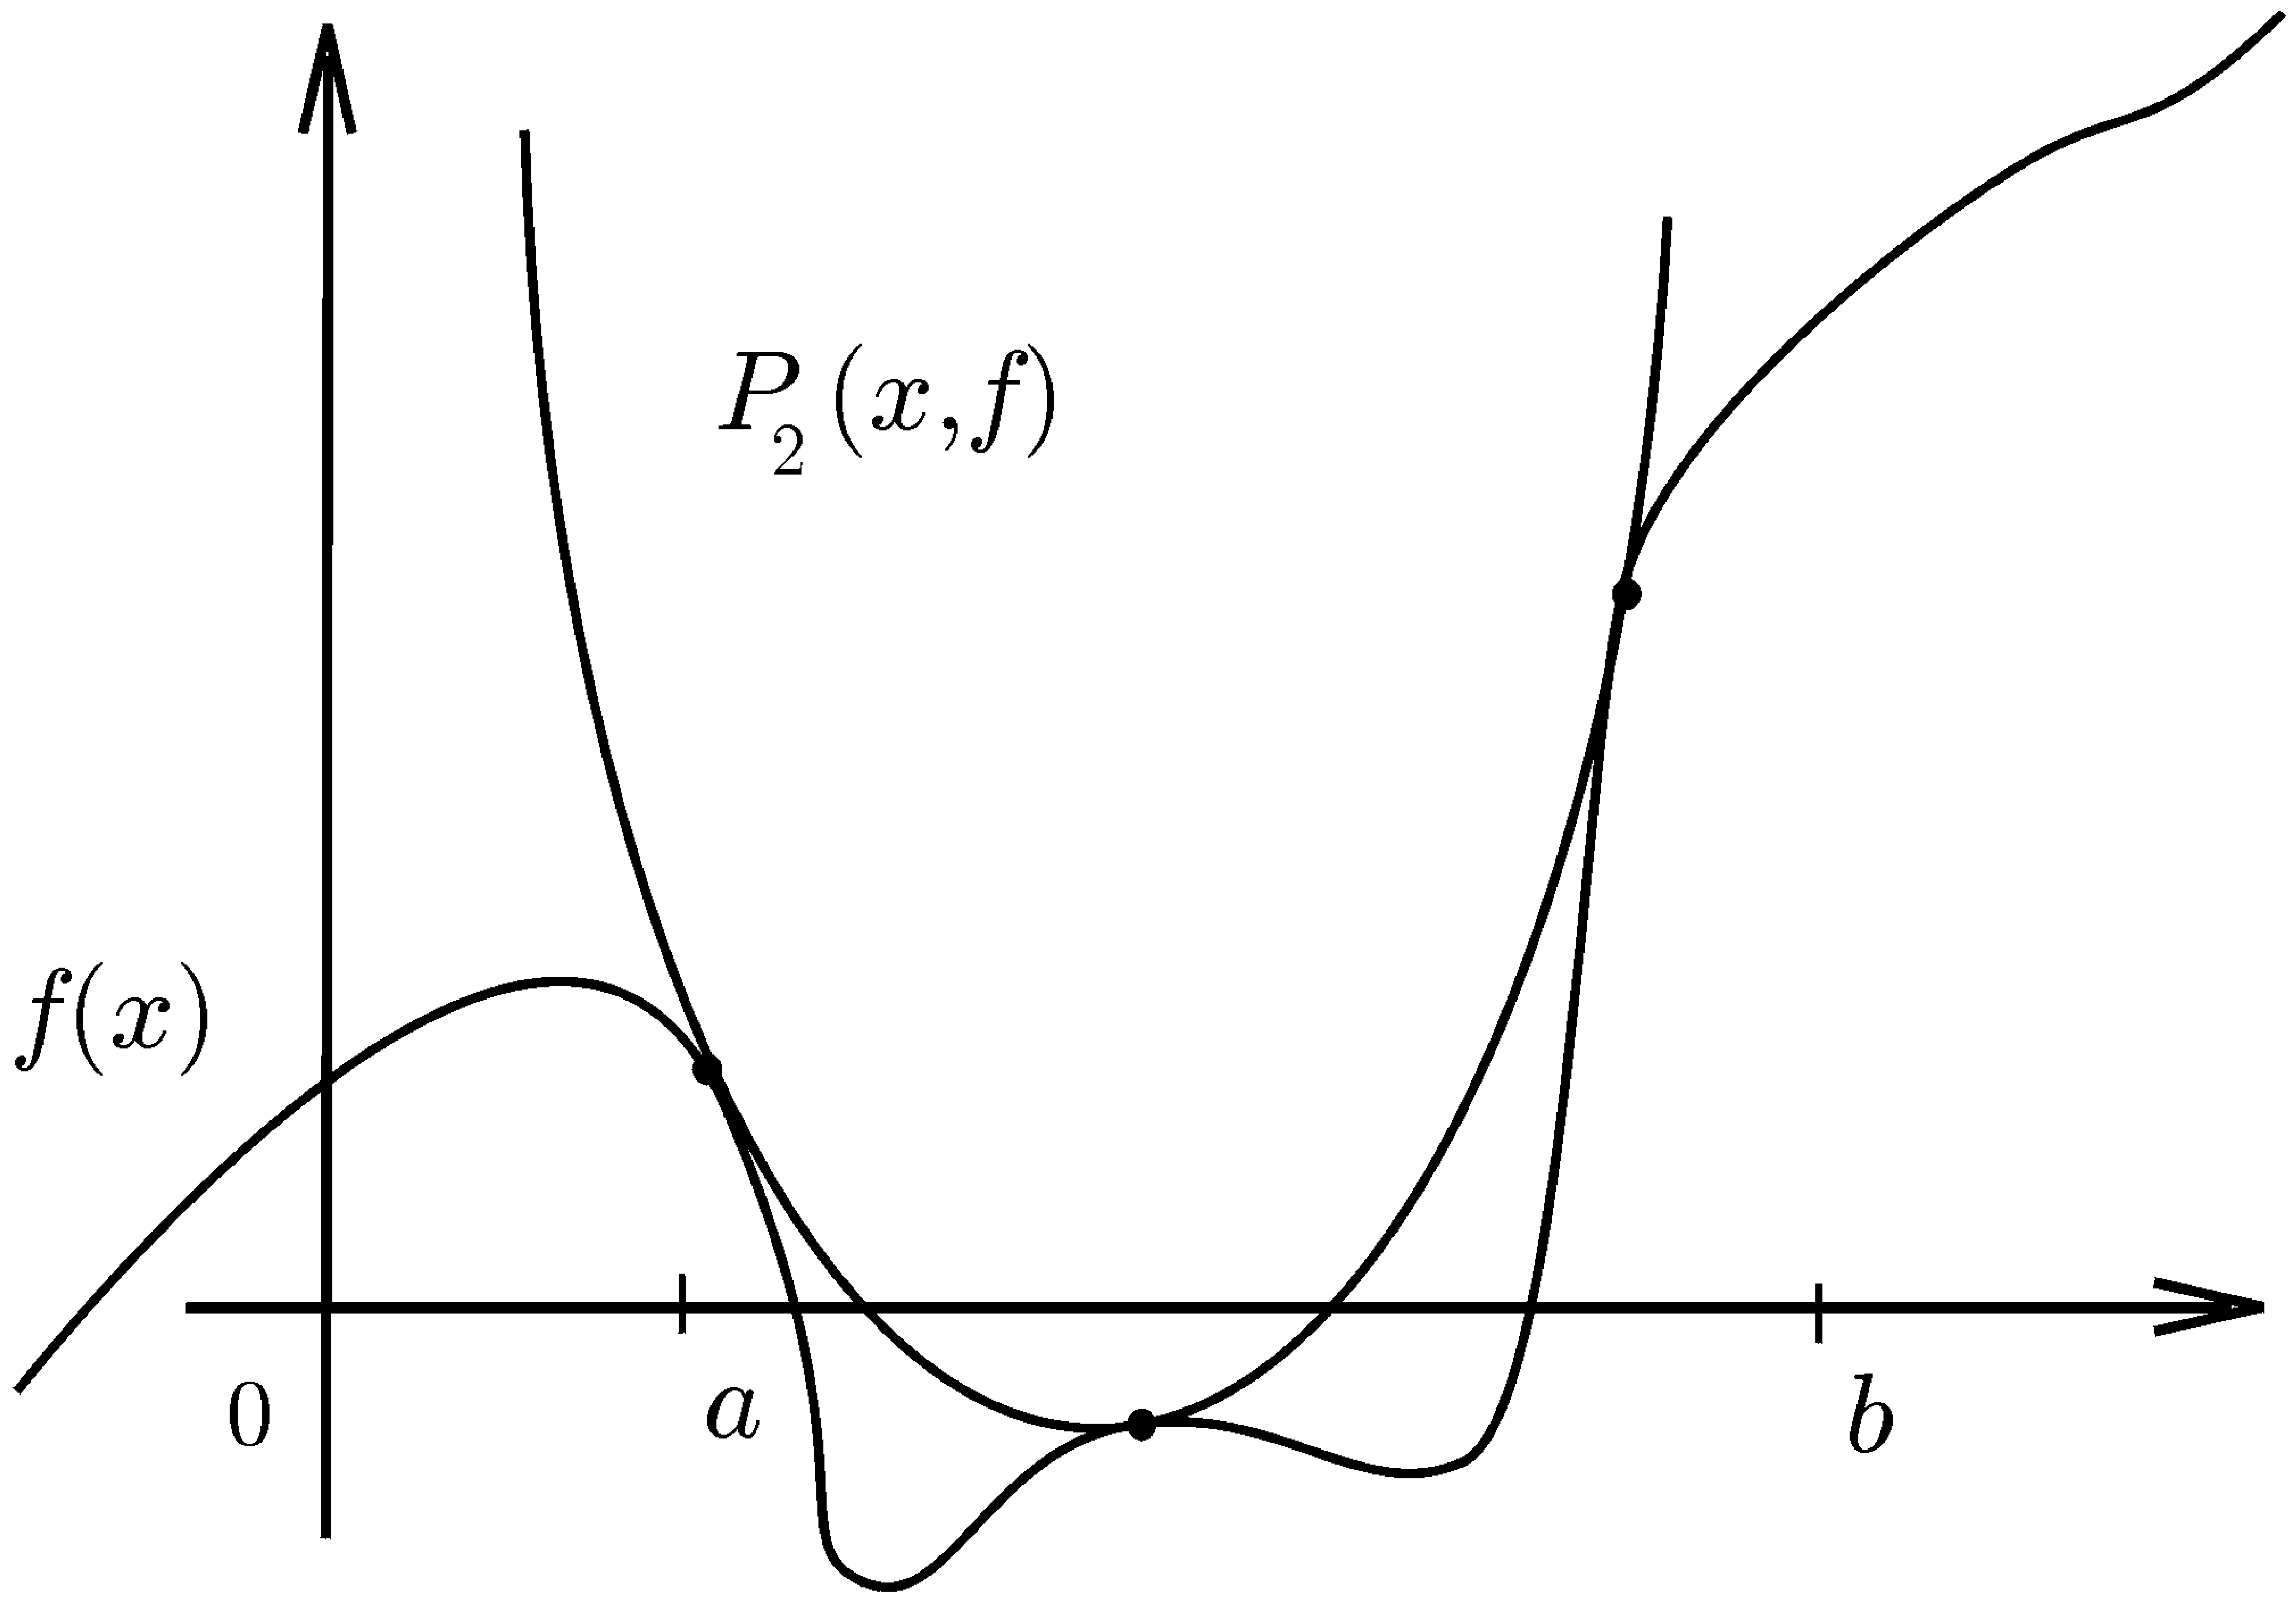
\includegraphics[width=0.5\textwidth]{pict/pict01-4.eps}
\end{center}
 \bigskip
 \refstepcounter{ris}\label{r1-4}

 \centerline{Рис.~\theris}
 \bigskip
\end{figure}



% \bigskip
% \begin{picture}(70,190)
% \put(90,190){\special{em: graph pict01-4.pcx}}
% \end{picture}
%\hbox to 0.5cm {}{\special{em:graph pict4.pcx}}
%\vspace{6cm}

% \refstepcounter{ris}\label{r1-4}

% \centerline{Рис.~\theris}
% \bigskip

%%%%%%%%%%%%%%%%%%%%%%%%%%%%%%%%%%%%%%%%%%%%%%%%%%%%%%%%%%
%\noindent \hskip3.0cm {\rm рис. 4}
%\bigskip



Но есть достаточное условие того, что остаточный член меняет знак в узлах. Как видно из
формулы для остаточного члена интерполяции в форме Коши, {\it если} $f^{(n+1)}(x)$
{\it сохраняет знак}, {\it то} $R_n(x,f)$ {\it меняет знак в узлах интерполяции и только в них}.

Обозначим $M_{n+1}(f)=\max\limits_{x \in [a,b]}f^{(n+1)}(x).$

\begin{Corollary}
\[
 \|R_n(\cdot ,f) \|_C \le \frac{M_{n+1}(f)}{(n+1)!}\|\omega(\cdot ) \|_C .
\]
\end{Corollary}

\begin{task}
При каком выборе узлов интерполяции величина $\|\omega(\cdot ) \|_C$
наименьшая?
\end{task}

 Оказывается {это будет,} когда $\omega$~-- многочлен
Чебышева\footnote{{Свойства} многочлена Чебышева приводятся в лекции 2.}
{$\widetilde{T}_{n+1}(x,I)$ $(I=[a,b]).$}
{Действительно, } $\omega(x)=x^{n+1} +a_{n}x^n+ \dots +a_0.$ Так {что}
\[
  \inf \|\omega(\cdot)\|_{C[a,b]}=\|\widetilde{T}_{n+1}(\cdot{, I})\|_{C[a,b]},
\]
где $\widetilde{T}_{n+1}{(\cdot, I)}$~-- многочлен Чебышева
на $[a,b],$ т.\,е. наименее
уклоняющийся на $[a,b]$ от нуля многочлен {степени $n+1$} со
старшим коэффициентом 1. В частности, $\widetilde{T}_{n+1}(x,[-1,1])=
\dfrac1{2^n}\cos(n+1)\arccos x.$


\section{Теорема Хаара об интерполяции в $\mathbb R^N$}

Мы рассматривали {задачу} интерполяции на {$D=[a,b] \subset
\bR^1$} т.\,е. в одномерном случае. Пусть теперь множество {$D \subset \bR^N,\ N\ge 2.$}

{{В о п р о с ы}. \hspace{1em}}

Имеет ли смысл задача {интерполяции} в многомерном случае?

Существуют ли действительные функции {$f_0(x),f_1(x),\dots,f_n(x),$~ $x \in
\overline{D} \subset \bR^N,$} ({\it интерполяционные системы на} $D$), {линейными
комбинациями которых} можно интерполировать {любой набор чисел $\{y_k\}_{k=0}^n$ в} любых
{несовпадающих узлах} $\{x_k\}_{k=0}^n \in D?$

Легко убедиться, что интерполяционные системы, состоящие из
разрывных функций, существуют на любом множестве мощности континуум. Для
этого достаточно рассмотреть взаимно однозначное
отображение отрезка на множество и взять порожденные им функции,
соответствующие рассмотренной нами на отрезке
интерполяционной системе $1,x,x^2,\dots ,x^n.$

Далее будет показано, что задача интерполяции многочленами разрешима
в комплексной области. А ответ на вопрос об $\bR^N$ дает следующая теорема.

\begin{teo}[А.\,Хаар]
Если $N>1$ и множество $D\subset \mathbb R^N$ имеет
внутренние точки, т.\,е. {$\inter {D} \ne \varnothing,$} и если $n \ne 0,$ то {в
$D$ не существует} непрерывных действительных интерполяционных систем {$($т.\,е.
систем, которыми можно интерполировать} при любом выборе узлов $\{x_k\}^{n}_{k=0}$
любой набор чисел $\{ y_k\}_{k=0}^n).$
\end{teo}

\begin{proof}
Возьмем внутреннюю точку и ее некоторую
окрестность $\Delta \subset D,$
и пусть {$\{x_k\}_{k=0}^n \subset \Delta.$}

%%%%%%%%%%%%%%%%%%%%%%%%%%%%%%%%%%%%%%%%%%%%%%%%%%%%%%

\begin{figure}[ht]
\begin{center}
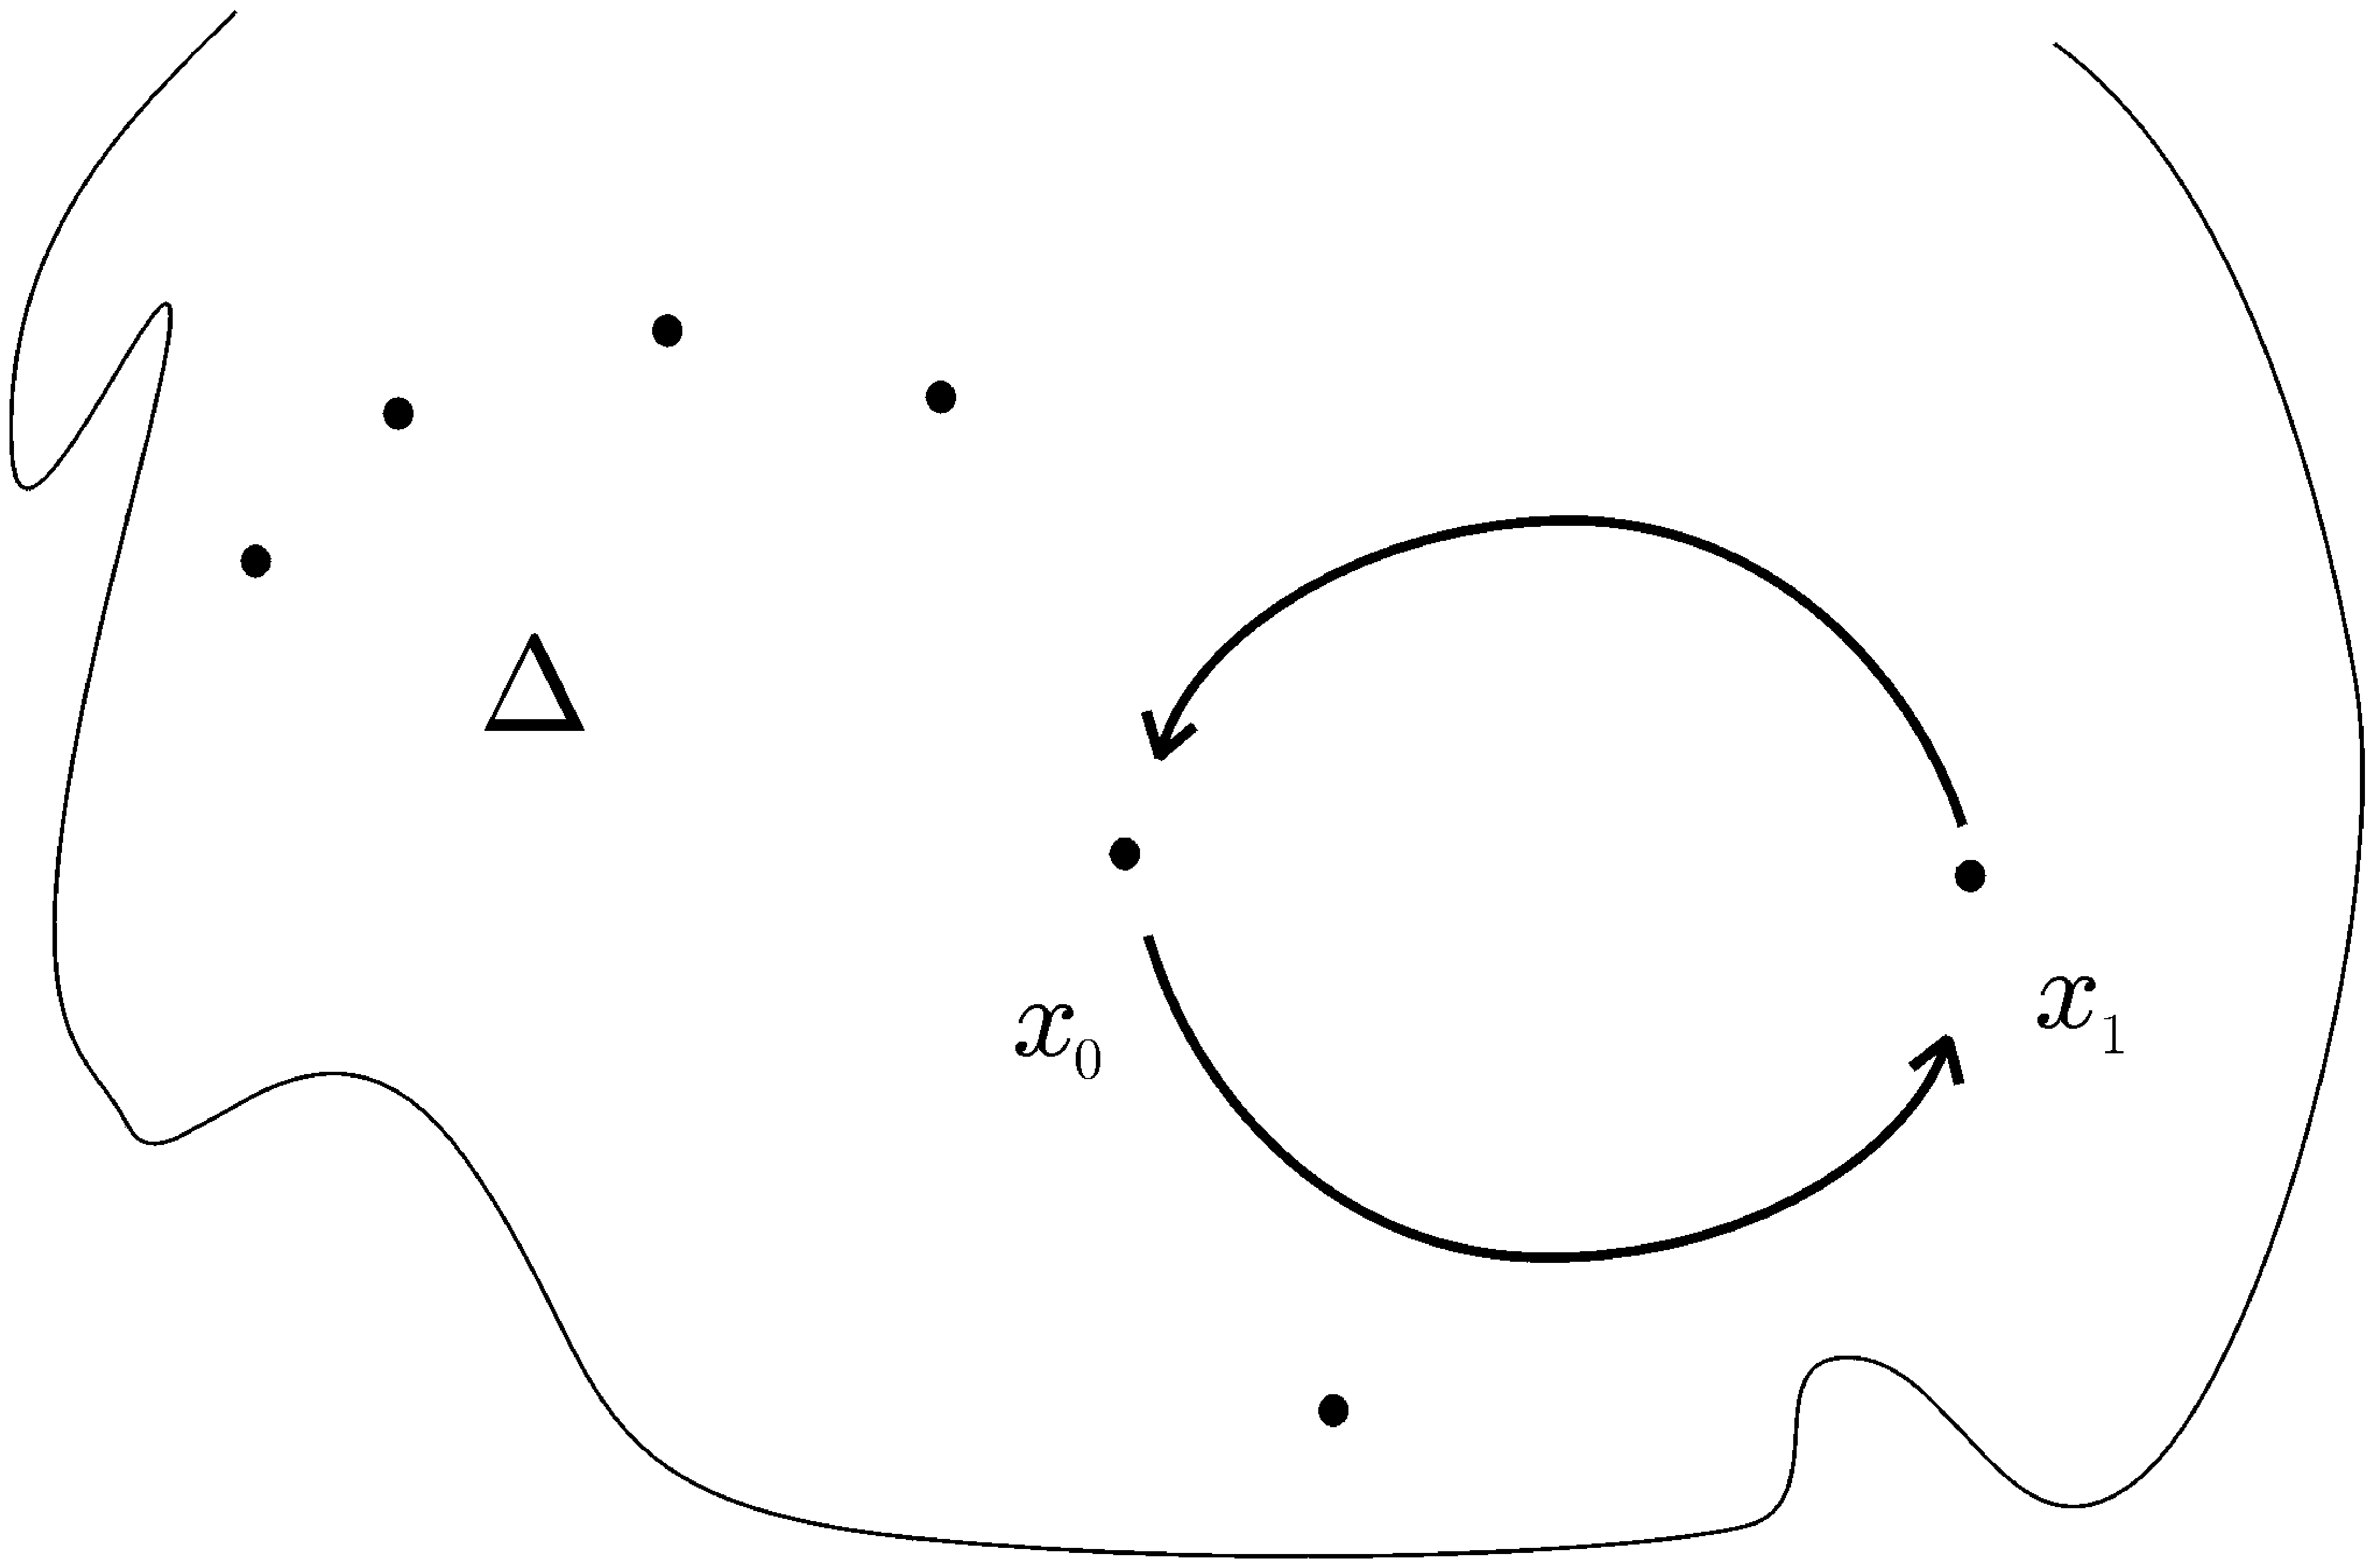
\includegraphics[width=0.5\textwidth]{pict/pict01-5.eps}
\end{center}
 \bigskip
 \refstepcounter{ris}\label{r1-5}

 \centerline{Рис.~\theris}
 \bigskip
\end{figure}




\noindent Если система {$\{f_k\}$~ $(k=0,\ldots,n)$} интерполяционная, то система
уравнений
\[
  \sum\limits^{n}_{k=0}c_k f_k(x_i)=y_i\qquad ({i}=0,\dots ,n),
\]
разрешима для любых {наборов чисел $\{y_k\}$}. {Отсюда следует, что} $\det
(f_k(x_i)) \ne 0$ {для любых $\{x_k\} \subset \Delta$.} По условию функции
$f_k$ непрерывны, следовательно, определитель непрерывен как функция от точек
$\{x_i\}$ в области $\Delta.$ Теперь все точки $x_k$ в $\Delta,$ кроме двух, например
$x_0$ и $x_1$, оставим на месте, а $x_0$ и $x_1$ будем непрерывно переводить друг в
друга {(см. рис.~\ref{r1-5})} {так, что при движении все $n+1$ точки
остаются различными и принадлежат $\Delta$.} Определитель будет непрерывно меняться,
{оставаясь вещественным,} и переменит знак (поменяются местами две строки
определителя). Следовательно, { при каком-то} {промежуточном наборе точек он
обращался в нуль. Это противоречие доказывает } {теорему. }
\end{proof}

\begin{Remark}
Непрерывные действительные интерполяционные
системы не существуют не только на множествах с непустой
внутренностью, но даже на континууме
с точкой ветвления.
\end{Remark}
Действительно, поменяем точки $x_0$ и $x_1$ {местами, перемещая их непрерывно,} как
показано на рис.~\ref{r1-6}, знак определителя изменится, следовательно, он обращался в
нуль, чего  не {должно} быть для непрерывных интерполяционных систем.

%%%%%%%%%%%%%%%%%%%%%%%%%%%%%%%%%%%%%%%%%%%%%%%%%%%%%%
 \bigskip
\begin{figure}[h]
\begin{center}
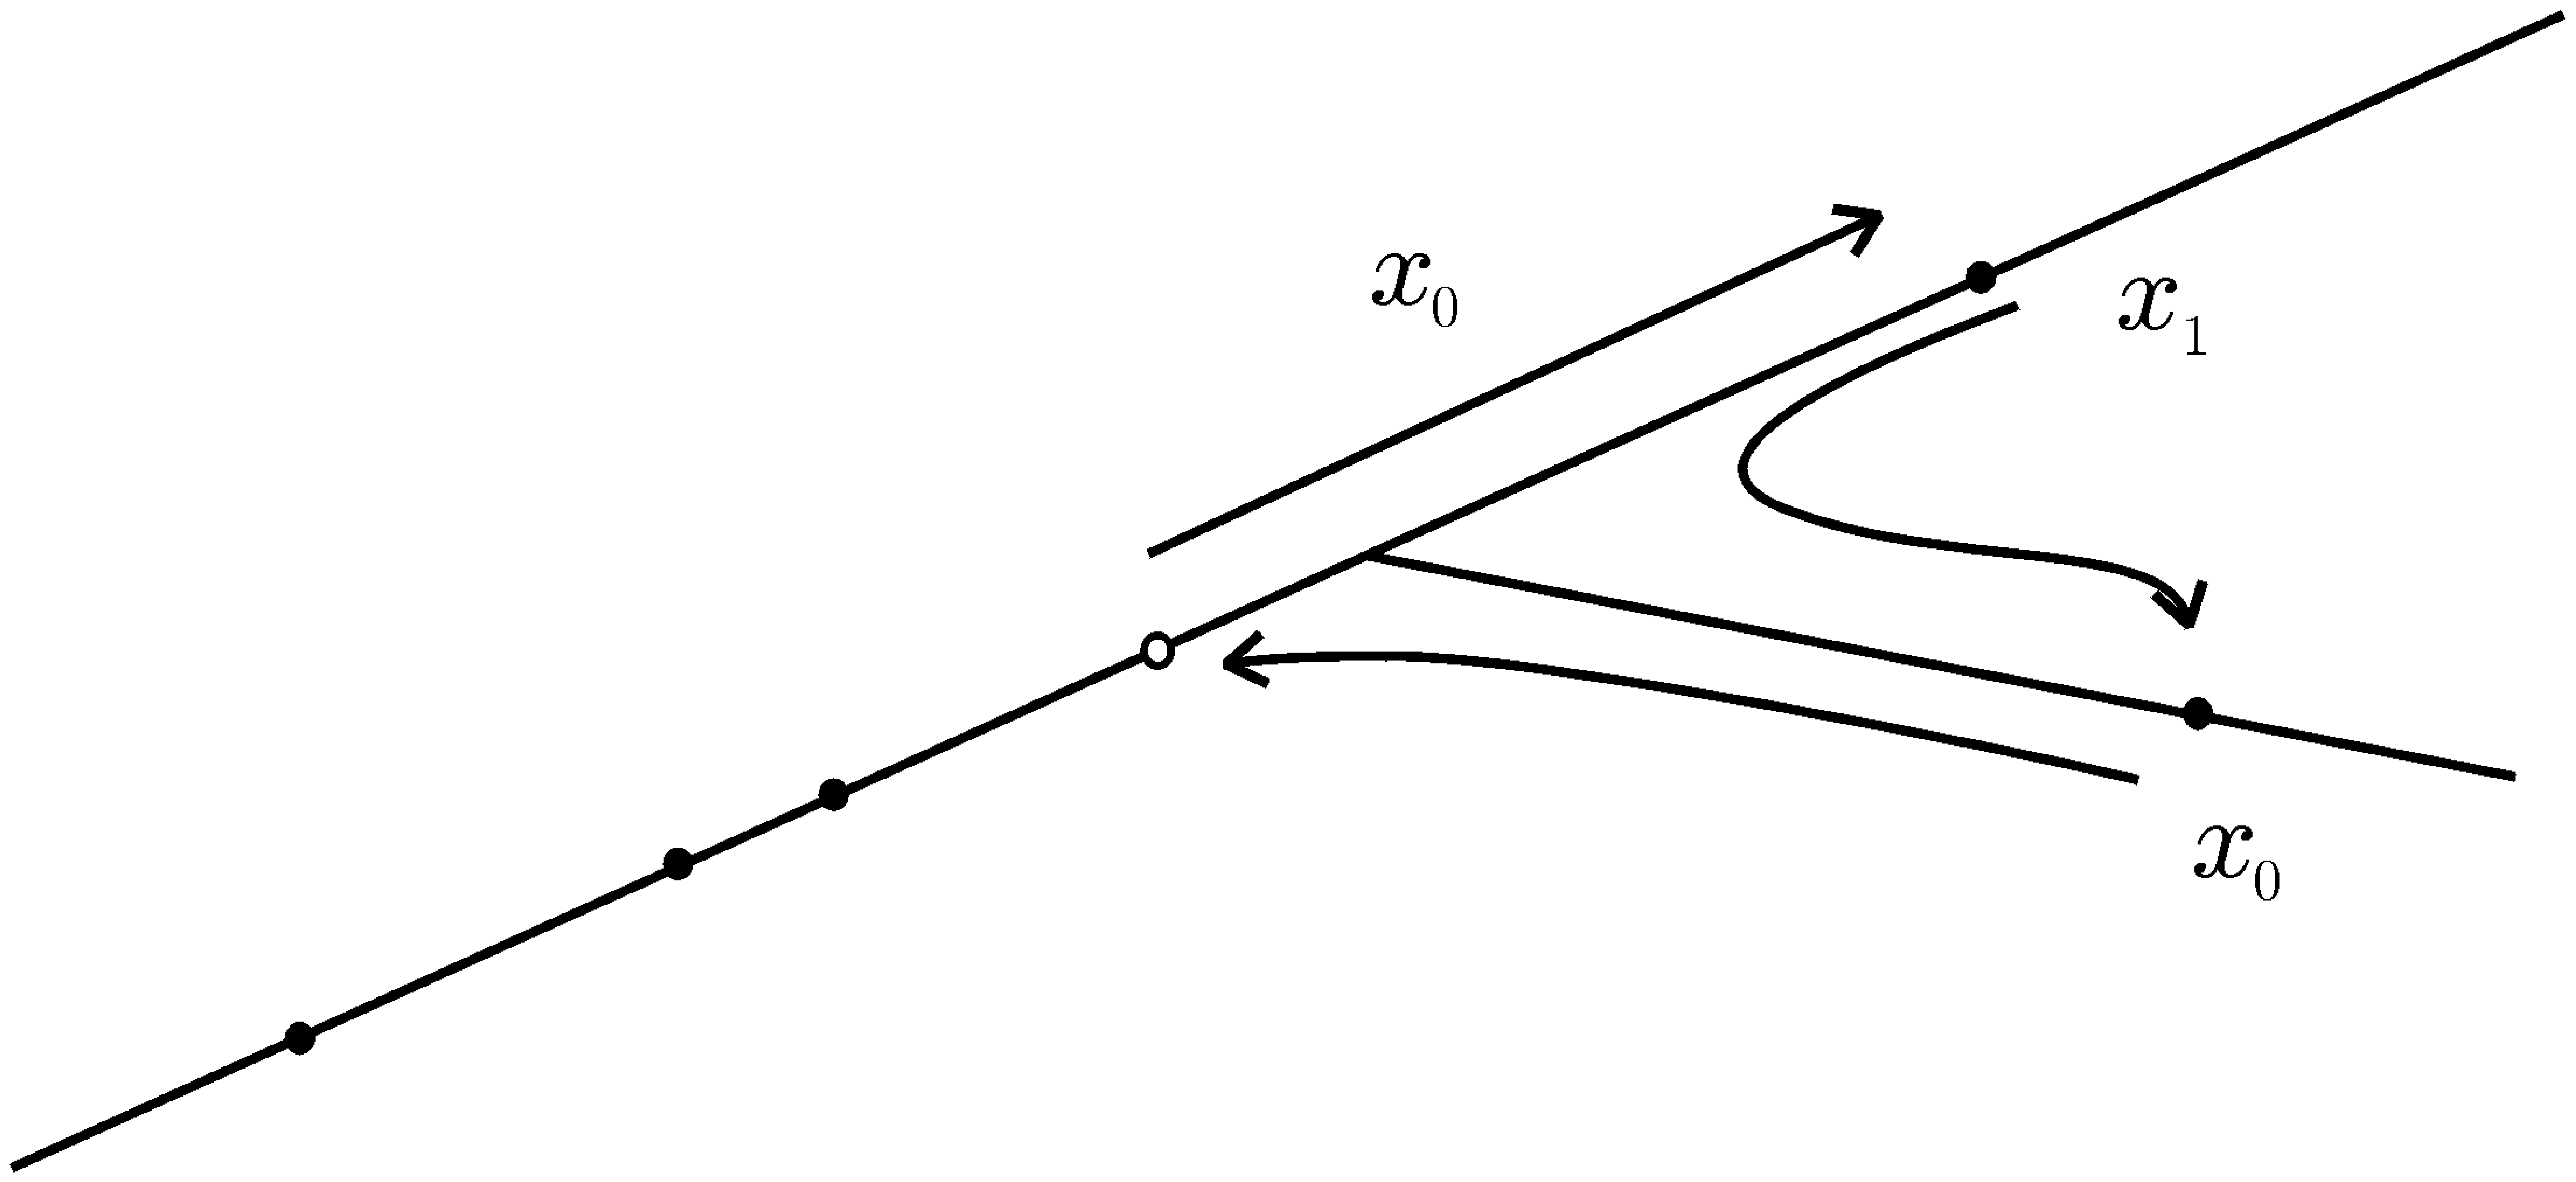
\includegraphics[width=0.5\textwidth]{pict/pict01-6.eps}
\end{center}
 \bigskip
 \refstepcounter{ris}\label{r1-6}

 \centerline{Рис.~\theris}
 \bigskip
\end{figure}


%%%%%%%%%%%%%%%%%%%%%%%%%%%%%%%%%%%%%%%%%%%%%%%%%%%%%%%%%%
%\noindent \hskip3.0cm {рис. 6}
%\bigskip

\noindent
Так что классическая задача интерполяции ограничена
рассмотрением ее на отрезке.

\begin{task}
При чем здесь отрезок? Пусть {$f_k(x) \in \bR^m$}\  $\forall\ x \in K \subset
\bR^M$\ {$(k=0,1,\ldots,n).$} На каких множествах $K$ существуют
непрерывные интерполяционные системы, а для каких не существуют?
\end{task}

При $m \ge 2$ окончательного ответа на эти вопросы нет. Известно (теорема
Мерхьюбера), что при $m=1$ и $n \ge 1$ компактное множество $K$ должно быть гомеоморфно
части
{окружности или всей окружности.
В последнем случае $n$ должно быть четным, т.\,е.} {число базисных функций -- нечетным.
}

 \input{lect02.tex}
 \input{lect03.tex}
 \input{lect04.tex}
 \input{lect05.tex}
 \input{lect06.tex}
 % Лекции Сергея Борисовича Стечкина
% ??? Внесены исправления С.А. Теляковского, версия 1.04.2009
% Внесены исправления Н.И.Черныха, версия 29.07.2009
% Внесена грамматическая и ТеХ-правка М.Дейкаловой, версия 05.08.09

\chapter{Линейные методы суммирования рядов Фурье в $\boldsymbol C_{2\pi}$} % Лекция 7

\section{Определение линейных методов суммирования}

Методы приближения суммами Фурье $s_n$, Фейера $\sigma_n$, Валле Пуссена
$\sigma_{n,m}$~-- это частные случаи линейных методов суммирования рядов Фурье.

{Пусть $f\in L(-\pi,\pi)$. Продолжим функцию $f$ на всю числовую ось $2\pi$-периодически,
считая что $f(x+2\pi)=f(x)$ для всех~$x$; в
результате получаем функцию $f\in L_{2\pi}$.} Каждой такой функции можно сопоставить ряд Фурье
$$
f(x)\sim \sum\limits_{m=0}^{\infty} A_m(x).
$$

%\begin{Definition}
\begin{defi}
Пусть задан ряд из элементов~$A_m$ банахова~пространства
\begin{equation}\label{l7-A}
\sum\limits_{m=0}^{\infty} A_m
\end{equation}
(никаких предположений о сходимости ряда не делается). Пусть дана бесконечная матрица чисел
$$
T=(\lambda_m^{(n)})\qquad (m=0,1,\ldots\,;\ \  n=0,1,\ldots).
$$
При помощи этой матрицы для ряда~(\ref{l7-A}) строится последовательность рядов
$$
\tau_n=\sum\limits_{m=0}^{\infty} \lambda_m^{(n)} A_m.
$$
Если все эти ряды сходятся, то говорят, что для ряда~(\ref{l7-A}) определен
(линейный)
метод суммирования $T$, который переводит ряд~(\ref{l7-A}) в последовательность
$\{\tau_n\}$:
$$
A \stackrel{(T)}{\longmapsto} \{\tau_n\}.
$$
\end{defi}
%\end{Definition}

Суммы Фурье $s_n$~-- линейный метод суммирования ряда Фурье, когда матрица $T$ имеет вид
$$
\left(
\begin{array}{ccccc}
1 & 0 & 0 & 0 & \cdots \\
1 & 1 & 0 & 0 & \cdots \\
1 & 1 & 1 & 0 & \cdots \\
\cdots & \cdots & \cdots & \cdots & \cdots
\end{array}
\right);
$$
для сумм Фейера $\sigma_n$  матрица $T$ имеет вид
$$
\left(
\begin{array}{ccccc}
1 & 0 & 0 & 0 & \cdots \\
1 & {1}/{2} & 0 & 0 & \cdots \\
1 & {2}/{3} & {1}/{3} & 0 & \cdots \\
\cdots & \cdots & \cdots & \cdots & \cdots
\end{array}
\right) .
$$
Нетрудно записать матрицу для сумм Валле Пуссена $\sigma_{n,m}.$ В этих трех случаях
$\lambda_m^{(n)}=0,$ начиная с некоторого $m$, т.\,е. $\tau_n$~-- конечные суммы. Такие
матрицы (и соответствующие методы суммирования) называют конечнострочными. В этих
случаях условие сходимости рядов $\tau_n$ выполняются.

Мы будем изучать конечнострочные методы суммирования для рядов Фурье
$$
f\sim \sum\limits_{m=0}^{\infty} A_m(x)=\frac{a_0}{2}+\sum\limits_{m=1}^{\infty}
{(a_m\cos mx+b_m\sin mx)},
$$
$$
T=(\lambda_m^{(n)}) \qquad (n=0,1\ldots;\quad m=0,1,\ldots, M(n)).
$$
Тогда каждой функции $f$ ставится в соответствие последовательность
тригонометрических полиномов
$$
\tau_n(f,x)=\sum\limits_{m=0}^{M(n)} \lambda_m^{(n)} A_m(x).
$$
В теории приближения рассматривают уклонение $f$ от $\tau_n(f,x)$ и исследуют
поведение этого уклонения при $n\to \infty.$

Запишем аналог интеграла Дирихле для произвольного метода суммирования
$$
\tau_n(f,x)=\frac{1}{\pi} \int_{-\pi}^{\pi} K_n(t) f(x+t)\, dt,
$$
где
$$
K_n(t)=\frac{\lambda_0^{(n)}}{2}+\sum\limits_{m=1}^{M(n)} \lambda_m^{(n)}
\cos mt
$$
-- соответствующее ядро метода суммирования. Эта последовательность ядер определяет
метод суммирования. Будем рассматривать в пространстве
$C_{2\pi}$ линейный оператор
$$
{\mathfrak{T}}_n:\ f(x)\longmapsto \tau_n(f,x),
$$
для нормы которого из {$C_{2\pi}$} в {$C_{2\pi}$} имеем
$$
\|{\mathfrak{T}}_n\|_C=\sup_{\|f\|_C\le 1} \max_x
|{\tau}_n(f,x)|=\frac{1}{\pi}\int_{-\pi}^{\pi} |K_n(t)|\, dt.
$$
Действительно, неравенство
$$
\|{\mathfrak{T}}_n\|_C=\sup_{\|f\|_C\le 1} \max_x
\left| \frac{1}{\pi} \int_{-\pi}^{\pi} K_n(t) f(x+t)\, dt\right|
\le  \frac{1}{\pi} \int_{-\pi}^{\pi} |K_n(t)|\, dt
$$
очевидно. Для доказательства равенства достаточно взять в качестве $f$ непрерывные функции, близкие
в $L_{2\pi}$ к $\mathrm{sign}\,K_n(t)$ ($K_n$~--
тригонометрический полином, поэтому такие функции $f$ легко построить (см. рис.~\ref{r7-1})).

%%%%%%%%%%%%%%%%%%%%%%%%%%%%%%%%%%%%%%%%%%%%%%%%%%%%%%%%%%
%%%%%%%%%%%%%%%%%%%%%%%%%%%%%%%%%%%%%%%%%%%%%%%%%%%%%%%%%%

\begin{figure}[ht]
\begin{center}
\includegraphics{pict/pict07-1.eps}
\end{center}
 \bigskip
 \refstepcounter{ris}\label{r7-1}

 \centerline{Рис.~\theris}
 \bigskip
\end{figure}



%%%%%%%%%%%%%%%%%%%%%%%%%%%%%%%%%%%%%%%%%%%%%%%%%%%%%%%%%%
%%%%%%%%%%%%%%%%%%%%%%%%%%%%%%%%%%%%%%%%%%%%%%%%%%%%%%%%%%

{Рассмотрим задачу, когда линейный метод суммирования рядов Фурье является} {регулярным.}
Другими словами, когда
$$
\forall\ f\in C\qquad \|\tau_n(f,x)-f(x)\|_C\to 0\qquad (n\to
\infty)?
$$
Если это верно, то говорят, что метод регулярен или Фурье-регулярен.

Приведем критерий регулярности линейных методов суммирования рядов Фурье.

\begin{teo}
Пусть $T$~-- конечнострочная матрица. Линейный метод суммирования рядов Фурье,
задаваемый матрицей $T$, регулярен тогда и только тогда, когда

$1)$ для некоторого числа $M$ имеет место оценка
$$
\|{\mathfrak{T}}_n\|_C\le M
$$
для всех $n;$

$2)$ ${\mathfrak{T}}_n(\cos kx)\stackrel{C}{\longrightarrow} \cos kx$,
${\mathfrak{T}}_n (\sin kx)
\stackrel{C}{\longrightarrow} \sin kx$ {при $n\to \infty$} для
всех $k$ равномерно по~$x.$
\end{teo}

Действительно, это есть критерий сходимости для линейных операторов: ограниченность
норм в совокупности и сходимость на плотном множестве
(здесь -- на множестве всех тригонометрических полиномов).

Условие 2 можно переписать так:
$$
{\mathfrak{T}}_n(\cos mx) = \lambda_m^{(n)} \cos mx \to \cos
mx\qquad (n\to \infty),
$$
$$
{\mathfrak{T}}_n(\sin mx) = \lambda_m^{(n)} \sin mx \to \sin mx \qquad (n\to \infty),
$$
так что для выполнения условия~2 необходимо и достаточно, чтобы $\lambda_m^{(n)}\to 1$~
($n\to \infty$) для каждого фиксированного $m$. Условие
2 всегда легко проверить.

Что касается условия 1, то, так как
$$
\|{\mathfrak{T}}_n\|_C=\frac{1}{\pi} \|K_n\|_L=
\frac{1}{\pi} \int_{-\pi}^{\pi} |K_n(t)|\, dt,
$$
надо уметь оценивать $\|K_n\|_L$.

Предположим, что коэффициенты $\lambda_m^{(n)}$ <<снимаются>> с функции
$\varphi(u)$, т.\,е. $\lambda_m^{(n)}=\varphi\left( \dfrac{m}{n}
\right)$ (см. {рис.~7.2}).


%%%%%%%%%%%%%%%%%%%%%%%%%%%%%%%%%%%%%%%%%%%%%%%%%%%%%%%%%%
%%%%%%%%%%%%%%%%%%%%%%%%%%%%%%%%%%%%%%%%%%%%%%%%%%%%%%%%%%

\begin{figure}[ht]
\begin{center}
\includegraphics{pict/pict07-2.eps}
\end{center}
 \bigskip
 \refstepcounter{ris}\label{r7-2}

 \centerline{Рис.~\theris}
 \bigskip
\end{figure}




%%%%%%%%%%%%%%%%%%%%%%%%%%%%%%%%%%%%%%%%%%%%%%%%%%%%%%%%%%
%%%%%%%%%%%%%%%%%%%%%%%%%%%%%%%%%%%%%%%%%%%%%%%%%%%%%%%%%%

В этом случае {при $M(n)=n$}
$$
K_n(t)=\frac{\varphi(0)}{2}+\sum\limits_{m=1}^n \varphi\left( \frac{m}{n}
\right) \cos mt=n\left\{
\frac{\varphi(0)}{2}\cdot\frac{1}{n}+\sum\limits_{m=1}^n \varphi\left(
\frac{m}{n} \right) \cos\left(n \cdot \frac{mt}{n}\right)\cdot \frac{1}{n}
\right\}.
$$
Выражение {в фигурных скобках} есть интегральная сумма Римана для интеграла
$$
\int_{0}^1\varphi(u)\cos(n\cdot ut)\, du,
$$
и можно показать, что если функция $\varphi$ достаточно гладкая, то для такой
квадратурной формулы имеет место сходимость. Тогда получим, положив
$nt=y$,
$$
\|{\mathfrak{T}}_n\|_C\approx \frac{2}{\pi} \int_0^{\pi} \left|
\int_0^1 \varphi(u) \cos(u\cdot nt)\ du \right|n\, dt=
\frac{2}{\pi} \int_0^{n\pi} \left|
\int_0^1 \varphi(u) \cos uy\ du \right|\, dy.
$$
Если интеграл
$$
\frac{2}{\pi} \int_0^{\infty} \left|
\int_0^1 \varphi(u) \cos uy \ {du}\right|\, dy
$$
сходится, то нормы $\|{\mathfrak{T}}_n\|_C$ ограничены.
Можно доказать, что если интеграл расходится, то метод {не регулярен}.

\begin{Remark}
Полученная формула является {довольно} точной приближенной формулой для
$\|{\mathfrak{T}}_n\|_C$.
\end{Remark}

Представляют интерес не только регулярные методы (так, метод сумм Фурье {не регулярен}).
Если нет регулярности, то надо исследовать, как
растут нормы $\|{\mathfrak{T}}_n\|_C$.


\section{Приближение линейными методами суммирования\\ рядов Фурье на классах
функций}

Пусть $K$~-- компактный класс в {$C_{2\pi}$} или класс, который становится
компактным после введения нормировки (например, класс функций, у
которых $|f'(x)|\le 1$, -- {не компактный}, но становится компактным
после введения нормировки $f(0)=0$ и замыкания).

Зададим конечнострочный метод суммирования ряда Фурье $\mathfrak{T}_n:\
f(x)\to \tau_n(x,f)$ и рассмотрим верхние
грани
$$
\sup_{f\in K}\|f-{\tau}_n(f)\|_C.
$$
Пусть $K=W^r$~-- класс $2\pi$-периодических функций с непрерывной $r$-й производной,
$|f^{(r)}(x)|\le 1$ и пусть $\tau_n=s_n$.

{Имеет место}
\begin{teo}[А.\,Н.\,Колмогоров]
Для любого $r$
$$
\sup_{f\in W^r}\|f-s_n(f)\|_C=n^{-r}\left\{ \frac{4}{\pi^2}\ln n+O(1)\right\},
\qquad n\to\infty.
$$
\end{teo}

{Эту теорему приводим} без доказательства.

В качестве компакта $K$ можно брать классы $\mathrm{Lip}\,\alpha$
($0<\alpha\le 1$), $H[\omega]$, $W^r$, $A(q)$. Здесь класс $H[\omega]$ для заданного
модуля непрерывности $\omega$ определяется как класс функций $f$,
для модуля непрерывности которых справедлива оценка $\omega (f,\delta)\le
M\omega (\delta)$ с некоторой абсолютной постоянной $M$; $A(q)$~--
класс $2\pi$-периодических функций $f$, аналитических на действительной
прямой и в симметричной относительно действительной прямой полосе
шириной $2q,$ причем $|f(x\pm iq)|\le 1$.

{Задача о погрешности аппроксимации класса $K$ линейным методом $\tau_n$ несколько}
{проще в случае, если $K$ -- класс истокообразно представимых функций, т.\,е.}
{представимых с помощью некоторого ядра $K(t)$ по формуле}
$$
{f(x)=\frac{a_0}{2}+\frac{1}{\pi}\int_{-\pi}^{\pi} K(t) \varphi(x+t)\, dt
\qquad (\varphi \ \bot \ 1, \ \ \text{т.\,е.} \ \ a_0(\varphi)=0).}
$$

Классы $W^r$, $r>0$, хороши {тем, что их функции истокообразно представимы. В этом} {случае в
качестве $K(t)$ можно брать ядро Фавара}
$${\mathfrak{D}_{r}(t)=\sum\limits_{k=1}^{\infty} k^{-r}\cos \left(
kt+\frac{r\pi}{2}\right),}
$$
$$
{f(x)=\frac{a_0}{2}+\frac{1}{\pi}\int_{-\pi}^{\pi} \mathfrak{D}_{r}(t)
f^{(r)}(x+t)\, dt.}
$$
{Для представления всего класса $W^r$ (в том числе и для нецелых $r$) производную
$f^{(r)}$} {можно заменить на произвольную
непрерывную функцию $\varphi$ и получить класс}
$${W^r=\left\{f(x)=
\frac{a_0}{2}+\frac{1}{\pi}\int_{-\pi}^{\pi}\mathfrak{D}_{r}(t) \varphi(x+t)\,
dt:\ |\varphi(t)|\le 1,\quad \varphi\perp 1\right\}.}$$

Подобное представление {(со своим ядром $K(t)$)} имеет место {также} для функций класса
$A(q)$ {и ряда других классов}.

{Для таких классов имеем}
$$
{f(x)=\frac{a_0}{2}+\frac{1}{\pi}\int_{-\pi}^{\pi} K(t)\varphi(x+t)\, dt,}
$$
поэтому
$$
\tau_n(f,x)= \frac{a_0 \lambda_0^{(n)}}{2}+\frac{1}{\pi} \int_{-\pi}^{\pi}
{\tau_n(K,t)}\varphi(x+t)\,
dt,
$$
и если $\lambda_0^{(n)}=1$, то
$$
f(x)-\tau_n(f,x)=\frac{1}{\pi} \int_{-\pi}^{\pi}
\{K(t)-\tau_n(K,t)\} \varphi(x+t)\, dt.
$$
Так как $\varphi \perp 1,$ т.\,е. $\dfrac{1}{\pi}\ds\int_{-\pi}^{\pi} \varphi(x-t)\,
dt=0,$ то из ядра этой {\it свертки} можно вычесть любую
константу:
$$
f(x)-\tau_n(f,x)=\frac{1}{\pi}\int_{-\pi}^\pi
\{ {K(t)-\tau_n(K,t)}-c\}\varphi(x+t)\, dt.
$$
Тогда получим
$$
\sup \|f(x)-\tau_n(f,x)\|_C\le \inf_c \sup_{|\varphi|\le 1}
\left| \frac{1}{\pi} \int_{-\pi}^\pi \{ {K(t)-\tau_n(K,t)}-c\}
\phi(x+t)\, dt \right| \le
$$
$$
\le \inf_c \left\{ \frac{1}{\pi} \int_{-\pi}^\pi
|{K(t)-\tau_n(K,t)}-c|\, dt\right\}=E_0({K-\tau_n(K)})_{{L_{2\pi}}}.
$$
На самом деле для широкого класса ядер $K$
здесь имеет место равенство.

Для классов $\mathrm{Lip}\,\alpha$, {$H[\omega]$} задача труднее, {так как эти
классы не истокообразно представимые.}

Задача изучена для широкого класса методов суммирования $\tau_n$ и для
широкого набора классов $K$ {(не только истокообразно представимых).}


\section{Интерполяционные процессы}

Пусть на основном отрезке $[a,b]$ задана матрица узлов $(x_k^{(n)})$
{($k=0,1,\ldots,n$;~ $n\in \bN$)}. Для каждой функции $f{\in
C[a,b]}$ и любого $n$ можно построить многочлен Лагранжа $p_n(f,x,(x_k^{(n)}))$,
интерполирующий $f$ в узлах $x_k^{(n)}$. Тем самым введен линейный оператор
$P_n\colon f \mapsto p_n(f,x,(x_k^{(n)}))$. В этом случае говорят, что задан интерполяционный процесс.

Рассмотрим задачу: {существует ли регулярный
интерполяционный процесс, т.\,е.} существует ли такая матрица
узлов, что
$$
\forall\ f\in C\qquad \|f-p_n(f)\|_C \to 0\qquad (n\to \infty)?
$$

\begin{teo}[Г.\,Фабер]
Не существует матрицы узлов, для которой  процесс регулярен, именно
$$
\forall\ (x_k^{(n)})\qquad \|P_n\|_C \to \infty\qquad (n\to \infty).
$$
\end{teo}

Докажем более сильное утверждение.

\begin{teo}
 Для любой матрицы узлов {$(x_k^{(n)})_{k=0}^n$~ $(n \in \bN)$}
$$
\|P_n\|_C\ge C\ln n,
$$
где {$P_n\colon f \mapsto p_n(f,x,(x_k^n)_{k=0}^n)$.}
\end{teo}

\begin{lemma}[о тригонометрических полиномах]
Для любых $n$ точек $\theta_k$,~ $0\le \theta_1<\theta_2<\ldots<\theta_n\le \pi$,
существует четный полином
$$
{t_{n-1}}{(\theta)}=\frac{a_0}{2}+\sum\limits_{k=1}^{n-1} a_k\cos k\theta,
$$
обладающий свойствами:
$$
|{t_{n-1}}(\theta_k)|\le 1\qquad (k=1,\ldots,n),
$$
$$
\|{t_{n-1}}\|_C\ge a\ln n,
$$
где $a$~-- некоторая константа.
\end{lemma}

\begin{proof}
Построим такой полином. Для полиномов Фейера
$$
A_n(\theta)=\frac{\cos \theta }{n-1}+\ldots+\frac{\cos(n-1)\theta}{1},
$$
$$
B_n(\theta)=\frac{\cos(n+1) \theta}{1}+\ldots+\frac{\cos
\theta(2n-1)}{n-1},
$$
было доказано {(см. доказательство теоремы~\ref{l5-ln})}, что при любом $n$
$$
\| A_n(\theta)-B_n(\theta)\|_C\le M
$$
и $|A_n(0)|\asymp \ln n$ при $n\to \infty.$

Фиксируем заданные $\theta_1,\ldots,\theta_n$ и рассмотрим фундаментальные
полиномы Лагранжа $C_k(\theta)$ порядка $n-1$, соответствующие
тригонометрической интерполяции:
$$
C_k(\theta)=\frac{\prod\limits_{i\ne k} (\cos \theta - \cos\theta_i)}
 {\prod\limits_{i\ne k} (\cos \theta_k - \cos\theta_i)}.
$$
Тогда
$$
C_k(\theta_i)=
\begin{cases}
0,& i\ne k,\\
1,& i=k.
\end{cases}
$$

Положим
$$
u(\theta)=A_n(2\theta)-\sum\limits_{k=1}^n \{ B_n(\theta_k+\theta)+
B_n(\theta_k-\theta)\} C_k(\theta).
$$
Это~-- тригонометрический полином порядка не выше $3n$.

Легко убедиться, что $a_0(u)=\dfrac{1}{\pi}\ds\int_{-\pi}^{\pi} u(\theta)\, d\theta=0$
{и,} значит, существует такая точка $\alpha,$ что $u(\alpha)=0.$ Зафиксируем эту
точку $\alpha$ и построим четный тригонометрический полином порядка не выше $n-1$
$$
{t_{n-1}}(\theta)=\{A_n(\theta+\alpha)+A_n(\theta-\alpha)\}-\sum\limits_{k=1}^n\{B_n(\theta_k+
\alpha)+B_n(\theta_k-\alpha)\} C_k(\theta).
$$
Имеем
$$
{t_{n-1}}(\theta_k)=\{A_n(\theta_k+\alpha)+A_n(\theta_k-\alpha)\}-\{B_n
(\theta_k+\alpha)+B_n(\theta_k-\alpha)\}.
$$
Следовательно, $|{t_{n-1}}(\theta_k)|\le 2\|A_n-B_n\|_C{\le 2 M},$ {а}
$$
{t_{n-1}}(\alpha)=u(\alpha)+A_n(0)=A_n(0)\asymp \ln n \qquad (n\to\infty),
$$
т.\,е. для {$t_{n-1}$} при некотором положительном $a$ имеем
$$
\|t_{n-1}\|_C\ge a\ln n.
$$
Осталось поделить $t_n(\theta)$ на $2M$, чтобы выполнялось условие $|t_{n-1}(\theta_k)|\le 1.$
Тем самым лемма доказана.
\end{proof}

Переходим к доказательству теоремы~7.4. Оценим норму оператора
$P_{n-1}.$

Поскольку в теореме имеется в виду интерполяционный алгебраический многочлен
с узлами $\{x_k\}$ на отрезке $[a,b]$, <<пересадим>> построенный в
лемме четный тригонометрический полином {$\tau_n(\theta)$} на
отрезок $[a,b]$ {с помощью замены $x=\dfrac{a+b}{2}+\dfrac{b-a}{2}\cos
\theta$}. Тогда точкам $\{x_k\}$ на $[a,b]$ будут соответствовать
точки $\{ y_k\}$,~ $-1\le y_k\le 1$:
$$
x_k=\frac{a+b}{2}+\frac{b-a}{2} y_k
$$
и точки $\theta_k$,~ $0\le \theta_k\le \pi$, {такие, что}
$$
y_k=\cos \theta_k.
$$
При этом получим алгебраический многочлен $p_{n-1}^*(x),$
для которого
$$
{|p_{n-1}^*(x_k)|\le 1 \qquad (k=1,2,\ldots,n), \qquad a\le x_n<x_{n-1}<\ldots<x_1\le b,}
$$
$$
\|p_{n-1}^*\|_{C[a,b]}\ge a\ln n,
$$
Так как существуют непрерывные на
$[a,b]$ функции $f_n$ такие, что $f_n(x_k)=p_{n-1}(x_k),$
{$\|f_n\|_{C[a,b]}\le 1$, то $\|P_{n-1}\|_C^C=\sup\limits_{\|f\|_C\le
1}\|p_{n-1}(x,f,\{x_k\}_{k=0}^n)\|_C\ge \|p_{n-1}^*\|_C,$} и теорема доказана.

\begin{Remark}
Гауссовский квадратурный процесс сходится для любой {$f\in C[0, 2\pi]$}:
$$
\int_a^b f(x)\, dx-\sum\limits_{k=1}^n A_kf(x_k) \to 0\qquad (n\to \infty).
$$
Если по этим же узлам построить интерполяционный процесс, то для некоторой
функции $f$ он не будет сходится, но тем не менее
$$
\int_a^b p_{n-1} (f,x)\, dx \to \int_a^b f(x)\, dx \qquad (n\to \infty).
$$


%%%%%%%%%%%%%%%%%%%%%%%%%%%%%%%%%%%%%%%%%%%%%%%%%%%%%%%
%%%%%%%%%%%%%%%%%%%%%%%%%%%%%%%%%%%%%%%%%%%%%%%%%%%%%%%

\begin{figure}[ht]
\begin{center}
\includegraphics{pict/pict07-3.eps}
\end{center}
 \bigskip
 \refstepcounter{ris}\label{r7-3}

 \centerline{Рис.~\theris. }
 \bigskip
\end{figure}


%%%%%%%%%%%%%%%%%%%%%%%%%%%%%%%%%%%%%%%%%%%%%%%%%%%%%%%
%%%%%%%%%%%%%%%%%%%%%%%%%%%%%%%%%%%%%%%%%%%%%%%%%%%%%%%

Сходящихся интерполяционных процессов нет, а сходящиеся квадратурные процессы
есть (гауссовский). Это поясняет рис.~\ref{r7-3}.
\end{Remark}

 % Лекции Сергея Борисовича Стечкина
% ??? Внесены исправления В.И.Бердышева
% Внесены исправления Н.И.Черныха, версия 23.07.2009
% Внесена грамматическая и ТеХ-правка М.Дейкаловой, версия 05.08.09

 %%%%%%%%%%%%%%%%%%%%%%%%%%%%%
  %%%Лекция 8.
 \chapter{Наилучшие приближения в линейных нормированных пространствах}

 \section{Вспомогательные сведения из теории линейных \\ нормированных
 пространств}

{\it Линейное нормированное пространство} $X=(L,\|\cdot\|)$ -- это
 линейное пространство $L$ над полем вещественных или комплексных чисел,
 в котором введена норма -- функционал $\|\cdot\|:\ L\to [0,\infty),$
 удовлетворяющий аксиомам нормы:

1) $\|\lambda x\|=|\lambda|\cdot\|x\|,\ \lambda\in \mathbb R,\ x\in L;$

2) $\|x\|=0 \Rightarrow x=\theta,$
\ $\theta=\theta_X=0$ -- нуль пространства $X$;

3) $\|x+y\|\le \|x\|+\|y\|,\quad x,y\in L.$

 Если найдется ненулевой элемент $x,$ для которого $\|x\|=0$ и выполняются
 остальные аксиомы нормы, то $\|\cdot\|$ называется полунормой.

 Пусть дана произвольная линейная структура $L.$
 Имеют место следующие линейные (алгебраические) понятия.

\vspace{5mm}
{\bf 1.~Линейная зависимость и независимость}
\vspace{5mm}

Важную роль в $n$-мерном
 пространстве над полем $\bK$ (обычно $\bR$ или $\bC$) играет понятие линейной независимости.

 Конечная система элементов $x_1,\ldots,x_n$ из $L$ {\it линейно
 зависима}, если
 $$
 \exists\ {\{c_k\}_{k=1}^n \subset} \bK,\qquad {\sum\limits_{k=1}^n}|c_k|^2>0:\qquad \sum\limits_{k=1}^n
 c_kx_k=\theta.
 $$
 В противном случае система {\it линейно независима}.

 Размерность {пространства $L$} -- максимальное число {его} линейно независимых
 элементов, если оно конечно, и размерность пространства
 равна бесконечности, если для любого натурального $n$
 существуют линейно независимые системы $M \subset L$, {$M^{\#}=n$}
 {(т.\,е. мощность $M$ равна $n$)}

 Говорят, что {\it элементы бесконечного множества $M$ линейно независимы},
 если для любого натурального $n,$ не превосходящего мощность этого множества,
 и для любых различных $n$ элементов
 $x_1,\ldots,x_n$ из $M$ эти $n$ элементов линейно независимы.

 Говорят, что множество состоит  из линейно независимых элементов,
 если каждое его непустое конечное подмножество линейно независимо.

%\vspace{3mm}
 {\bf 2.~Алгебраический базис}
\vspace{5mm}

 Пусть $L_1 \subset L,$~ $L_1$ -- линейная подсистема. Говорят, что
 множество $M$ из $L_1$ есть {\it алгебраический базис} в $L_1,$ {если оно состоит из линейно независимых элементов и}
 если для любого $x\in L_1,$ $\ x\ne 0,$ существует такое $n$
 и существуют {различные элементы} $x_1,\ldots,x_n\in M$ такие, что
 $x=\sum\limits_{k=1}^n c_k x_k$, где
 не все $c_k=0$. {Из этого определения} {следует, что} если существуют еще и
 $y_1,\ldots,y_{{m}}\in M$ такие,
 что $x=\sum\limits_{k=1}^{{m}} d_k y_k,$ то {множества всех
 $\{x_k\}$ и $\{y_k\}$,} для которых
 $c_k\ne 0,$ {$d_l\ne 0,$} получаются друг из друга перестановкой,
 {при этом коэффициенты при равных элементах будут совпадать.}

 Во всякой линейной системе $L$ существует алгебраический базис $M$
 всего пространства.

 Действительно, вполне упорядочим элементы $L$
 $$
 x_1,\ldots,x_n,\ldots,x_{\omega_j},\ldots\,.
 $$
 {Будем говорить, что $x$ выражается через подмножество $A\subset L$, если $x$ есть линейная}
 {комбинация конечного числа элементов из $A$.}
 Вычеркнем $x_1$ и все элементы, которые через него выражаются;
 если оставшееся множество не пусто, первый его элемент
 обозначим через $\widetilde{x_2}$ и вычеркнем все
 элементы, которые линейно выражаются через $x_1, \widetilde{x_2}$
 и так далее, продолжая процесс по индукции (в общем случае трансфинитной, если $L$ не
 конечномерная система).
 Построенная система
 $x_1,\widetilde{x_2},\widetilde{x_3},\ldots$ -- конечная,
 счетная или трансфинитная будет, очевидно, алгебраическим
 базисом линейной системы $L.$

 Таким образом, в каждой линейной структуре
 существует алгебраический базис, и каждый элемент из $L$
 единственным образом, с точностью до нулевых
 коэффициентов, выражается через конечное число элементов базиса.

\vspace{5mm}
{\bf 3. Базис в линейных нормированных пространствах}
\vspace{5mm}

Пусть теперь
$X=(L,\|\cdot\|)$ -- линейное нормированное пространство.
Алгебраический базис существует в любом линейном
пространстве, в линейно нормированном же пространстве мы
будем рассматривать другой вид базиса.

 Множество $M$ называется базисом в линейном нормированном
 пространстве $X,$ если любой $x\in X$ единственным образом,
 с точностью до нулевых коэффициентов, представляется в виде
 $$
 x=\sum\limits_{k=1}^{\infty} c_kx_k,
 $$
 где $x_k\in M,$~ $c_k\ne 0;$ {и равенство означает, что} ряд сходится в
 смысле нормы пространства {и его сумма совпадает с $x$.}

 Базис здесь не обязан быть счетным, но для любого $x$
 найдется не более чем счетное множество элементов $x_k\in M$
 такое, что $x=\sum\limits_{k=1}^{\infty}c_kx_k.$

 Известно, что если пространство сепарабельно
 (т.\,е. имеет счетное всюду плотное множество) и не является конечномерным,
 то всякий его базис счетный. В этом случае $x=\sum\limits_{k=1}^{\infty} c_kx_k,$
 т.\,е. $x$ выражается рядом из всех элементов базиса и некоторые $c_k$
 могут равняться нулю. При этом, если сумма ряда (предел последовательности частичных сумм
 $\sum\limits_{k=1}^{n} c_kx_k$) не зависит от перестановки членов
 ряда, то базис $x_1,x_2,\ldots$ называется безусловным.
 Если последнее свойство не гарантировано, то базис
 называется базисом Шаудера.

 \task %%% Задача.
 Всякое ли сепарабельное банахово пространство имеет
 базис?\footnote{П.\,Энфло построил (1972 г.) отрицательный пример.}

 Доказано (З.\,Чесельский), что во всех классических
 сепарабельных банаховых пространствах существует базис,
 т.\,е., например, в пространствах $C,$~ $L^p\ (p>1),$~ $C^{(r)},$~ $C^{\infty}.$

 \vspace{5mm}
 {\bf 4.~Выпуклость}
 \vspace{5mm}

   Множество $M\subset L$ называется {\it выпуклым},
 если для любых пар точек $x,y\in M$ отрезок $[x,y]\subset M.$
 Отрезок $[x,y],$ соединяющий пару точек $x,y,$ есть множество
 точек пространства вида
 $$
 tx+(1-t)y,\qquad t\in [0,1].
 $$

 Множество $M$ будет {\it невыпуклым}, если найдутся две такие точки
 множества, что на соединяющем их отрезке не все точки принадлежат
 множеству (рис.~8.1).
 \vspace{7mm}

  \begin{figure}[ht]
\begin{center}

\includegraphics[width=0.6\textwidth]{pict/pict08-1.eps}
\end{center}
 \bigskip
 \refstepcounter{ris}\label{r8-1}

 \centerline{Рис.~\theris}
 \bigskip
\end{figure}

%\vspace{5mm}


  {Классы выпуклых множеств в конечномерных и бесконечномерных} пространствах
 сильно различаются. Например, в
 любом бесконечномерном банаховом пространстве существуют два выпуклых
 множества таких, что каждое из них всюду плотно в пространстве,
 объединение их есть все пространство и они не пересекаются.

\vspace{5mm}
{\bf 5.~Выпуклая оболочка} {(это алгебраическое понятие)}
\vspace{5mm}

Пусть $L$ -- линейное пространство и
 $M\subset L.$ Рассмотрим всевозможные выпуклые множества
 $V\supset M,$~ $V\subset L.$

 {\it Выпуклой оболочкой} $\conv M$ называется множество
 $$
 \conv M=\bigcap_{V\supset M} V.
 $$
 Ясно, что $M\subset \conv M.$ Выпуклая оболочка
 всегда существует, так как $V=L\supset M.$

 \ex
 Доказать, что множество $M$ выпукло тогда и только тогда, когда $M$
 совпадает со своей выпуклой оболочкой.

{Обсудим}, как в общем случае устроена выпуклая оболочка $\conv M$.

 Возьмем любое конечное подмножество $M_n=\{ x_1,\ldots,x_n\}\subset M.$
 Составим его выпуклую оболочку (симплекс размерности $n-1,$
 если $x_1,\ldots,x_n$ -- линейно независимые элементы) -- $\conv M_n$ (рис.~8.2).

 %\vspace{2cm}
 %%%%%%%%%%%%%%%%%%%%%%%%%%%%%%%%%%%%%%%%%%%%%%%%%%%%%%
 %\hbox to 0.5cm {}{\special{em:graph pict1.pcx}}
 %\vspace{6cm}
 %%%%%%%%%%%%%%%%%%%%%%%%%%%%%%%%%%%%%%%%%%%%%%%%%%%%%%%%%%
\vspace{10mm}


  \begin{figure}[ht]
\begin{center}
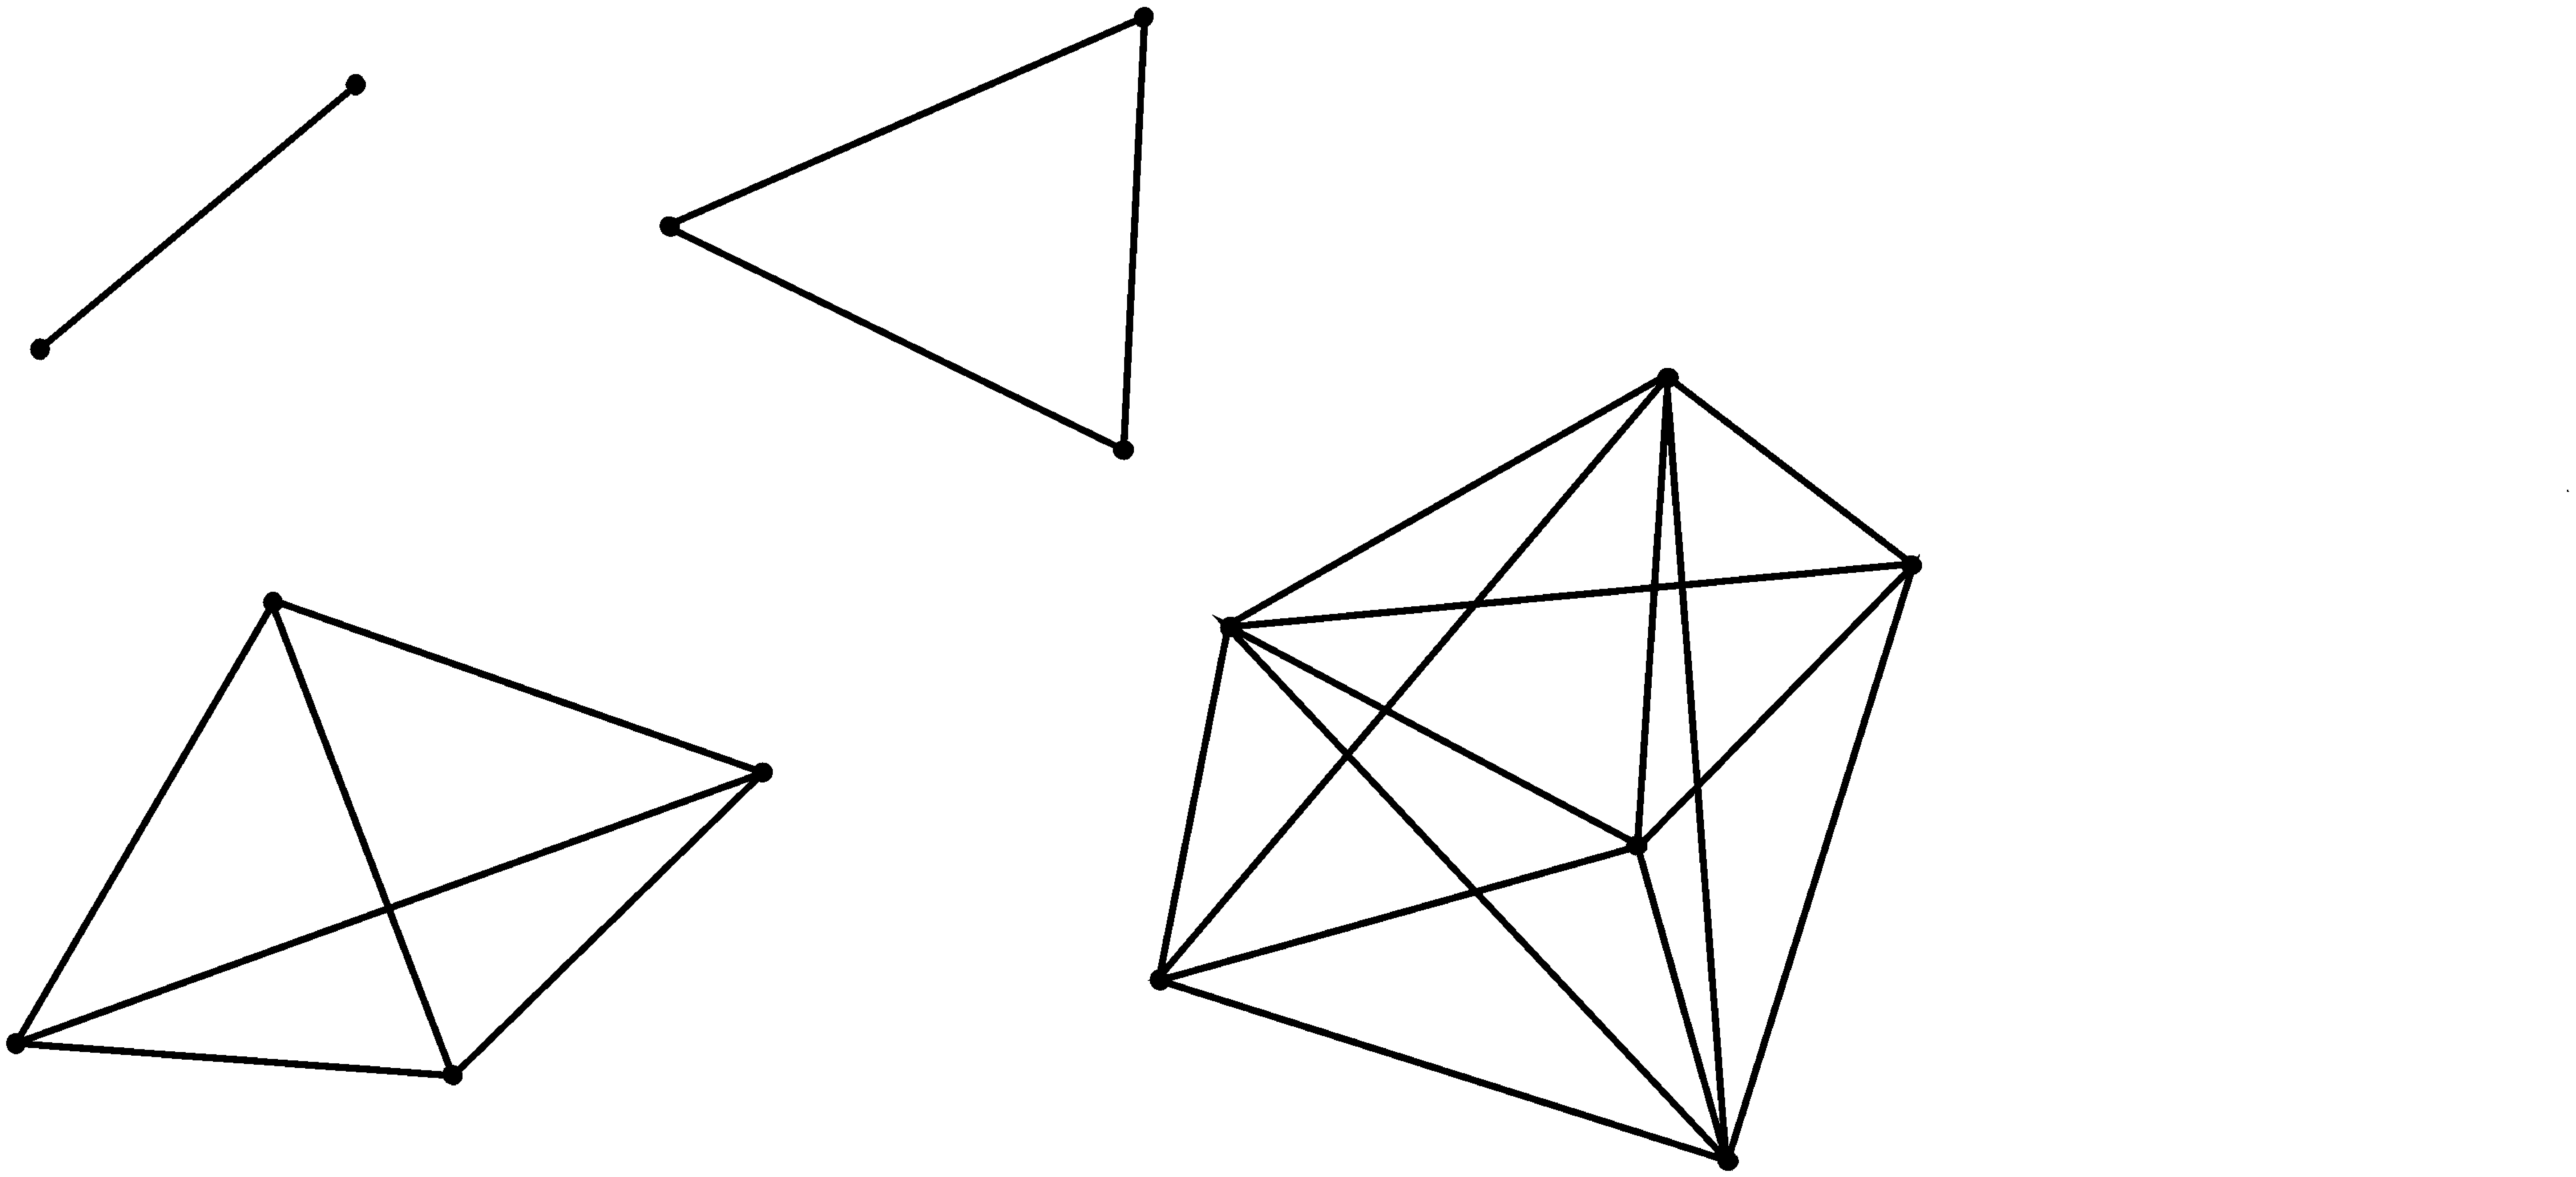
\includegraphics[width=0.6\textwidth]{pict/pict08-2.eps}
\end{center}
 \bigskip
 \refstepcounter{ris}\label{r8-2}

 \centerline{Рис.~\theris}
 \bigskip
\end{figure}

 \vspace{5mm}

Оказывается,
 $$
 \bigcup_{M_n\subset M} \conv M_n=\conv M.
 $$
 Действительно, пусть $x,y$ принадлежат
 $ \bigcup\limits_{M_n\subset M} \conv M_n,$
 тогда $x$ принадлежит некоторому симплексу $\conv M_n,$
 а $y$ принадлежит некоторому симплексу $\conv M_m.$
 Следовательно, $x$ и $y$ принадлежат {симплексу} $\conv M',$ где $M'=M_n
 \bigcup M_m$ и $[x,y]\subset \conv M' \subset
 \bigcup\limits_{M_n\subset M} \conv M_n.$ Таким образом, $\bigcup
 \conv M_n$ выпукло. {Ясно, что это множество} принадлежит любому выпуклому множеству $V,$
 содержащему $M,$ и есть их пересечение.

 \begin{Corollary} %%% Следствие.
 {Множество}
 $$
 \bigcup_{M_n\subset M} \conv M_n
 $$
 есть наименьшее выпуклое множество, содержащее $M.$
 \end{Corollary}

 \begin{Remark} %%% Замечание.
 Если $x_1,\ldots, x_n\subset M,$ то $\conv M_n$ {совпадает с множеством}
 $$
 \left\{x=\sum\limits_{k=1}^n c_kx_k:\quad c_k\ge 0,\quad \sum\limits_{k=1}^n
 c_k=1\right\}.
 $$
 \end{Remark}

Бывает нужна также {\it замкнутая выпуклая оболочка} $\overline{\conv M}$
множества $M.$

\ \

\section{Характеристики линейных нормированных пространств}

{\bf 1.~Сепарабельность}
\vspace{3mm}

Характеристикой массивности пространства является
 наименьшая мощность всюду плотного множества.

 Пространство, для которого существует всюду
 плотное счетное множество, называется {\it сепарабельным}.

 Пространство, не совпадающее с $\theta$ и в котором нет всюду
 плотного счетного множества, называется {\it несепарабельным}.

 Первое, что мы должны проверять для пространства -- сепарабельность.

\vspace{5mm}
{\bf 2.~Полнота}
\vspace{5mm}

Пространство называется {\it полным}, если всякая последовательность
 Коши (фундаментальная последовательность) является сходящейся к
 какому-либо элементу пространства.

 Полное линейное нормированное пространство
 называется {\it банаховым пространством} или пространством
 типа $B.$

\vspace{5mm}
{\bf 3.~Рефлексивность}
\vspace{5mm}

Пусть $X$ -- банахово пространство; $X^*$ -- сопряженное с ним
 пространство линейных непрерывных функционалов, всегда банахово; $X^{**}$ -- второе
 сопряженное пространство.

 Существует каноническое вложение $X$ в $X^{**}$ посредством формулы:
 {для любого} {$x\in X$ положим}
 $$
 F_{{x}}(f)=f(x),\qquad f\in X^*,
 $$
 так что
 $$
 \forall\ x\in X\qquad x\longmapsto F_{{x}}\in X^{**}.
 $$

 Пространство называется {\it рефлексивным}, если при
 каноническом вложении $X$ в $X^{**}$ на самом деле имеем $X\equiv X^{**}$,
 {т.\,е. любой функционал}
 {$F\in X^{**}$ совпадает с некоторым функционалом}
 {$F_x$ над $X^*$.}

 Если пространство рефлексивно, то $X$ и $X^{**}$ устроены одинаково (изоморфны и изометричны).
 Обратно неверно, $X$ и $X^{**}$ могут быть, например, изоморфны, но
 $X$ не рефлексивно.

 Известно, что если  пространство рефлексивно,
 то из любой ограниченной последовательности
 его элементов можно выбрать слабо сходящуюся подпоследовательность.

\vspace{5mm}
 {\bf 4.~Строение сферы (шара)}
 \vspace{5mm}

 {\bf \normalsize   a) Строгая выпуклость.} Пространство называется {\it строго выпуклым},
 если его единичный шар строго выпуклый.

 Единичный шар строго выпуклый, если для любых $x\ne y,$ принадлежащих шару, любая точка
 на интервале $(x,y)$
 лежит строго внутри шара.

 \begin{Example} %%% Пример.
 Круг -- строго выпуклое множество (рис.~8.3), квадрат -- не строго
 выпуклое. Ясно, что если пространство не строго выпуклое,
 то существует гиперплоскость, которая касается единичного
 шара более, чем в одной точке.

 \vspace{0.5cm}
 %%%%%%%%%%%%%%%%%%%%%%%%%%%%%%%%%%%%%%%%%%%%%%%%%%%%%%
 %\hbox to 0.5cm {}{\special{em:graph pict1.pcx}}
 %\vspace{6cm}
 %%%%%%%%%%%%%%%%%%%%%%%%%%%%%%%%%%%%%%%%%%%%%%%%%%%%%%%%%%
 \begin{figure}[ht]
\begin{center}
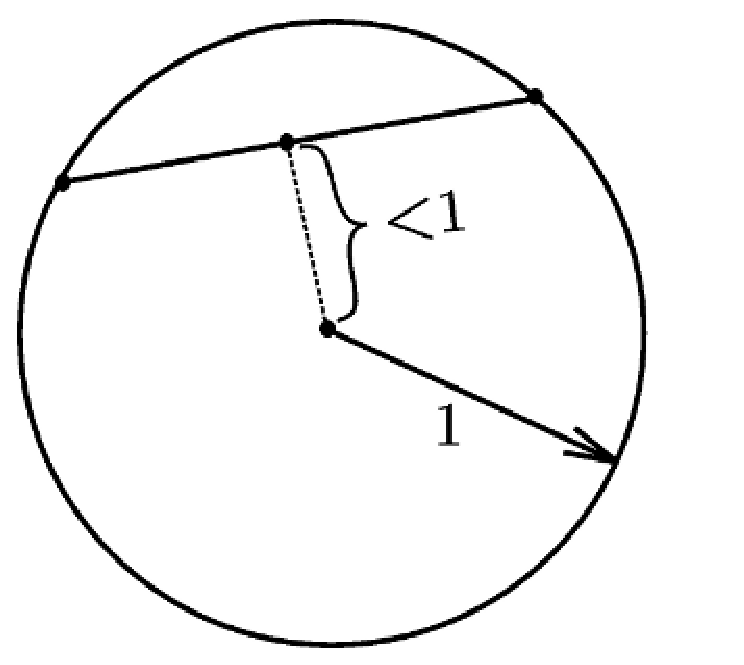
\includegraphics[width=0.3\textwidth]{pict/pict08-3.eps}
\end{center}
 \bigskip
 \refstepcounter{ris}\label{r8-3}

 \centerline{Рис.~\theris}
 \bigskip
\end{figure}
 \end{Example}

 {\bf \normalsize b) Экстремальные точки} {(это линейное понятие).}
 Пусть множество $M\subset X,~ x\in M.$

 Точка $x\in M$ называется {\it неэкстремальной} точкой множества $M,$
 если существуют точки $a,b\in M$ такие, что $x\in (a,b)$
 (рис.~8.4). В противном случае точка называется {\it экстремальной}.

%\newpage

 %\vspace{2cm}
 %%%%%%%%%%%%%%%%%%%%%%%%%%%%%%%%%%%%%%%%%%%%%%%%%%%%%%
 %\hbox to 0.5cm {}{\special{em:graph pict1.pcx}}
 %\vspace{6cm}
 %%%%%%%%%%%%%%%%%%%%%%%%%%%%%%%%%%%%%%%%%%%%%%%%%%%%%%%%%%
   \vspace{10mm}
\begin{figure}[ht]
\begin{center}
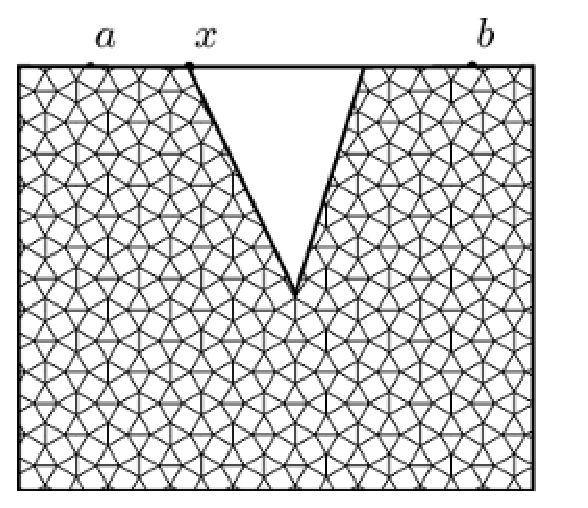
\includegraphics[width=0.3\textwidth]{pict/pict08-4.eps}
\end{center}
 \bigskip
 \refstepcounter{ris}\label{r8-4}

 \centerline{Рис.~\theris}
 \bigskip
\end{figure}

\vspace{5mm}



 Пусть $O_1$ -- единичный шар, $S_1$ -- сфера, его граница.

 {Имеет место}
 \begin{teo}
 В любом конечномерном банаховом пространстве шар $O_1$ есть
 замкнутая выпуклая оболочка своих экстремальных точек.
 \end{teo}

 Теорему приводим без доказательства. В общем случае она неверна. Существуют банаховы
 пространства, в которых единичный шар не имеет
 экстремальных точек.

 \ex
 Доказать, что в единичном шаре $O_1$  в $L{[0,1]}$ нет ни
 одной  экстремальной точки.

 \ex
 Доказать, что шар $O_1$ в $C[0,1]$ имеет две экстремальных точки.

\vspace{5mm}
 {\bf \normalsize c) Гладкость.}
 Пространство называется {\it гладким}, если для любой
 точки на $S_1$ существует единственный опорный функционал,
 т.\,е. единственная касательная гиперплоскости.
 Определение касательной гиперплоскости будет дано позже.

 В противном случае пространство не гладко.

\vspace{5mm}
 {\bf 5.~Компактные множества}
 \vspace{5mm}

  Компактное множество -- такое множество, из любой
 последовательности
 которого можно выбрать сходящуюся подпоследовательность к элементу этого множества.

 Компактное множество всегда замкнуто.

 \vspace{3mm}
 \section{Основные пространства}
  \vspace{3mm}

 {\it Пространство $C=C(Q,X)$ -- это пространство непрерывных функций}, определенных
 на компакте $Q$ и принимающих значения из банахова пространства $X.$
 Классические случаи: $X=\bR,$  $\ X=\bC.$
 \vspace{3mm}

 1. {Пространство $C(Q,X)$} полное.
 \vspace{3mm}

 2. При некоторых $Q$ и $X$ пространство {$C(Q,X)$} сепарабельно, а при некоторых -- нет.

 Если $Q$ -- отрезок, $X=\bR,$ то $C(Q,X)$ сепарабельно.
  \vspace{3mm}

 3. Если $Q$ бесконечно, то $C$ нерефлексивно; в частности, $C[0,1]$ нерефлексивно.
  \vspace{3mm}

 4. {При любых $Q,$ $X$ пространство $C(Q,X)$} не строго выпуклое пространство {и не} {гладкое.}
\vspace{3mm}

 \ex %%%Упражнение.
{Доказать эти свойства.}

{{\it Пространство} $ L^{{p}},~ 1\le p< \infty.$}

 Пусть задано пространство $Q$ с мерой $\mu$ ($\mu$ --
 счетно аддитивная неотрицательная функция измеримых подмножеств из $Q$).

 Пусть $y=f(x)$ -- определенная на $Q$ измеримая
 функция {со значениями в $\bR$ или $\bC$,} для которой
 интеграл  $\ds\int_Q |f(x)|\ d\mu$ конечен, $L_{{\mu}}$ -- множество таких функций и
 $\ds\int_Q |f(x)|\ d\mu=\pnl f\pnr$ -- полунорма.
 Для того, чтобы получить банахово пространство, факторизуем $L_{{\mu}}$:
 $$
  \left. L_{{\mu}} \right/ \{f:\ \pnl f\pnr =0{\}},
  $$
 {т.\,е. будем отождествлять функции, различающиеся лишь на подмножестве нулевой} {меры.}
 Получим полное пространство, которое и далее будем обозначать $L_{{\mu}}.$

 Сепарабельность $L_{{\mu}}$ зависит от $Q$ и от $\mu;$ если $\mu$ --
 мера Лебега на $Q\subset\bR^n,$ то $L_{\mu}=L_{\mu}^1(Q)=L(Q)$ сепарабельно.

 Чтобы получить $L^p_\mu$, возьмем полунорму
 $$
 \pnl f \pnr =\left( \int_Q |f(x)|^p\, d\mu \right)^{1/p}.
 $$
{ Класс эквивалентности, соответствующий функции $f$, будем обозначать тем же}
{символом $f$ и потому $\pnr f\pnr=\|f\|_{L^p}$ -- норма.}

 При $p=2$ получим {$L^2_\mu$} -- гильбертово пространство со скалярным
 произведением
 $$
 (f,g)=\ds\int_Q {fg}\ d\mu
 $$
 над полем действительных чисел,
 $$
 (f,g)=\ds\int_Q {f{\overline g}}\ d\mu
 $$
 над полем комплексных чисел; {$L^2_\mu$}~--
 полное относительно нормы $\|f\|_{{L^2}}=\sqrt{(f,f)}$ {пространство}.

 Напомним, что в пространствах $L^p,\ L^q,$ при $\dfrac{1}{p}+\dfrac{1}{q}=1,\ 1<p,\ q<\infty$
 неравенство Г\"{е}льдера
 $$
 \left| \int_{a}^b f(x)g(x)\,dx\right| \le
 \|f\|_{L^p[a,b]}\|g\|_{L^q[a,b]}
 $$
 для $f\in L^p[a,b],\ g\in L^q[a,b]$ превращается в
 равенство только если $f(x)g(x)\ge 0$ почти всюду и
 $|f(x)|^p$ почти всюду пропорционален $|g(x)|^{q}.$

 \begin{ex}
Рассмотреть эту задачу для функций их $L^p_{\mu}(Q)$ и $L^q_{\mu}(Q).$
 \end{ex}

 \input{lect09.tex}
 % Лекции Сергея Борисовича Стечкина
% ??? Внесены исправления В.И.Бердышева
% Внесены исправления Н.И.Черныха, версия 23.07.2009
% Внесена грамматическая и ТеХ-правка М.Дейкаловой, версия 05.08.09

%%%%%%%%%%%%%%%%%%%%%%%%%%%%%
\chapter{Критерий наилучшего \\
 приближения в $\boldsymbol L^p$. Корректность}
%%% Лекция 10.


 \section{Критерий наилучшего элемента в $L^p$}

  %%% Замечание.
 Пусть $H$ -- гильбертово пространство. В курсе анализа
 доказывается, что для того чтобы $y^*$ был наилучшим элементом в
 подпространстве
 $M\subset H$ для элемента $x,$ необходимо и достаточно, чтобы
 $$
 (x-y^*,y)=0\qquad \forall\  y\in M.
 $$
 Если $H=L_2,$ то это условие можно переписать
 $$
 \int_Q (x-y^*)y\, dt=0\qquad \forall\  y\in M.
 $$


 Оказывается, это утверждение есть частный
 случай более общей теоремы, которая дает необходимое
 и достаточное условие для наилучшего элемента в $L_p,$~ $p>1.$

 \begin{teo} %%% Теорема.
 Пусть $p>1,$~ $M\subset L_p$ -- подпространство, $ \ x\in L_p.$
 Для того, чтобы $y^*$ был наилучшим элементом из $M$ для $x$
 в $L_p$ необходимо и достаточно, чтобы
 \begin{equation}\label{f9-1}
 {\int_Q |x-y^*|^{p-1} \sign (x-y^*)y\, dt=0} {\qquad \forall\  y\in M}.
 \end{equation}
 \end{teo}

 \begin{proof} %%% Доказательство.
 Н\;е\;о\;б\;х\;о\;д\;и\;м\;о\;с\;т\;ь.~ Пусть условие \eqref{f9-1}
 не выполняется, т.\,е. существует $y\in M$ такой, что
 $$
 {\int_Q |x-y^*|^{p-1} \sign (x-y^*)y\, dt\ne 0.}
 $$
 Покажем, что тогда $y^*$ не есть наилучший элемент.

 Рассмотрим
 $$
 \Phi(\alpha)=\|x-y^*-\alpha y\|^p={\int_Q |x-y^*-\alpha y|^p\, dt.}
 $$
 Так как $p>1,$ то это есть дифференцируемая функция от $\alpha,$
 и по теореме о дифференцировании по параметру под
 знаком интеграла
 $$
 \Phi'(\alpha)=-p {\int_Q |x-y^*-\alpha y|^{p-1}\sign(x-y^*-\alpha y)y\, dt.}
 $$
 При $\alpha=0$ имеем $\Phi'(\alpha)|_{\alpha=0}\ne 0,$
 следовательно, при $\alpha=0$ нет минимума. Значит, при некотором
 $\alpha$ можно сделать уклонение $\|x-y^*-\alpha y\|$ еще меньше, чем
 $\|x-y^*\|,$ т.\,е. $y^*$ не является наилучшим элементом. Противоречие.

 Д\;о\;с\;т\;а\;т\;о\;ч\;н\;о\;с\;т\;ь.~ В силу \eqref{f9-1}, применяя неравенство
 Гельдера,  {для любого} {$y \in M$}
 имеем
 $$
 \int_Q |x-y^*|^{p}\, dt=\int_Q |x-y^*|^{p-1}(x-y^*)\sign(x-y^*)\, dt=
 $$
 $$
 =\int_Q |x-y^*|^{p-1}(x-y)\sign(x-y^*)\, dt \le \int_Q |x-y^*|^{p-1}|x-y|\
 dt\le
 $$
 $$
 \le \left\{ \int_Q |x-y^*|^{p}\, dt \right\}^{1/q}\cdot
 \left\{ \int_Q |x-y|^{p}\, dt \right\}^{1/p},\qquad
 {\frac{1}{p}+\frac{1}{q}=1}.
 $$
 Можно считать, что $\ds\int_Q |x-y^*|^{p}\, dt\ne 0$ (в противном случае
 $y^*$ -- наилучший элемент и все доказано). Тогда
 $$
 \left\{ \int_Q |x-y^*|^{p}\, dt \right\}^{1/p}\le
 \left\{ \int_Q |x-y|^{p}\, dt \right\}^{1/p},
 $$
 т.\,е. для любого $y\in M$ выполняется неравенство $\|x-y^*\|\le \|x-y\|,$ значит,
 $\|x-y^*\|=E(x,M).$
 Теорема доказана.
 \end{proof}

 \begin{Remark} %%% Замечание.
 При $p=1$ {условие} \eqref{f9-1} имеет вид
\begin{equation}\label{f9-2}
 \int_Q \sign(x-y^*)y\, dt=0,\qquad \forall\  y\in M,
\end{equation}
 и это есть достаточное условие для того, чтобы $y^*$
 был наилучшим элементом для $x$ (доказательство то же самое).
 Это условие будет и необходимым, если априори известно, что
 $x(t)-y^*(t)\ne 0$ почти всюду на $Q$ (так как тогда при $\alpha=0$ почти всюду существует
 производная $\dfrac{d}{d\alpha}|x-y^*-\alpha y|\Big|_{\alpha=0}=-y
 \, \sign(x-y^*)$). В общем случае это условие только
 достаточное. Необходимое и достаточное условие можно найти
 в работе\footnote{Kripke~B.R., Rivlin~T.J. Approximations in the metric of $L_1(X,\mu)$ //
 Trans. Amer. Math. Soc. 1965. Vol.~119, \No~1, iss.~7.
 P.~101--122.}.
% {[Kripke, Rivlin]}.}
 \end{Remark}

%\vspace{2mm}

%{\bf 1. Наилучшее приближение.}
\section{Наилучшее приближение в $L^1$}

Мы рассмотрели приближение в {$L^p$ подпространствами $M$} и
 доказали, что при $p>1$ {элемент} $y^*\in M$
 будет наилучшим элементом для $x$ тогда и только тогда, когда
 \begin{equation}\label{f9-1-10}
 \int |x-y^*|^{p-1} \sign (x-y^*)y\, dt=0\qquad \forall\  y\in M.
 \end{equation}

 \begin{Example} %%% Пример.
 Рассмотрим частный случай $M=\{c\}$ --  одномерное подпространство
 констант.

 Пусть $p=2$, {$L^p=L^2[a,b].$} В этом случае условие \eqref{f9-1-10} запишется так:
 $$
 \int_{a}^b\{x(t)-c^*\}\, dt=0,
 $$
 т.\,е. (см. рис.~10.1) $S_+=S_-.$

 %\vspace{2cm}
 %%%%%%%%%%%%%%%%%%%%%%%%%%%%%%%%%%%%%%%%%%%%%%%%%%%%%%
 %\hbox to 0.5cm {}{\special{em:graph pict1.pcx}}
 %\vspace{6cm}
 %%%%%%%%%%%%%%%%%%%%%%%%%%%%%%%%%%%%%%%%%%%%%%%%%%%%%%%%%%
 %\noindent \hskip3.0cm {рис.}

  \bigskip
\begin{figure}[ht]
\begin{center}
\includegraphics{pict/pict10-1.eps}
\end{center}
 \bigskip
 \refstepcounter{ris}\label{r10-1}

 \centerline{Рис.~\theris}
 \bigskip
\end{figure}



 \noindent Если $p=1,$ то условие \eqref{f9-1-10} перепишется как
 $$
 \int_a^b\sign \{x(t)-c^*\}\, dt=0
 $$
 или, { в случае, когда $L^1[a,b]$ есть пространство с мерой $\mu,$ как}
 \begin{equation}\label{f10-1}
 \mu(E_+)-\mu(E_-)=0,
 \end{equation}
 где $E_+\ (E_-)$ -- множество, на котором разность $x(t)-c^*>0\
 (<0),$~ $\mu$ -- мера.
 \end{Example}

 Легко построить пример, когда нет единственности
 наилучшего элемента в {$L^1$} \linebreak {{(см. рис.~10.2)}:}

\begin{figure}[ht]
\begin{center}
\includegraphics[width=0.5\textwidth]{pict/pict10-2.eps}
\end{center}
 \bigskip
 \refstepcounter{ris}\label{r10-2}

 \centerline{Рис.~\theris\ \  $(c^*\in [0,1])$}
\end{figure}



 \noindent Любая константа $c^*\in [0,1]$ -- {здесь} наилучшая.

 Как отмечалось, при $p=1$ {условие} \eqref{f9-1-10} -- {только} достаточное для наилучшего
 элемента. Можно построить пример, когда для наилучшей
 константы в {пространстве $L^1$ с мерой} условие \eqref{f10-1} {тоже} не выполняется
 (см. рис.~10.3 для меры Лебега).

 %\vspace{2cm}
 %%%%%%%%%%%%%%%%%%%%%%%%%%%%%%%%%%%%%%%%%%%%%%%%%%%%%%
 %\hbox to 0.5cm {}{\special{em:graph pict1.pcx}}
 %\vspace{6cm}
 %%%%%%%%%%%%%%%%%%%%%%%%%%%%%%%%%%%%%%%%%%%%%%%%%%%%%%%%%%
 %\noindent \hskip3.0cm {рис.}
 \bigskip
\begin{figure}[ht]
\begin{center}
\includegraphics{pict/pict10-3.eps}
\end{center}
 \bigskip
 \refstepcounter{ris}\label{r10-3}

 \centerline{Рис.~\theris\ (здесь видно, что $c^*=1/2$)}
 \bigskip
\end{figure}




 Если {же $\mu\{t\in[a,b] : x(t)-y^*(t)=0\}=0,$} то дифференцирование под знаком интеграла
 законно, и нарушение условия \eqref{f10-1} означает, что $y^*$ не является наилучшим
 элементов в $M$ для $x$.

 Пусть $X$ -- банахово пространство, $M\subset X $ --
 подпространство.
 В задаче о наилучшем приближении для любого $x\in X$
 мы ищем $y^*\in M$ такой, что
 $$
 \|x-y^*\|_X\le \|x-y^*-h\|\qquad \forall\  h\in M;
 $$
 т.\,е. $y^*$ будет наилучшим элементом, если  не найдется понижающий
 элемент $h.$ Значит, функционал
 $$
 \Phi(h)=\|x-y^*-h\|
 $$
 должен достигать при $h=\theta$ своего минимума. Если $\Phi(h)$ --
 дифференцируемый функционал, то для минимума необходимо, чтобы
 дифференциал от $\Phi(h)$ обращался в 0 при $h=\theta.$
 Или пусть фиксировано $h.$ Тогда функционал
 $$
 F_h(t)=\|x-y^*-th\|,\qquad t\in (-1,1),
 $$
 должен иметь минимум в точке $t=0$ при каждом $h\in M$; т.\,е. $\cD\|x-y^*-h\|
 |_{h=\theta}=0,$ так что условие \eqref{f9-1-10} просто означает, что дифференциал равен
 нулю.

 Так как $\Phi(h)$ -- выпуклый функционал, то
если $\Phi(h)$~-- дифференцируемый функционал,
 условие обращения дифференциала для $\Phi(h)=\|x-y^*-h\|$ на пространстве
 $M$ в 0 при $h=\theta$ есть необходимое и достаточное для того, чтобы $y^*$
 был наилучшим.

\section{Корректность}

Рассмотрим вопрос о непрерывной зависимости решения задачи наилучшего приближения
от задаваемых условий.

 Пусть $X$ --~банахово пространство, и пусть далее $M\subset X$ --~множество
 существования, элементы $x\in X,$ $y(x)$ -- элемент
 наилучшего приближения в $M$ для $x$, $E(x,M)_X$ --~наилучшее приближение
 элемента $x.$ Очевидно, что $E(x,M)_X=\Phi(x)$ --
 функционал~от~$x.$

 Так как
 $$
 E(x,M)-E(x',M)=\|x-y(x)\|-\|x'-y(x')\|\le \|x-y(x')\|-\|x'-y(x')\|\le
 \|x-x'\|,
 $$
 то получаем, что {\it наилучшее приближение {$E(x,M)$} зависит от} $x$
 {\it {непрерывно и} {даже равномерно непрерывно.}}

\ex Доказать полученную оценку без предположения $M\in (E).$

 Пусть теперь в $M$ и для $x$, и для $x'$ существуют единственные
 наилучшие элементы $y(x)$ и $y(x').$ Если $x$ и $x'$ близки,
 следует ли тогда, что $y(x)$ и $y(x')$ близки? Вообще говоря, это не
 так, $y(x),$ вообще говоря, не является непрерывной функцией от $x.$
 Но непрерывность $y(x)$ имеет место в одном важном случае.

 Пусть $M$ ограниченно компактно, т.\,е. пересечение $M$
 с любым шаром {есть} компакт. Ограниченно компактное
 множество всегда есть множество существования, т.\,е.
 для любого $x$ множество наилучших элементов
 $Y(x)\subset M$ не пусто. {Нас интересует} {непрерывность отображения}
 $$
   x \longmapsto Y(x)\subset M,\qquad{ x \in X}.
 $$
 Будем рассматривать {$Y_{\varepsilon}$~--} $\varepsilon$-расширение $Y(x)$ в $M$,~
 {$Y_{\varepsilon}=\{y\in M:\rho(y,Y(x))<\varepsilon\}$}
 Зафиксируем какой-нибудь элемент $x\in X.$
 Выясним, как связаны $Y_{\varepsilon}$ и $Y.$

 %\vspace{2cm}
 %%%%%%%%%%%%%%%%%%%%%%%%%%%%%%%%%%%%%%%%%%%%%%%%%%%%%%
 %\hbox to 0.5cm {}{\special{em:graph pict1.pcx}}
 %\vspace{6cm}
 %%%%%%%%%%%%%%%%%%%%%%%%%%%%%%%%%%%%%%%%%%%%%%%%%%%%%%%%%%
 %\noindent \hskip3.0cm {рис.}

  \bigskip
\begin{figure}[ht]
\begin{center}
\includegraphics{pict/pict10-4.eps}
\end{center}
 \bigskip
 \refstepcounter{ris}\label{r10-4}

 \centerline{Рис.~\theris}
 \bigskip
\end{figure}



 \noindent Ясно, что $Y=\bigcap\limits_{\varepsilon >0} Y_{\varepsilon}.$
 Теперь возьмем $E(x,M)=d$ и рассмотрим множество\linebreak (см. рис.~10.4)
 $$
 Z(\varepsilon)=Z(\varepsilon,x)=\{ z\in M:\ \|x-z\|\le d+\varepsilon\}.
 $$
 Тогда для ограниченно компактных множеств $M$ справедливо

 \begin{Proposition} %%% Утверждение.
 Для любого $\varepsilon>0$ найдется $\varepsilon_1>0$ такое, что
 $Z(\varepsilon_1)\subset Y_\varepsilon.$
 \end{Proposition}

 Действительно, {$\{Z(\varepsilon_1)\}_{\varepsilon_1}$} --
 убывающая по вложению при $\varepsilon_1\downarrow 0$
 система компактных множеств и $\bigcap\limits_{\varepsilon_1>0} Z(\varepsilon_1)=Y{(x)}.$
 Тогда по свойству компактных множеств для любой окрестности
 $Y_{\varepsilon}$  {множества $Y(x)$}
 все $Z(\varepsilon_1),$ начиная
 с некоторого $\varepsilon_0,$ т.\,е. при $\varepsilon_1\le \varepsilon_0,$
 лежат внутри $Y_{\varepsilon}.$

 В общем случае, если нет ограниченной компактности, это утверждение
 не имеет места.

 В частности получаем, что если
 {в ограниченно компактном множестве $M$}
 есть единственный
 наилучший элемент
{для $x$}, то все <<хорошие>> точки, т.\,е. такие $z\in M,$
 расстояние от которых до $x$
 мало отличается от наилучшего приближения, лежат
 в некоторой малой окрестности наилучшего элемента.

 \begin{teo}[о корректности] %%% Теорема
 Пусть $X$ -- банахово пространство, $M$ -- ограниченно компактное
 подмножество из $X,$~ $x\in X$ и существует единственный элемент
 $y^*\in M,$ ближайший к {$x.$} Тогда если $\{x_n\}$ -- любая сходящаяся
 к $x$ последовательность из $X$ и $\{y_n\}$ -- последовательность из
 $M$ такая, что $\|x_n-y_n\|\to \|x-y^*\|,$ то $y_n\to y^*.$
 \end{teo}

 Действительно, для любого $\delta>0$ для достаточно
 больших $n$
 $$
 \|x-y_n\|\le \|x-x_n\|+\|x_n-y_n\|\le \|x-y^*\|+\delta,
 $$
 т.\,е. $y_n\in Z(\delta).$ Мы уже отмечали, что для любого
 $\varepsilon>0$ множество $Z(\delta)$ принадлежит $Y_{\varepsilon}$ для
 достаточно малых $\delta.$ Таким образом, $\|y_n-y^*\|\le \varepsilon$
 для всех достаточно больших $n,$ т.\,е. $y_n\to y^*.$

 Учитывая непрерывность $E(x,M)$ {получаем}
 \begin{Corollary}
 Пусть $M$ -- ограниченно компактное множество из $X$
 и для любого $x\in X$ наилучший элемент $y(x)$ -- единственный.
 Тогда $y(x)$ {есть} непрерывная функция от $x$
 на всем банаховом пространстве. {При этом} $y(x)$ будет равномерно непрерывной
 функцией, если $x\in K,$ где $K$ -- компакт.
 \end{Corollary}

 \task %%% Задача.
 В пространстве $C{=C[0,1]}$ приближаем функциями из класса
 $$
 \{ x\in C:\quad \|x'\|\le 1,\quad x(0)=0\}.
 $$
 Будет ли $y(x)$ непрерывна? В каких банаховых пространствах для
 любого подпространства {$M$ метрическая проекция $y(x)$}
 равномерно непрерывна?

 Пусть $H$ -- гильбертово пространство, $M\subset H $ -- подпространство,
 $  x\in X,$ $y(x)$~{-- ближайший к $x$ элемент в $M.$}
 Из критерия наилучшего приближения
 $$
 (x-y(x),y)=0\qquad \forall\  y\in M
 $$
 следует, что
 $$
 \|x-y(x)\|^{2}+\|y(x)\|^2=\|x\|^2
 $$
 и
 $$
 \|y(x)\|\le \|x\|.
 $$
 Тогда {в силу линейности метрической проекции в $H$ на подпространство}
 $$
 \|y(x)-y(x')\|=\|y(x-x')\|\le \|x-x'\|,
 $$
 т.\,е. метрическая проекция в гильбертовом
 пространстве равномерно непрерывна (и является
 ограниченным линейным оператором).

 \begin{Remark} %% Замечание.
 Вообще говоря (и как правило, если пространство не гильбертово), линейность наилучших
 элементов не имеет места. Например, пусть в $C[-1,1]$
 приближаем константами {(см. рис.~10.5)} функции
 $$
     {f_1(t)=\begin{cases}
     0, & -1 \le t \le 0 \\
     t, & 0 < t \le 1
   \end{cases},}
   $$
   $$
   f_2(t)=f_1(-t),
   \qquad (f_1+f_2)(t)=|t|.
 $$

 %\vspace{2cm}
 %%%%%%%%%%%%%%%%%%%%%%%%%%%%%%%%%%%%%%%%%%%%%%%%%%%%%%
 %\hbox to 0.5cm {}{\special{em:graph pict1.pcx}}
 %\vspace{6cm}
 %%%%%%%%%%%%%%%%%%%%%%%%%%%%%%%%%%%%%%%%%%%%%%%%%%%%%%%%%%
 %\noindent \hskip3.0cm {рис.}

 \bigskip
\begin{figure}[ht]
\begin{center}
\includegraphics{pict/pict10-5.eps}
\end{center}
 \bigskip
 \refstepcounter{ris}\label{r10-5}

 \centerline{Рис.~\theris}
 \bigskip
\end{figure}

 \noindent Здесь имеем: $\dfrac12=c^*(f_1)=c^*(f_2)=c^*(f_1+f_2)\ne c^*(f_1)+
 c^*(f_2)=1.$

 Линейность имеет место только в гильбертовом
 и некоторых вырожденных пространствах.
 \end{Remark}

 \begin{teo} %%% Теорема.
 Пусть $X$ -- равномерно выпуклое пространство, $M\subset X $ -- подпространство. Тогда $M$
 -- подпространство единственности, и метрическая проекция $y(x)$ {на $M$}
 равномерно непрерывно зависит от $x$ {на любом ограниченном} {множестве}.
 \end{teo}

 \begin{proof} %%% Доказательство.
 Первое утверждение теоремы вытекает из теоремы~9.3.
 Применяя неравенство треугольника
 и используя свойства наилучшего приближения, для произвольных элементов $x$ и $x',$
 обладающих наилучшими элементами в $M,$ получаем
 $$
 \|x-y(x{'})\|\le \|x'-y(x')\|+\|x-x'\|\le \|x'-y(x)\|+\|x-x'\|\le
 $$
 $$
 \le \|x-y(x)\|+\|x-x'\|+\|x-x'\|=\|x-y(x)\|+2\|x-x'\|,
 $$
 т.\,е. если $x'$ близок к $x,$ то равномерно относительно $x$ и $x'$ элемент
 $y(x')$ имеет отклонение от $x$, {близкое к наилучшему.} Получили, что
 $y(x')\in Z(2\|x-x'\|,x).$
 Ввиду равномерной выпуклости пространства отсюда
 следует, что расстояние между $y(x)$ и $y(x')$
 равномерно уменьшается с уменьшением расстояния между $x$ и $x'$
при условии, что величины $\|x\|$ ограничены.

 Пространства $L_p,~ p>1,$ равномерно выпуклы, следовательно, в $L_p,~
 p>1,$
 {на} {ограниченном множестве элементов метрическая проекция}
 $y(x)$ равномерно непрерывна.

 В гильбертовом пространстве, как уже отмечали,
 метрическая проекция равномерно непрерывна {на всем пространстве}.

 В пространстве $C{[a,b]}$ метрическая проекция не является равномерно
 непрерывной.
 \end{proof}

 \begin{Example} %%% Пример.
 В $C[0,1]$ приближаем функциями $a+bx=p(x).$ Построим для любого
 $\varepsilon>0$ непрерывные на $[0,1]$ функции $f$ и $\widetilde f$
 такие, что $\|f-{\widetilde f}\|_C\le \varepsilon,$ но
 $\|p^*(f)-p^*({\widetilde f})\| {> 1}.$
 Это и будет означать, что для метрической проекции $p(f)$
 нет равномерной непрерывности. Пример называется <<молния>> (см. рис.~10.6).
 Здесь $\widetilde f(\varepsilon)=1+\varepsilon,~ \widetilde f(-\varepsilon)=1-\varepsilon,$
 $f(-1)=\widetilde{f}(-1)=0,\ f(1)=\widetilde{f}(1)=0,\ f(0)=\widetilde{f}(0)=-1,\
 f(\varepsilon)=f(-\varepsilon)=1,\ \widetilde{f}(-\varepsilon)=1-\varepsilon,\
 \widetilde{f}(\varepsilon)=1+\varepsilon$~-- вершины
 ломанных -- графиков функций $f(x)$ и $\widetilde{f}(x).$

 %\vspace{2cm}
 %%%%%%%%%%%%%%%%%%%%%%%%%%%%%%%%%%%%%%%%%%%%%%%%%%%%%%
 %\hbox to 0.5cm {}{\special{em:graph pict1.pcx}}
 %\vspace{6cm}
 %%%%%%%%%%%%%%%%%%%%%%%%%%%%%%%%%%%%%%%%%%%%%%%%%%%%%%%%%%
 %\noindent \hskip3.0cm {рис.}

 \bigskip
\begin{figure}[ht]
\begin{center}
\includegraphics{pict/pict10-6.eps}
\end{center}
 \bigskip
 \refstepcounter{ris}\label{r10-6}

 \centerline{Рис.~\theris}
 \bigskip
\end{figure}


 \noindent Здесь наилучшим для $f$ является $p^*(f)\equiv 0,$
 наилучшим для $\widetilde f$ является $p^*(\widetilde f\,)=x,$
 это следует из теоремы Чебышева об альтернансе
 (будет доказана). В примере есть чебышевские
 альтернансы необходимой длины.
 \end{Example}

 \begin{Example} %%% Пример.
В $C[0,1]$ будем приближать функции рациональными дробями из множества
 $$
 M=\left\{ \frac{a}{b+cx}\right\}
 $$
 Можно показать, что оператор наилучшего приближения в этом случае не является непрерывным.

 Действительно, используя критерий Чебышева, для каждого $r>0$ легко построить
 непрерывную функцию $f_r,$ для которой $\dfrac{1}{1+rx}$
 будет наилучшей рациональной дробью (по чебышевскому
 альтернансу в трех точках)
 и такую, что $f_r(x) \rightrightarrows f,$ причем
 для $f$ наилучшая рациональная дробь тождественно равна $0,$ а $\dfrac{1}{1+rx}
 \not\rightrightarrows 0$~ $(r\to \infty),$ так как
 функция $R(x),$ предельная для последней дроби, является разрывной на
 отрезке $[0,1]$: $R(0)=1,\ R(x)=0,\ 0< x\le 1.$

 Таким образом, оператор {наилучшего} проектирования в $C[0,1]$ на {множество} гипербол терпит
 разрыв (см. рис.~\ref{r10-7}).
 \end{Example}

 %\vspace{-5cm}
\begin{figure}[h]
\begin{center}
\includegraphics[width=0.5\textwidth]{pict/pict10-7.eps}
\end{center}
\bigskip
\refstepcounter{ris}\label{r10-7}

\centerline{Рис.~\theris}
\end{figure}

\begin{ex}
 Придумать метрику в трехмерном пространстве (<<шар>>, определяющий
 метрику) такую, чтобы метрическая проекция на некоторое
 одномерное подпространство была разрывной.
\end{ex}

 \input{lect11.tex}
 % Лекции Сергея Борисовича Стечкина
% ??? Внесены исправления С.В. Конягина и И.Г. Царькова, версия 24.02.2009
% Внесены исправления Н.И. Черныха, версия 16.07.2009
% Внесена грамматическая и ТеХ-правка М.Дейкаловой, версия 05.08.09

\chapter{Системы Чебышева. Теорема Хаара}

\section{Чебышевские подпространства в $C(K)$}

Изучаем приближения действительных функций в метрике $C$ посредством
конечномерных подпространств.

Пусть $f\in C[a,b]$,~ $L_n\subset C[a,b]$ --
подпространство, порожденное системой линейно независимых функций
$(\varphi) = \{\varphi_1,\ldots,\varphi_n\}$;
ищем наилучший
полином $\varphi^*(f)$ по системе $(\varphi)$, т.\,е. полином,
на котором достигается $E(f,L_n)_C.$ Было доказано, что если $(\varphi)$
не является системой Чебышева, то найдется элемент из
$C[a,b]$, для которого наилучшее приближение не единственно.

\begin{task}
(Не исследована до конца). На каких компактных множествах $K$ существуют
векторнозначные системы Чебышева, принимающие значения в $\mathbb R^m$?
\end{task}

Для случая $m=1$ имеется теорема Мейерхьюбера: для того, чтобы на
компакте существовала система Чебышева длины больше 1, необходимо и достаточно,
чтобы компакт был гомеоморфен части окружности, а при $n$ четном --
ее собственной части.

\begin{teo}[А.\,Хаар]
Пусть $K$ -- компакт. Для того, чтобы линейно независимая система {$(\varphi)$}
порождала чебышевское подпространство
{в $C(K)$}, необходимо и достаточно, чтобы она была системой
Чебышева на $K$.
\end{teo}

\begin{proof}
Н\;е\;о\;б\;х\;о\;д\;и\;м\;о\;с\;т\;ь~ обсуждалась на прошлой лекции:
именно, было доказано (для $K=[a,b]$), что если система нечебышевская, то
найдется функция, для которой наилучший полином не единственен.

Д\;о\;с\;т\;а\;т\;о\;ч\;н\;о\;с\;т\;ь.~ Пусть $C(K)$~-- множество
непрерывных функций на компакте $K,$ и система функций $(\varphi) =
\{\varphi_1,\ldots,\varphi_n\}$~-- чебышевская. Покажем, что тогда
она является системой единственности. В силу линейной
независимости системы $(\varphi)$ для
мощности $K^\sharp$ компакта справедлива оценка $K^\sharp\ge
n.$ Если $K^{\sharp}=n,$ то пространство, порожденное
системой $(\varphi)$ совпадает с $C(K),$ и значит, является
чебышевским.

Пусть $f\in C(K)$,~ $\varphi(x)=\sum\limits_{k=1}^n a_k \varphi_k(x)$~
($x\in K$)~-- произвольный полином по заданной системе функций.
Рассмотрим \textit{множество точек максимального уклонения}
$$
M(f,\varphi) = \{x\in K\colon \|f-\varphi\|_C=|f(x)-\varphi(x)|\}.
$$
Так как $K$~-- компакт и $f$ и $\varphi$~-- непрерывные функции, то такое множество непусто.

Пусть теперь $\varphi^*$ -- наилучший полином для $f$, т.\,е.
$\|\varphi^*-f\|=E(f,{L_n})_C$. Будем изучать $M(f,\varphi^*)$. Докажем
вспомогательное

\begin{Proposition}\label{card_M}
Пусть $f\in C(K)$, и $\varphi^*$ -- ее наилучший полином по
чебышевской системе порядка $n.$ Тогда множество $M(f,\varphi^*)$ не может
быть слишком маленьким, а именно, должно быть
$$
\card M(f,\varphi^*)\ge n+1.
$$
\end{Proposition}

Докажем это утверждение от противного. Пусть для некоторых $f$ и
$\varphi$ число точек в $M(f,\varphi)$
не превышает $n$. В частности, тогда $f\notin L_n,\ E_n(f,L_n)_C>0.$
Покажем, что такой полином $\varphi$ не является наилучшим.

Построим понижающий полином $h\in (\varphi)$ такой, что $\varphi+\eps h$
дает меньшее уклонение от $f$:
$$ \|f-(\varphi+\eps h)\|<\|f-\varphi\| $$
для некоторого $\eps > 0$. Рассмотрим множество $M(f,\varphi)$. Оно состоит
из точек $x_1,\ldots,x_n$ (если точек $\{x_k\}$ меньше чем $n$,
доказательство такое же). {В силу свойства} {интерполяционности
системы $(\varphi)$ существует} полином $h$ такой, что {для всех $x_k$}
$$
h(x_k) = f(x_k)-\varphi(x_k){(\ne 0)}.
$$
Окружим точки $x_k$ окрестностями $U_k$, в которых функции $h$ и $f-\varphi$
сохраняют знак. Тогда $|f-\varphi-\eps h|<\|f-\varphi\|$ в $U_k$
при малых $\eps>0$. Вне объединения $U_k$ имеем $|f-\varphi|<\|f-\phi\|_C$.
{Значит,} $|f-\varphi-\eps h| < \|f-\varphi\|_C$ при достаточно
малых $\eps$. Утверждение доказано.

Вернемся к доказательству теоремы Хаара (от противного). Пусть есть функция
$f\in C(K)$ и для нее имеется два наилучших полинома $\varphi_1^*$ и
$\varphi_2^*$:
$$
\|f-\varphi_1^*\|=\|f-\varphi_2^*\|=E(f,{L_n})_C=E.
$$
Тогда, так как множество наилучших полиномов выпукло, то при
любом $t\in[0,1]$ для $\varphi = t\varphi_1^* + (1-t)\varphi_2^*$ справедливо
равенство $\|f-\varphi\|=E$. В частности, при $t=\dfrac12$
полином $\widetilde\varphi = \dfrac12\,\varphi_1^*+\dfrac12\,\varphi_2^*$~--
наилучший, и по доказанному утверждению найдутся точки $x_k$,~ $k=1,2,\ldots,n+1$, в которых
$$
\|f-\widetilde\varphi\|=|f(x_k)-\widetilde\varphi(x_k)|=E.
$$
В этих точках для $\varphi_1^*$ и $\varphi_2^*$ должно быть
$$
|f(x_k)-\varphi_1^*(x_k)|=E,\qquad |f(x_k)-\varphi_2^*(x_k)|=E,
$$
причем знаки разностей должны быть одинаковы, т.\,е.
$$
f(x_k)-\varphi_1^*(x_k) = f(x_k)-\varphi_2^*(x_k) = \pm E.
$$
Отсюда следует, что для полинома $h=\varphi_1^*-\varphi_2^*$, не равного
тождественно нулю по предположению,
$$
h(x_k) = \varphi_1^*(x_k)-\varphi_2^*(x_k) = (f(x_k)-\varphi_2^*(x_k))-
(f(x_k)-\varphi_1^*(x_k)) = 0,\qquad k=1,\ldots,n+1.
$$
Таким образом, ненулевой полином по системе Чебышева имеет $n+1$ нуль,
чего не может быть. Значит, $h\equiv 0$~-- противоречие. Теорема
доказана.
\end{proof}

\begin{Remark}
Условие $\card M(f,\varphi^*)\ge n+1$ для наилучшего полинома $\varphi^*$~-- необходимое, но не достаточное.
\end{Remark}

\begin{Example}
В $C[0,1]$ приближаем константами, $n=1$,~ $n+1=2$. Для наилучшей константы
$\varphi^*=\dfrac12$ (см. рис.~\ref{r12-1})
$$
\card M(f,\varphi)\ge n+1=2.
$$

 \bigskip
\begin{figure}[ht]
\begin{center}
\includegraphics{pict/pict12-1.eps}
\end{center}
 \bigskip
 \refstepcounter{ris}\label{r12-1}

 \centerline{Рис.~\theris}
 \bigskip
\end{figure}


%константы
Для любой постоянной функции $\varphi<\dfrac12$ имеется континуум точек
максимального уклонения, но она не есть наилучшая.
\end{Example}


\section{Теорема Чебышева}

Пусть $f$~-- непрерывная на $[a,b]$ функция, $(\varphi)$~-- система Чебышева
и $\varphi=\sum\limits_{k=1}^n a_k \varphi_k(x)$~-- полином по этой
системе.

Рассмотрим множество $M=M(f,\varphi)$ точек максимального уклонения.

Будем говорить, что $M(f,\varphi)$ имеет (чебышевский) альтернанс длины $n+1$,
если существуют точки $x_1, x_2,\ldots,x_{n+1}$ из $M$ такие, что

1) $a\le x_1<x_2<\ldots<x_{n+1}\le b$,

2) знаки разностей $f(x_k)-\varphi(x_k)$ чередуются
($k=1,2,\ldots,n+1$).

\begin{teo}[П.\,Л.\,Чебышев]
Для того, чтобы полином $\varphi$ по чебышевской системе порядка $n$ на отрезке был
наименее уклоняющимся от $f$, необходимо и достаточно, чтобы
множество точек максимального уклонения $M(f,\varphi)$ имело альтернанс длины
по крайней мере $n+1$.
\end{teo}

\begin{proof}
Н\;е\;о\;б\;х\;о\;д\;и\;м\;о\;с\;т\;ь.~ Пусть в $M(f,\varphi)$ не
содержится альтернанс длины $n+1$. Покажем, что тогда найдется полином с
меньшим уклонением.

Пусть $M(f,\varphi) = M_+\cup M_-$, где
$$
M_+=\{x\in M(f,\varphi)\colon f(x)-\varphi(x)>0\},\qquad
M_-=\{x\in M(f,\varphi)\colon f(x)-\varphi(x)<0\}.
$$
{Можно считать также,
что $M_+\ne \varnothing$ и $M_-\ne \varnothing$, так как в противном случае найдется}
{полином $\varphi(x)-\varepsilon P_+(x)$ с меньшим уклонением, где
$P_+(x)>0$ на $[a,b]$,~ $\varepsilon>0$ при} {$M_+\ne \varnothing$,
$\varepsilon<0$ при $M_-\ne \varnothing$ и $|\varepsilon|$ -- достаточно
малое число. Существование полинома} {$P_+(x)$ по чебышевской системе было
доказано ранее.} Пусть также $\eta_1=\min\{x\colon x\in M(f,\varphi)\}$;
без ограничения общности предполагаем, что $\eta_1\in M_+$. Обозначим
$$ \eta_2 = \min\{x>\eta_1\colon x\in M_-\}, $$
$$ \eta_3 = \min\{x>\eta_2\colon x\in M_+\} $$
и т.\,д. Мы получили систему точек $\eta_1<\ldots<\eta_k$; при этом по
{нашим предположениям} {$1<k\le n$}. Далее, положим
$$ \zeta_1 = \max\{x\in M_+\colon x<\eta_2\}, $$
$$ \zeta_2 = \max\{x\in M_-\colon x<\eta_3\}, $$
$$ {\ldots\ldots\ldots\ldots\ldots\ldots\ldots\ldots\ldots} $$
$$ {\zeta_k = \max\{x\in M\} \qquad (\zeta_k\ge\eta_k).} $$


Наконец, на каждом интервале $(\zeta_i,\eta_{i+1})$,~ $i=1,\ldots,k-1$,
возьмем произвольным образом точку $\xi_i$.

Окружим отрезки $[\eta_i,\zeta_i]$, {$i=1,\ldots,k$}, интервалами {$(a_i,b_i)$},
не содержащими точек~$\xi_i$ (см. рис.~\ref{r12-2}). В случае $\eta_1=a$
и/или $\zeta_k=b$ вместо $(a_1,b_1)$,~ $(a_k,b_k)$ возьмем промежутки $[a,b_1)$,
$(a_k,b]$. По доказанному ранее, если $k=n$, то существует
полином $h(x)=\pm{\cal D}(x;\xi_1,\ldots,\xi_{n-1})$,
который в точках $\xi_1,\ldots,\xi_{n-1}$ имеет нули и меняет знаки.

 \bigskip
\begin{figure}[ht]
\begin{center}
\includegraphics{pict/pict12-2.eps}
\end{center}
 \bigskip
 \refstepcounter{ris}\label{r12-2}

 \centerline{Рис.~\theris}
 \bigskip
\end{figure}


Правильно выбрав знак в формуле для $h(x),$ можно считать, что $h(x)>0$ на интервалах
{$(a_{2i-1},b_{2i-1})$} и $h(x)<0$ на интервалах $(a_{2i},b_{2i})$.
{Если же $k<n$, то
недостающие различные точки $\{\xi_i\}_{i=k}^{n-1}$ поместим в случае
четного их числа на интервале $(\xi_1,a_2)$, а в случае нечетности $n-k$
возьмем $\xi_{n-1}=a$ при $a<\eta_1$ или $\xi_{n-1}=b$ при $\zeta_k<b$,
а остальные точки $\{\xi_i\}_{i=k}^{n-2}$ разместим так же на интервале
$(\xi_1,a_2).$ Ясно, что построенный по этим точкам полином $h(x)$
сохраняет свойство $\sign h(x)=\sign(f(x)-\varphi(x))$ при $x\in(a_i,b_i)\cap M,\
(i=1,2,\ldots,k)$, уже доказанное в случае $k=n.$
Осталось построить такой же полином в оставшемся
случае, когда $n-k$ нечетно и $\eta_1=a,$~ $\zeta_k=b.$ В этом случае по уже
выбранным точкам $\{\xi_k\}_{k=1}^{n-2}$ построим два полинома
$h_a(x)$ и $h_b(x),$ зануляющихся в них и в точках $x=a,$~ $x=b,$ соответственно.
Полагая $h=h_a+h_b$, опять получим полином с нужными свойствами.}
Рассуждая далее как в конце доказательства утверждения~\ref{card_M}, видим, что
$\|f-\varphi-\eps h\|<\|f-\varphi\|$ при малых $\eps>0$.

Д\;о\;с\;т\;а\;т\;о\;ч\;н\;о\;с\;т\;ь.~ Предположим, что имеется альтернанс длины
$n+1$. Покажем, что тогда $\varphi$ есть полином, наименее
уклоняющийся от функции $f$. Если это не так и существует еще один полином
$\varphi_1$, который дает меньшее уклонение, то в точках альтернанса
{разность $\varphi_1-\varphi$ имеет чередующиеся знаки (см. рис.~\ref{r12-3}). Следовательно,}
$\varphi_1-\varphi$ имеет $n$ нулей, что
невозможно. Теорема доказана.

 \bigskip
\begin{figure}[ht]
\begin{center}
\includegraphics{pict/pict12-3.eps}
\end{center}
 \bigskip
 \refstepcounter{ris}\label{r12-3}

 \centerline{Рис.~\theris}
 \bigskip
\end{figure}


\end{proof}

\begin{Remark}
В случае, когда система Чебышева есть система многочленов степени не
выше $n$, {чтобы полином $p_n$ наименее уклонялся от функции $f$,}
необходимо и достаточно, чтобы {в $M(f,p_n)$} существовал альтернанс
длины $n+2$.
\end{Remark}


\section{Валле пуссеновский альтернанс}

Пусть $(\varphi)=\{\varphi_k(x)\}_{k=1}^n$}~-- система Чебышева непрерывных функций на отрезке
$[a,b]$, $f\in C[a,b]$ и $F\subset [a,b]$. Обозначим
$$
E(f,(\varphi),F)=\inf \|f-\varphi\|_{C(F)},
$$
где нижняя грань берется по полиномам $\varphi$ по системе
$(\varphi)$. Заметим, что для сужения $f$ на множество $F,$ содержащее не менее $n+1$ точек,
 теорема Чебышева тоже верна: для того чтобы полином $\varphi$
обеспечивал наилучшее приближение к $f$ на $F$, необходимо
и достаточно, чтобы {на этом множестве у $f-\varphi$} был чебышевский
альтернанс длины по крайней мере $n+1$.

Пусть далее $F=F_{n+1}$ -- валле пуссеновский альтернанс длины
$n+1$, т.\,е. $F_{n+1}$ -- конечная последовательность $\{x_k\}\subset [a,b],$\
$x_1<\ldots<x_{n+1},$ такая, что для некоторого полинома
$\varphi_F$
$$
f(x_k)-\varphi_F(x_k)=(-1)^k\sigma\lambda_k,
$$
где
$$
\sigma\in \{1,-1\},\qquad \lambda_k>0,\qquad
k=1,\ldots,n+1.
$$

Будем рассматривать уклонение полинома от функции на произвольном таком множестве
$F_{n+1}\subset [a,b]$. Ясно, что
$$
E(f,(\varphi),[a,b])\ge E(f,(\varphi),F_{n+1}).
$$

Так как $\varphi_F$ -- полином по системе $(\varphi)$, то можно считать, что
на $F_{n+1}$ приближаем функцию $f$,\ {$f(x_k)=(-1)^k\lambda_k$}.
Используя это, постараемся вычислить $E(f,(\varphi),F_{k+1})$ явным образом.

Рассмотрим $\varphi(x)=\sum\limits_{i=1}^n a_i \varphi_i(x)$ и
потребуем, чтобы {на $F_{n+1}$ было}
$$
f(x_k)-\varphi(x_k)=(-1)^k \rho, \qquad k=1,\ldots,n+1.
$$
Это есть линейная система уравнений относительно коэффициентов $a_i$~
($i=1,\ldots,n$) и неизвестного уклонения $\rho$, т.\,е. $n+1$ уравнение с
$n+1$ неизвестным:
$$
(-1)^k \lambda_k=(-1)^k \rho+\sum\limits_{i=1}^n a_i \varphi_i(x_k).
$$
Найдем $\rho.$ Определитель этой системы
$$
\left|
\begin{array}{cccc}
{-1} & \varphi_1(x_1) & \ldots & \varphi_n(x_1) \\
{1} & \ldots & \ldots & \ldots \\
\vdots & & & \\
{(-1)^{n+1}} & \varphi_1(x_{n+1}) & \ldots & \varphi_n(x_{n+1})
\end{array}
\right|=
{-}\sum\limits_{k=1}^{n+1} \mathcal D(x_1,\ldots,x_{k-1},x_{k+1},\ldots,x_{n+1})
$$
{отличен от нуля}, так как считаем, что $x_1< x_2<\ldots< x_{n+1}$
{и, следовательно,} все определители под знаком суммы имеют один знак.
(Действительно, от одного определителя к другому можно перейти
непрерывным изменением набора узлов $\{x_k\}$, причем в этом процессе
определитель не будет обращаться в нуль). Уклонение
$E(f,(\varphi),F_{n+1})=\rho$ определяется по формуле
$$
\rho=\frac{\sum\limits_{k=1}^{n+1}\lambda_k
\mathcal D(x_1,\ldots,x_{k-1},x_{k+1},\ldots,x_{n+1})}
{\sum\limits_{k=1}^{n+1}
\mathcal D(x_1,\ldots,x_{k-1},x_{k+1},\ldots,x_{n+1})}.
$$
Меняя, если нужно, знак у числителя и знаменателя, видим, что $\rho$
есть некое среднее из $\lambda_k$ с положительными весами.
Следовательно, для валле пуссеновского альтернанса $F_{n+1}$ имеем оценку
$$
E(f,(\varphi),[a,b]) \ge \rho\ge \min_{k}\lambda_k,
$$
где $\lambda_k=|f(x_k)-\varphi_F(x_k)|,\ x_k\in F_{n+1},\ k=1,2,\ldots,n. $

\begin{teo}[об очистке]
$$
E(f,(\varphi),[a,b])=\sup_{F_{n+1}} E(f,(\varphi),F_{n+1})=
E(f,(\varphi),F_{n+1}^*),
$$
где $F_{n+1}^*$ -- чебышевский альтернанс для функции $f$
на $[a,b].$
\end{teo}

\begin{proof}
Ясно, что первая величина не меньше второй.
Докажем, что вторая величина не меньше первой.
В качестве $F_{n+1}$ возьмем $F_{n+1}^*=\{x_1^*,\ldots,x_{n+1}^*\}$ -- чебышевский альтернанс
для наилучшего полинома на всем отрезке. Тогда на этом множестве
функция не приближается лучше, чем на всем отрезке, так как в силу теоремы
Чебышева наилучшие полиномы на $[a,b]$ и на $F_{n+1}^*$ совпадают. Теорема доказана.
\end{proof}

 \input{lect13.tex}
 % Лекции Сергея Борисовича Стечкина
% Внесены исправления В.А. Юдина, версия 27.01.2009
% Внесены исправления Н.И. Черныха, версия 19.07.2009
% Внесена грамматическая и ТеХ-правка М.Дейкаловой, версия 05.08.09

\chapter{Теорема Джексона}

\section{Приближение в $L_2(a,b)$}

%Пусть $X$~-- сепарабельное банахово пространство, $x_1,x_2,\ldots,x_n,\ldots$~--
%бесконечная система элементов из $X$,~ $L_n$~--
%подпространство, натянутое на $n$ первых элементов $\{x_1,\ldots,x_n\}$.
%Для любого $x\in X$ рассмотрим {наилучшее приближение}
%$$
%E_n(x)=E(x,L_n)_X\qquad (n=1,2,\ldots)
%$$
%{и отображение}
%$$
%X\longrightarrow \{ E_n(x)\}.
%$$

Полагаем дальше $X=L^2_{2\pi},$ $E_n(x)_{L^2}$ -- наилучшее
приближение в $L^2_{2\pi}$ функции $x(t)\in L^2_{2\pi}$
подпространством ${\cal T}_n$ (размерности $2n+1$)
тригонометрических полиномов $t_n(t)$ по системе
$$
1,\cos t,\sin t,\cos 2t,\sin 2t,\ldots.
$$
Эта система полна в {$L^2_{2\pi}$}, т.\,е.
$$
\forall\ x:\qquad E_n(x) \longrightarrow 0\qquad (n\to \infty).
$$
Рассмотрим для функции $x\in L^2_{2\pi}$ ее ряд Фурье
$$
x(t)\sim \frac{a_0}{2}+\sum\limits_{k=1}^{\infty} {(a_k \cos kt+b_k\sin kt)}
$$
и пусть
$$
s_n(t)\sim \frac{a_0}{2}+\sum\limits_{k=1}^{n} {(a_k \cos kt+b_k\sin kt)}.
$$
Тогда
$$
E_n^2(x)_{L^2}=\|x(t)-s_n(t)\|_{{L^2}}^2=\sum\limits_{k=n+1}^{\infty}(a_k^2+b_k^2)
$$
(по равенству Парсеваля).

\section{Неравенство Бернштейна}

Для любого тригонометрического полинома порядка $n$ выполняется неравенство
$$\|t_n'\|_{{L^2}}\le n\|t_n\|_{{L^2}}.$$


Действительно,
$$
\|t_n'\|_{{L^2}}^2 ={\sum\limits_{k=1}^n k^2}(a_k^2+b_k^2),
$$
$$
(n\|t_n\|_{{L^2}})^2=n^2\|t_n\|_{{L^2}}^2=n^2\left(
\frac{a_0^2}{2}+\sum\limits_{k=1}^n (a_k^2+b_k^2)\right).
$$
Отсюда ясно, что
$$
\|t'\|_{{L^2}}^2\le n^2\|t_n\|^2_{{L^2}}.
$$

\section{Модуль колебания, модуль непрерывности}

Пусть $\Delta_h x(t)=x\left( t+\dfrac{h}{2}\right)-x\left( t-\dfrac{h}{2}\right).$ Тогда величина
$$
\|\Delta_h x(t)\|_{{L^2}}=\ae(h,x)
$$
называется модулем колебания функции с шагом $h$ (в $L^2_{2\pi}$), а
величина
$$
\sup_{|h|\le \delta} \ae(h,x)=\omega(\delta,x)_{{L^2}}
$$
-- модулем непрерывности функции (в $L^2_{2\pi}$).

\begin{Remark} %%%Замечание.
Модуль непрерывности не может убывать
слишком быстро. Если $\ae(h,x)=o(h)$ при $h\to 0,$ т.\,е.
$$
\left\| \frac{\Delta_h x}{h}\right\|_{{L^2}} \to 0\qquad (h\to 0),
$$
то отсюда вытекает, что производная в метрике $L_2$
равна нулю почти всюду, т.\,е. \linebreak $x=\Const.$
\end{Remark}

Обозначим
$$
{\Delta_h^k x(t)=\Delta_h^{k-1}(\Delta_h x(t)),}
$$
$$
\left\| \Delta_h^k(x,t)\right\|_{{L^2}}=\ae_k(h,x).
$$
Тогда
$$
\sup_{|h|\le \delta} \ae_k(h,x)=\omega_k(\delta,x)_{{L^2}}
$$
называется модулем непрерывности $k$-го порядка.

\section{Теорема Джексона в {$L^2_{2\pi}$}}

\begin{teo}[неравенство Джексона]
Для каждой функции $x(t)\in L^2_{2\pi}$

$1)$ $E_n(x)_{{L^2}}\le C\omega\left( \dfrac{\pi}{n},x\right)_{{L^2}};$

$2)$ $E_n(x)_{{L^2}}\le C_k \omega_k \left( \dfrac{\pi}{n},x\right)_{{L^2}},$~ $k\in \bN;$

\noindent {\it где} $C$ {\it и} $C_k$ -- {\it абсолютные константы.}
\end{teo}

\begin{proof}%%%   Доказательство.
Имеем
$$
E_n^2(x)_{L^2}=\sum\limits_{k=n+1}^{\infty}(a_k^2+b_k^2),
$$
$$
{\Delta_h x(t)\sim\sum\limits_{k=1}^\infty\left(2\sin \frac{kh}{2}\right)(-a_k\sin kt+ b_k\cos kt),}
$$
{откуда}
$$
\ae^2(h,x)=4 \sum\limits_{k=1}^{\infty}\sin^2 k\frac{h}{2} (a_k^2+b_k^2).
$$
Но
$$
\frac{1}{\delta_n}\int_0^{\delta_n} \sin^2 k\frac{h}{2}\ {dh} \ge c>0\qquad
\left( k\ge n,\ \delta_n=\frac{\pi}{n}\right),
$$
поэтому
$$
\frac{1}{\delta_n}\int_0^{\delta_n} \sum\limits_{k=1}^{\infty}
\sin^2 k\frac{h}{2}(a_k^2+b_k^2)\ dh \ge
c \sum\limits_{k=n+1}^{\infty} (a_k^2+b_k^2),
$$
откуда
$$
\sum\limits_{k=n+1}^{\infty} (a_k^2+b_k^2)\le c_1 \frac{1}{\delta_n}
\int_0^{\delta_n} \sum\limits_{k=1}^{\infty}
\sin^2 k\frac{h}{2}(a_k^2+b_k^2)\ dh=
$$
$$
=c_2\frac{1}{\delta_n} \int_0^{\delta_n}\ae^2 (h,x)\ dh \le
c_2\omega(\delta_n,x)_{{L^2}}.
$$
\end{proof}

Доказательство второго утверждения теоремы аналогично, {если учесть, что}
$$
{\Delta_h^k x(t)\sim\sum_{l=1}^\infty\left(2\sin \frac{lh}{2}\right)^k
\left(a_l\cos \left(lx+\frac{k\pi}{2}\right)+ b_l\sin \left(lx+\frac{k\pi}{2}\right)\right).}
$$

\begin{Corollary}
Пусть функция $x$ абсолютно непрерывна и ее производная принадлежит {$L^2_{2\pi}.$} В этом случае
$$
\left\| \frac{\Delta_h x(t)}{h}\right\|_{{L^2}}\le K
$$
и тогда $E_n(x)=O\left( \dfrac{1}{n}\right),$ так как $\ae(h,x)\le Kh$ и, следовательно, $\omega(\delta,x)\le Kh.$
\end{Corollary}

\section{Обратная теорема}

\begin{teo} Для каждого $n\in\mathbb N$ и любой функции $x$ из $L^2_{2\pi}$
справедливо неравенство
$$
\omega^2\left( \frac{\pi}{n},x\right)_{{L^2}}\le \frac{C}{n^2}
\sum\limits_{{k=1}}^nkE_{{k-1}}^2(x)_{L_2},
$$
где $C=2\pi^2$.
\end{teo}

\begin{proof}
Разобьем $\|\Delta_h x\|^2$ на два слагаемых
$$\|\Delta_hx(t)\|_{L^2}^2 =
\sum\limits_{k=1}^{n-1}\left(2\sin\frac{kh}{2}\right)^2(a_k^2+b_k^2) +
\sum\limits_{k=n}^\infty\left(2\sin\frac{kh}{2}\right)^2(a_k^2+b_k^2) = I_1 + I_2.
$$
Оценим эти слагаемые, используя неравенства $|\sin x|\le|x|$,~ $|\sin x|\le1$,~
$x\in\mathbb R$. Имеем
$$I_1\le h^2\sum\limits_{k=1}^{n-1}k^2(a_k^2+b_k^2),
$$
$$
I_2\le 4\sum\limits_{k=n}^\infty (a_k^2+b_k^2),$$
откуда для
$$
\omega^2\left(\frac{\pi}{n},x\right)_{{L^2}} =
\sup_{|h|\le\frac{\pi}{n}}\|\Delta_hx\|^2_{{L^2}}
$$
имеем
$$
\omega^2\left(\frac{\pi}{n},x\right)_{{L^2}} \le \frac{\pi^2}{n^2}
\sum\limits_{k=1}^{n-1}k^2(a_k^2+b_k^2)+4E_{n-1}^2(x).
$$
Применяя
преобразование Абеля, получим
$$
\sum\limits_{k=1}^{n-1}k^2(a_k^2+b_k^2)\le
\sum\limits_{k=1}^{n-1}(2k-1)E_{k-1}^2(x)
{-(n-1)^2E_{n-1}^2(x)}.
$$
Следовательно,
$$
\omega^2\left(\frac{\pi}{n},x\right)_{{L^2}}\le
\frac{\pi^2}{n^2}\sum\limits_{k=1}^{n-1}(2k-1)E_{k-1}^2(x)
{-\frac{\pi^2}{n^2}(n-1)^2E_{n-1}^2(x)}+4E_{n-1}^2(x),
$$
{откуда легко выводится утверждение теоремы.}
Теорема доказана.
\end{proof}

 % Лекции Сергея Борисовича Стечкина
% ??? Внесены исправления В.А. Юдина, версия 27.01.2009
% Внесены исправления Н.И. Черныха, версия 19.07.2009
% Внесена грамматическая и ТеХ-правка М.Дейкаловой, версия 05.08.09


\chapter{{Дифференцируемость и аппроксимации в \boldmath $L^2$}}

\section{Доказательство второй теоремы Джексона в ${L^2}$}

Пусть {$f\in L_{2\pi}^2,$~ $f(t)= \dfrac{a_0}{2}+\sum\limits_{k=1}^{\infty}(a_k \cos kt+b_k\sin kt),$ где знак равенства означает совпадение}
{связываемых им функций как элементов из $L_{2\pi}^2$ (ряд здесь сходится в $
L_{2\pi}^2$ и его сумма} {принадлежит $L_{2\pi}^2$).}

Дадим определение производной, связанное со структурой {$L_{2\pi}^2$}. {Ясно, что}
$$
\dfrac{\Delta_h f(t)}{h}\in L_{2\pi}^2,\qquad h>0,
$$
$$
\dfrac{\Delta_h f(t)}{h}=\sum\limits_{k=1}^{\infty}\dfrac{2\sin kh/2}{h}(-a_k\sin kt+b_k\cos kt).
$$
Если существует {$\varphi\in L_{2\pi}^2$ такая, что}
 $$
 \lim\limits_{{L_2}\atop {h\to 0}} \dfrac{\Delta_h f}{h}=\varphi,
 $$
  т.\,е. если
 $$
\left\| \dfrac{\Delta_h f}{h}-\varphi\right\|_{L_2}\to 0\qquad (h\to 0),
$$
 то говорим, что $f$ имеет производную {в смысле $L^2$, равную} $\varphi,$ {которую будем} {обозначать также через $f'$~
$(f'=\varphi).$ Отметим, что если функция $f\in L_{2\pi}^2$ абсолютно} {непрерывна, то в качестве $f'$
в смысле $L^2$ можно брать обычную
производную, если она интегрируема с квадратом.}


{При условии существования производной $f'$ в смысле $L^2$} законно почленное дифференцирование ряда Фурье функции $f$,
{так как тогда
$a_k(\varphi)=\lim\limits_{h\to 0} a_k(\Delta_h f/h)=kb_k$ и, аналогично,} {$b_k(\varphi)=-ka_k$, так что ряд Фурье для $\varphi$ можно
получить формальным} {дифференцированием под знаком суммы ряда Фурье функции $f$.}

Аналогично {$f'$} определяем вторую и следующие
производные {в смысле $L^2$}. Итак, если существует $f^{(r)}$ {в смысле $L^2$,}
то в $L_{2\pi}^2$
$$
f^{(r)}(t)=\sum\limits_{k=1}^{\infty} k^r \left\{ a_k \cos \left( kt+\frac{r\pi}{2}\right)+
b_k \sin \left( kt+\frac{r\pi}{2}\right)\right\},
$$
$$
\left\| f^{(r)}\right\|_{{L_{2\pi}^2}}^2=\sum\limits_{k=1}^{\infty}
k^{2r}(a_k^2+b_k^2)=\sum\limits_{k=1}^{\infty} k^{2r}\rho_k^2.
$$

Рассмотрим
 $$
 f(t)-s_n(t,f)=\sum\limits_{k=n+1}^{\infty} A_k(t),\qquad {A_k(t)=A_k(t,f)=a_k\cos kt+b_k\sin kt}.
 $$
 Имеем
$$
E_n^2(f)_{{L^2}}=\|f-s_n\|_{{L_{2\pi}^2}}^2=\sum\limits_{k=n+1}^{\infty}\rho_k^2,\qquad {\rho_k^2=a_k^2+b_k^2,}
$$
$$
E_n^2(f^{(r)})_{{L_{2\pi}^2}}=\sum\limits_{k=n+1}^{\infty} k^{2r}\rho_k^2 \ge
(n+1)^{2r} \sum\limits_{k=n+1}^{\infty} \rho_k^2=(n+1)^{2r} E_n^2(f)_{{L_{2\pi}^2}},
$$
т.\,е.
\begin{equation}\label{l15-E_n(f)}
E_n(f)_{{L_{2\pi}^2}}\le \frac{1}{(n+1)^{{r}}} E_n (f^{(r)})_{{L_{2\pi}^2}}
\end{equation}
или
$$
\|f-s_n\|_{{L_{2\pi}^2}}\le \frac{1}{(n+1)^r}\|f^{(r)}-s_n^{(r)}\|_{{L_{2\pi}^2}}.
$$
Перепишем последнее неравенство иначе, заметив что
$$
{\{\varphi \perp t_n\quad \forall\ t_n\in \tau_n\}\qquad\Longleftrightarrow\qquad s_n(\varphi)\equiv 0.}
$$
Таким образом, если $\varphi\perp t_n,$ то получаем неравенство (неравенство Фавара или Бэра\,--\,Фавара)
\begin{equation}\label{l15-phi-norm}
\|\varphi\|_{{L^2}}\le\frac{1}{(n+1)^r} \|\varphi^{(r)}\|_{{L^2}},
\end{equation}
т.\,е. если спектр функции достаточно удален от нуля, то норма функции {в $L_{2\pi}^2$} {мала по сравнению с нормой производной в смысле
$L^2$.}

\begin{Remark}
В других метриках, где наилучшее приближение {как правило} достигается {не на} суммах
Фурье,~(\ref{l15-E_n(f)}) и~(\ref{l15-phi-norm})~-- разные неравенства.
\end{Remark}

Ранее было доказано неравенство Бернштейна, из которого следует
\begin{equation}\label{l15-t_n-norm}
\|t_n^{(r)}\|_{{L^2}}\le n^r \|t_n\|_{{L^2}}
\end{equation}
т.\,е. неравенство~(\ref{l15-t_n-norm}) имеет место для функций, спектр
которых отделен от $\infty.$

В неравенстве~(\ref{l15-t_n-norm}) равенство может быть только в том
случае, когда
$$ t_n(t)=A_n(t)=a_n\cos nt+b_n\sin nt.$$
В неравенстве Бэра\,--\,Фавара равенство может быть тогда и только тогда, когда $\varphi=A_{n+1}(t).$ {До конца лекции, говоря о производной
$f^{(r)}$ порядка $r$ будем, как и выше,} {считать эту производную в смысле $L^2$; или считать, что $f^{(r-1)}$ абсолютно непрерывна} {и
$f^{(r)}\in L_{2\pi}^2$.}

По неравенству Джексона
$$E_n(f^{(r)})_{{L^2}}\le C\omega\left( \frac{\pi}{n},f^{(r)}\right)_{{L^2}}.$$
{Отсюда получаем второе неравенство Джексона --} оценку для наилучшего приближения $r$
раз дифференцируемой функции
$$
E_n(f)_{{L^2}}\le \frac{C}{(n+1)^r}\, \omega\left( \frac{\pi}{n},f^{(r)}\right)_{{L^2}}.
$$
 Используя оценку
$$
E_n(f^{(r)})_{{L^2}}\le C_k \omega_k \left(
\frac{\pi}{n},f^{(r)}\right)_{{L^2}},
$$
для наилучших приближений~$r$
раз дифференцируемой функции получим оценку:
$$
E_n(f)_{{L^2}}\le \frac{C_k}{(n+1)^r}\, \omega_k\left( \frac{\pi}{n},f^{(r)}\right)_{{L^2}}.
$$

Пусть для $f$ существует $f^{(r)}$ и
$$
t_n(t)=\frac{\alpha_0}{2}+\sum\limits_{k=1}^n {(}\alpha_k\cos kt+\beta_k \sin kt{)}
$$
-- некоторый приближающий полином. Оценим $\|f^{(r)}-t_n^{(r)}\|$
через $\|f-t_n\|$ и $f^{(r)}.$ Имеем
$$
\|f-t_n\|_{{L^2}}^2=\frac{(a_0-\alpha_0)^2}{2}+\sum\limits_{k=1}^n
\{(a_k-\alpha_k)^2+(b_k-\beta_k)^2\}+\sum\limits_{k=n+1}^{\infty}(a_k^2+b_k^2),
$$
$$
\|f^{(r)}-t_n^{(r)}\|_{{L^2}}^2=\sum\limits_{k=1}^n k^{2r} \{
(a_k-\alpha_k)^2+(b_k-\beta_k)^2\}+\sum\limits_{k=n+1}^{\infty}k^{2r}\rho_k^2
\le
$$
$$
\le n^{2r}\|f-t_n\|_{{L^2}}^2+E_n^2(f^{(r)})_{{L^2}}\le
\left( n^{r}\|f-t_n\|_{{L^2}}+E_n(f^{(r)})_{{L^2}}\right)^2,
$$
т.\,е.
\begin{equation}\label{l15-rth}
\|f^{(r)}-t_n^{(r)}\|_{{L^2}}\le n^r \|f-t_n\|_{{L^2}}+E_n
(f^{(r)})_{{L^2}}.
\end{equation}

\begin{Remark}
Неравенство~(\ref{l15-rth}) переносится на другие метрики {$L_{2\pi}^p$~ $(1<p<\infty)$}.
\end{Remark}

Рассмотрим теперь случай, когда полином хорошо
приближает функцию {в $L_{2\pi}^2$, в} {том смысле, что} он дает приближение порядка
наилучшего:
\begin{equation}\label{l15-tk1}
\|f-t_n\|_{{L^2}}\le AE_n(f)_{{L^2}}.
\end{equation}
Тогда по неравенству Фавара
$$
\|f-t_n\|_{{L^2}}\le \frac{A}{(n+1)^r}E_n(f^{(r)})_{{L^2}}
$$
и из~(\ref{l15-rth}) следует
\begin{equation}\label{l15-rth2}
\|f^{(r)}-t_n^{(r)}\|_{{L^2}}\le
(A+1)^r E_n(f^{(r)})_{{L^2}},
\end{equation}
т.\,е. производная от хорошо приближающего полинома дает для производной функции тоже порядок наилучшего приближения.


\section{Дифференциальные свойства функций \\ и свойства приближающих полиномов}

Из~(\ref{l15-rth2}) следует, что если {полиномы из некоторого множества хорошо приближают в}
{указанном выше смысле} $r$ раз
дифференцируемую функцию, то {нормы их} {производных порядка $r$ равномерно ограничены:}
$$
{\|t_n^{(r)}\|_{L_2}\le  C_r\|f^{(r)}\|_{L^2},}
$$
{где константа $C_r=C_r(A)$ зависит только от $r$ и константы $A$ в неравенстве~(\ref{l15-tk1}).}
Для наилучших {в $L_{2\pi}^2$ полиномов $s_n=s_n(f)$ здесь можно положить $C_r=1,$ так как в}
{силу тождества $s_n^{(r)}(f)\equiv s_n(f^{(r)})$ и равенства Парсеваля имеем равномерно по $n$ оценку}
$$
\|s_n^{(r)}\|_{{L^2}}\le \|f^{(r)}\|_{{L^2}}.
$$
В других пространствах $L_{2\pi}^p$~ $(1<p<\infty)$, учитывая ограниченность в них норм частных сумм Фурье,
для полиномов $t_n^*=t_n^*(f)$ наилучшего
приближения в $L_{2\pi}^p$ получаем
$$
\|t_n^{*(r)}\|_{L^p}\le C_r \|f^{(r)}\|_{L^p}.
$$

Пусть $f$ имеет модуль непрерывности
{$\omega(\delta,f)_{{L^2}}.$} Оценим $\omega(\delta,s_n)_{L^2}.$
Имеем
$$
\|\Delta_h s_n{(f)}\|_{{L^2}}^2=4\sum\limits_{k=1}^n \sin^2 \frac{kh}{2}
(a_{{k}}^2+b_k^2){=\|s_n(\Delta_h f)\|_{L^2}^2},
$$
{поэтому}
$$
\|\Delta_h s_n\|_{{L^2}}\le \|\Delta_h f\|_{{L^2}}
$$
и {для любого $n\in \mathbb{N}$}
$$
\omega(\delta,s_n)_{{L^2}}\le \omega(\delta,f)_{{L^2}},
$$
т.\,е. равномерно по $n$ наилучший полином обладает теми же
дифференциальными свойствами, что и функция.

{Аналогично, для любого $n$ для $r$ раз дифференцируемых (в смысле $L^2$) функций}
$$
\omega(\delta,s_n^{(r)})_{L^2}\le \omega(\delta,f^{(r)})_{L^2}.
$$
Рассмотрим {величины} $\|\Delta_h t_n\|_{{L^2}}^2,$~ $\|\Delta_h^{r}
t_n\|_{{L^2}}^2,$~ $\|t_n^{(r)}\|_{{L^2}}^2$ {для любого
полинома $t_n\in {\cal T}_n$}. Для конечной разности имеем оценку через производные
\begin{equation}\label{15-7}
\|\Delta_h^{r} t_n\|_{{L^2}}\le |h|^r \|t_n^{(r)}\|_{{L^2}}.
\end{equation}

%\begin{excercise}
\begin{ex}
Получить эту оценку. (Указание: записать {$t_n$} через кратный интеграл {от $t_n^{(r)}$}).
\end{ex}
%\end{excercise}

Теперь получим оценку производной через конечные
разности. Имеем
$$
\|\Delta_h^{r} t_n\|_{{L^2}}^2 = 2^{2r}\sum\limits_{k=1}^n
\sin^{2r}\frac{kh}{2}\rho_k^2,
$$
$$
\|t_n^{(r)}\|_{{L^2}}^2=\sum\limits_{k=1}^n k^{2r}\rho_k^2,
$$
{где $\rho_k^2=a_k^2(t_n)+b_k^2(t_n)$.} Заметим, что отсюда
немедленно вытекает оценка~(\ref{15-7}).
Хотим получить неравенство типа
$$
\|t_n^{(r)}\|_{L^2}\le c_n(h) \|\Delta_h^{r} t_n\|_{L^2}.
$$
Для этого достаточно найти константу $c_n(h)$ такую, что
$$
k^{2r}\le 2^{2r}\sin^{2r} \frac{kh}{2} c_n^2(h)\qquad \forall\ k=1,\ldots,n
$$
или
$$
\frac{k}{2}\le \widetilde{c_n}(h)\left| \sin\frac{kh}{2}\right|\qquad \forall\ k=1,\ldots,n.
$$
Ясно, что
$$
 \widetilde{c_n}(h)=\max_{k=1,2,\ldots,n}\frac{k/2}{|\sin kh/2|}.
$$
Для конечности $ \widetilde{c_n}(h)$ величина $\left|\sin \dfrac{kh}{2}\right|$ должна здесь
быть больше нуля для любого $k$, значит, должно быть $\dfrac{k|h|}{2}<\pi,$ т.\,е. $|h|< \dfrac{2\pi}{n}.$
{Учитывая, что функция $\dfrac{\sin x}{x}$ убывает на отрезке $[0,\pi]$,
имеем} при $\dfrac{k|h|}{2}<\pi,$
$$
\left| \frac{\sin kh/2}{kh/2}\right|={\frac{\sin kh/2}{kh/2}\ge\frac{\sin nh/2}{nh/2}\qquad
\left(k=1,2,\ldots,n;\quad h\le \frac{2\pi}{n}\right),}
$$
откуда получаем при $\dfrac{k|h|}{2}<\pi$
$$
\max_{k=1,\ldots,n}\frac{k/2}{|\sin kh/2|}=\widetilde{c_n}(h)=\frac{{n}}{2|\sin
{nh}/{2}|}.
$$
Поведение функции $\widetilde{c_n}(h),\
0<h<\dfrac{2\pi}{n}$ отражает график, представленный на
рис.~\ref{r15-1}.
Таким образом, если $|h|<\dfrac{2\pi}{n},$ то
$$
\|t_n^{(r)}\|_{{L^2}}\le \left( \frac{n}{2\sin {n|h|}/{2}}\right)^r
\left\| \Delta_h^{(r)}t_n\right\|_{{L^2}}
$$
-- неравенство Стечкина.

\begin{figure}[ht]
\begin{center}
\includegraphics[width=0.5\textwidth]{pict/pict15-1.eps}
\end{center}

 \refstepcounter{ris}\label{r15-1}
 \centerline{Рис.~\theris\ \ График функции $h\widetilde{c_n}(h)$}
\end{figure}


В частном случае при $h=\dfrac{\pi}{n}$
$$
\|t_n^{(r)}\|_{{L^2}}\le \left( \frac{n}{2}\right)^r \left\| \Delta_h^{r}t_n\right\|_{{L^2}}
$$
и, так как
$$
\left\| \Delta_h^{r} t_n\right\|_{{L^2}}\le 2^r \|t_n\|_{{L^2}},
$$
то это есть усиление неравенства Бернштейна из п.~14.2.


\section{Дифференциальные свойства приближающих полиномов}

Пусть  {$f\in L_{2\pi}^2$} и модуль непрерывности $\omega(\delta,f)$ {в $L_{2\pi}^2$} известен.
Пусть $t_n$~-- хорошо приближающий полином {в том смысле, что}
\begin{equation}\label{l15-tk2}
\|f-t_n\|_{{L^2}}\le A\omega\left(
\frac{\pi}{n},f\right)_{L^2}
\end{equation}
(такие полиномы по неравенству Джексона существуют).

Изучим $\omega(\delta,t_n)=\omega(\delta,t_n)_{L^2}.$ Имеем
$$
\|\Delta_h t_n\|_{{L^2}}\le \|\Delta_h f\|_{{L^2}}+\|\Delta_h
(f-t_n)\|_{L^2}\le \omega(h,f)+2\|f-t_n\|_{{L^2}}\le
\omega(h,f)+2A\omega\left(\frac{\pi}{n},f\right).
$$
Пусть $h\ge \dfrac{\pi}{n}.$ Тогда
$$
\|\Delta_h t_n\|_{{L^2}}\le (2A+1)\omega (h,f),
$$
так как $\omega\left( \dfrac{\pi}{n}\right) \le \omega(h)$ при $h\ge \dfrac{\pi}{n}.$

Если $h=\dfrac{\pi}{n},$ то
$$
\left\| \Delta_{\frac{\pi}{n}}t_n \right\|_{{L^2}}\le (2A+1)\omega\left(
\frac{\pi}{n},f\right).
$$
Оценим норму производной. В силу неравенства Стечкина
$$
\|t_n'\|_{{L^2}}\le \frac{n}{2}
\left\| \Delta_{\frac{\pi}{n}}t_n \right\|_{{L^2}}\le \frac12 n\omega \left(
\frac{\pi}{n},f\right)=o(n),
$$
а по неравенству Бернштейна получили бы только
$$
\|t_n'\|_{{L^2}}\le n\|t_n\|_{{L^2}}=O(n).
$$

Теперь оценим $\|\Delta_h t_n\|_{{L^2}}$ для всех $h,$~ $0<h<\dfrac{\pi}{n}.$

Докажем сначала неравенство
$$
\omega(\lambda\delta,f)\le (\lambda+1)\omega(\delta,f).
$$
Если $k$ целое, то
$$
\Delta_{kh}f={\sum\limits_{\nu=0}^{k-1} \Delta_h f\left(t+\nu h+\frac{1-k}{2}h\right)}
$$
и
$$
\omega(k\delta,f)\le k\omega(\delta,f).
$$
Теперь, если $k\le \lambda < k+1,$ то
$$
\omega(\lambda\delta,f)\le \omega((k+1)\delta,f)\le
(k+1)\omega(\delta,f)\le (\lambda+1)\omega(\delta,f).
$$
Тогда {при $0<h<\dfrac{\pi}{n}$}
$$
\|\Delta_h t_n\|_{{L^2}}\le h\|t_n'\|_{{L^2}}\le
\frac12 nh \omega\left( \frac{\pi}{n},f\right){=}
$$
$$
= \frac12 nh \omega\left( \frac{\pi}{nh}\cdot h,f\right)\le
\frac12 nh \left( \frac{\pi}{nh}+1\right)\omega(h,f)\le \pi\omega(h,f).
$$
Итак, для  любого {$h>0$}
$$
\|\Delta_h t_n\|_{{L^2}}\le C \omega(h,f)_{L^2},
$$
откуда
$$
\omega(h,t_n)_{L^2}\le C \omega(h,f)_{L^2},
$$
где $C=\max\{2A+1,\pi\}$ {зависит только от константы $A$ в~(\ref{l15-tk2})} и
не зависит ни от $n$, ни от $h,$ т.\,е. дифференциальные свойства хорошо
приближающих полиномов равномерно по $n$ такие же, как дифференциальные свойства функций.

Аналогично доказывается, что
$$
\omega_k(h,t_n)_{L^2}\le C_k \omega_k(h,f)_{L^2},\qquad {C_k=C_k(A).}
$$

Очевидно, что имеет место и обратное утверждение, так как
$$
\Delta_h f=\Delta_h(f-t_n)+\Delta_n(t_n)
$$
и {$\|f-t_n\|_{L^2} \le A \omega\left(\dfrac{\pi}{n},f\right).$}

Итак, для того чтобы {полиномы $t_n(t)$~ $(n\in N)$ с заданным модулем непрерывности}
$\omega(\delta)$ (т.\,е. $\omega(\delta,t_n)_{L^2}\le \omega(\delta)$)
{были хорошо приближающими функцию $f$ в смысле равномерной по
$n$ оценки~(\ref{l15-tk2}),} необходимо и достаточно, чтобы сама функция имела такой же модуль
непрерывности (точнее, $\omega(\delta,f)_{L^2}\le C(\omega(\delta)).$

 \input{lect16.tex}
 \input{lect17.tex}
 \input{lect18.tex}
 % Лекции Сергея Борисовича Стечкина
% Внесены исправления В.В.Арестова, версия 06.07.2009
% Внесены исправления Н.И.Черныха, версия 24.07.2009
% Внесена грамматическая и ТеХ-правка М.Дейкаловой, версия 05.08.09

 %%%%%%%%%%%%%%%%%%%%%%%%%%%%%
 \chapter{Теорема Фавара и ее приложения}
 %%{Лекция 19.}

 \section{Теорема Фавара\\ о приближении дифференцируемых
 функций}


 На прошлой лекции мы  приближали функции, истокообразно
 представимые с помощью ядра $K\in L_{2\pi},$
 тригонометрическими полиномами; в связи с этим  искали
 наилучшее приближение ядра
 $$
 E_{n-1}(K)_L=\min_{t_{n-1}}\|K-t_{n-1}\|_L=\|K-t_{n-1}^*\|_L
 $$
 тригонометрическими полиномами в $L_{2\pi}.$ Наилучшим
 полиномом часто является полином, интерполирующий функцию $K$ в
 равноотстоящих узлах с  расстоянием $\dfrac{\pi}{n}$ между соседними узлами.
 Это, в частности, справедливо для ядра Бернулли $K_r,$ которое дает
 интегральное представление $r$ раз дифференцируемых функций, точнее, функций из класса
  $W^{(r)}$:
 $$
 f(x)=\frac{a_0}{2}+\frac{1}{\pi}\int_0^{2\pi} K_r(t)\varphi(x+t)\, dt,
 $$
 здесь $\varphi=f^{(r)}.$ В этом случае, как мы показали в
 теореме~\ref{t18-2},
 $$
  E_{n-1}(K)_L=\| K_r-t_{n-1}^*\|_L=\frac{M_r}{n^r},
 $$
 где $M_r$ --  константы, определенные  формулой \eqref{f18-15} предыдущей лекции.
 %Можно показать, что  $1<M_r<\frac{\pi}{2}.$

\ \


Цель настоящей лекции состоит в том, чтобы

 1) для функции $f\in C_{2\pi}^{(r)}$  оценить  наилучшее приближение $E_{n-1}(f)_C$
 тригонометрическими полиномами порядка $n-1;$

 2) вычислить
 $$
 \sup_{{W_1^{(r)}}} E_{n-1}(f)_C=E_{n-1}(W_1^{(r)})_C,
 $$
 где $W_1^{(r)}$ -- класс функций $f\in W^{(r)},$ для которых
 $\|f^{(r)}\|_{L^\infty}\le 1.$

 Ясно, что если последняя задача решена, то для любой функции $f\in C^{(r)}$
 имеет место неравенство
 $$
 E_{n-1}(f)_C\le E_{n-1}(W_1^{(r)})_C\cdot \|f^{(r)}\|_C.
 $$
 Пусть $t_{n-1}^*$ -- полином наилучшего приближения  в среднем ядра $K_r.$
 Тогда
 \begin{equation}\label{f19-1}
 \int_0^{2\pi} \{ K_r(\theta)-t_{n-1}^{*}(\theta)\}\varphi(x+\theta)
 \,d\theta=f(x)-t_{n-1}(x),%\eqno(1)
 \end{equation}
 где  $t_{n-1}$ -- некоторый тригонометрический полином порядка $n-1.$ А, значит,
 \begin{equation}\label{f19-2}
 E_{n-1}(f)_C\le \|f-t_{n-1}\|_C\le \int_0^{2\pi}
 |K_r(t)-t_{n-1}^{*}(t)|\, dt\cdot \|f^{(r)}\|_C. %\eqno(2)
 \end{equation}
 Отсюда следует оценка
 \begin{equation}\label{f19-3}
 E_{n-1}(W_1^{(r)})_C\le E_{n-1}(K)_L. %\eqno(3)
 \end{equation}
 На самом деле здесь имеет место равенство, т.\,е. справедливо следующее утверждение.

 \begin{teo}[Фавар] Для любых $n\ge 1,$~ $r\ge 1$
 $$
 E_{n-1}(W_1^{(r)})_C= E_{n-1}(K_r)_L.
 $$
 \end{teo}

Ввиду \eqref{f19-3}, для доказательства теоремы  достаточно доказать,
 что имеет место неравенство
 $$
 E_{n-1}(W_1^{(r)})_C\ge E_{n-1}(K_r)_L.
 $$
 С этой целью построим функцию $f^*\in W_1^{(r)},$ для которой
 $E_{n-1}(f^*)_C=E_{n-1}(K_r)_L.$
 Возьмем в {\eqref{f19-1}} наилучший в среднем полином
 $t_{n-1}^*$ для $K_r.$ Убедимся, что функция $\varphi^*=\sign (K_r-t_{n-1}^*)$
 является производной порядка $r\ge 1$ некоторой функции из
 $W_1^{(r)}.$

 Ограниченная измеримая $2\pi$-периодическая функция $\varphi$
 является  производной порядка $r\ge 1$ некоторой функции из
  $W^{(r)}$ в том и только  том случае, если  среднее значение функции
  $\varphi$ равно нулю. В нашем
 случае, как мы знаем, $\sign (K_r-t_{n-1}^*)=\sign \sin(nx+\alpha)$
 для соответствующего значения $\alpha,$ а потому $\displaystyle\int_0^{2\pi}\sign \{
 K_r-t_{n-1}^*\}\, dx=0.$ Значит, функция $\varphi^*=\sign(K_r-t^*_{n-1})$
 есть производная порядка $r$  некоторой функции $f^*\in W_1^{(r)};$
 эту функцию  можно восстановить по формуле (см.~(\ref{f18-12}) с учетом
 договоренности о символе $K_r$)
 $$
 f^*(x)=\int_0^{2\pi}\, K_r(\theta-\pi)\,
 \varphi^*(x+\theta)\, d\theta.
 %\eqno(\star)
 $$


 Ввиду свойств функции  $\varphi^*(x)=\sign \sin(nx+\alpha),$ справедливо соотношение
 $$
 f^*\left( x+\frac{\pi}{n}\right)=-f^*(x),\qquad x\in(-\infty,\infty);
 $$
а значит, функция $f^*$ имеет на $[0,2\pi)$ чебышевский $2n$-точечный
альтернанс. Из чего следует, что полином наилучшего равномерного приближения
функции $f^*$ есть тождественный нуль и потому
 $$
 E_{n-1}(f^*)_C=\|f^*\|_C=\int_0^{2\pi}
 |K_r(t)-t_{n-1}^*(t)|\, dt=E_{n-1}(K_r)_L.
 $$
 Следовательно, $E_{n-1}({W_1^{(r)}})_C=E_{n-1}(K_r)_L.$
 Теорема доказана.

 Итак, доказано, что
 $$
 E_{n-1}({W_1^{(r)}})_C=E_{n-1}(K_r)_L=\frac{M_r}{n^r}.
 $$
 Константы $M_r$ впервые были вычислены Фаваром и называются
 константами Фавара.  Имеем
 $$
 M_2=\frac{\pi}{8}\le M_r\le M_1=\frac{\pi}{2},\qquad r\ge 1;
 \qquad \lim_{r\to +\infty}M_r=\frac{4}{\pi}.
 $$





 Для любой функции $f\in C^{(r)}_{2\pi}$
 теперь можем написать
 \begin{equation}\label{f19-4}
 E_{n-1}(f)_C \le \frac{M_r}{n^r} \|f^{(r)}\|_C. %\eqno(4)
 \end{equation}
 Это неравенство называют неравенством Фавара.

 Применим неравенство Фавара к функции $f-t_{n-1},$ где $t_{n-1}$
 -- любой полином порядка $n-1;$ получим
 $$
 E_{n-1}(f)_C \le \frac{M_r}{n^r} \|f^{(r)}-t_{n-1}^{(r)}\|_C.
 $$
 Величина $\|f^{(r)}-t_{n-1}^{(r)}\|,$ вообще говоря, для любого $t_{n-1}$
 больше, чем $E_{n-1}(f^{(r)})_C,$
 так как $t_{n-1}^{(r)}$ имеет нулевое  среднее значение. Подбирая
 $t_{n-1}^{(r)}$ наилучшим образом, можно оценить
 \mbox{$\|f^{(r)}-t_{n-1}^{(r)}\|_C$} только через $2E_{n-1}(f^{(r)})_C,$
 так как свободный член в полиноме наилучшего приближения производной $f^{(r)}$
 оценивается величиной  $E_{n-1}(f^{(r)})_C.$ {Однако более}
 {аккуратные оценки позволяют избавиться от лишней двойки.}

 {Действительно,} для любой функции $f\in C^{(r)}_{2\pi}$ и произвольного
 тригонометрического полинома $\tau_{n-1}$ справедливо  представление
 $$
 f(x)-{t}_{n-1}(x) =\int_0^{2\pi} \{
 K_r(t)-t_{n-1}^*\}\{\varphi(x+t)-\tau_{n-1}(x+t)\}\, dt,\qquad \varphi=f^{(r)},
 $$
 в котором {$t_{n-1}$} -- некоторый тригонометрический полином порядка $n-1$,
 {соответствующий полиному $\tau_{n-1}$}.
 Выбрав в качестве  $\tau_{n-1}$ полином наилучшего равномерного приближения функции
 \mbox{$\varphi=f^{(r)}$} в $C_{2\pi},$
 получим полином {$t_{n-1},$} для которого
 $$
 \|f-{t}_{n-1}\|_C\le \frac{M_r}{n^r} E_{n-1} (f^{(r)})_C.
 $$
 Следовательно, имеет место неравенство
 \begin{equation}\label{f19-5}
 E_{n-1}(f)_C\le \frac{M_r}{n^r} E_{n-1}(f^{(r)})_C. %\eqno(5)
 \end{equation}
 %Так что изучение наилучших приближений функций $f\in C^{(r)}$  сводится к изучению наилучших приближений  недифференцируемых функций.

 Неравенство \eqref{f19-5} справедливо и для других {(классических)}
 пространств, но ни для одного из пространств {$L_{2\pi}^p$~ $(1\le p<\infty)$}
 константа $M_r$ не является точной.

 Рассмотрим далее приложения неравенства Фавара.

 %\section{Приложения неравенства Фавара}

 \section{Обобщение неравенства Бернштейна \\ на
 дифференцируемые функции}

 %\task %%%Задача.
 Пусть {$f\in C^{(r)}_{2\pi}.$} Оценим норму $\|f^{(r)}\|_C$ через $\|f\|_C.$

 Если $f=t_n,$ то имеет место неравенство Бернштейна
 $$
 \|f^{(r)}\|_C\le n^r \|f\|_C,
 $$
 которое обращается в равенство, например, на функции $f(x)=\sin nx.$
 Если $f\ne t_n,$ то неравенство Бернштейна уже не имеет места.
  На самом деле
 имеет место следующее утверждение.

 \begin{teo}\label{t-o-bern} При $r\ge 1$ для функций {$f\in C^{(r)}_{2\pi}$}
 имеет место обобщенное неравенство Бернштейна
 \begin{equation}\label{f19-6}
 \|f^{(r)}\|_C\le n^r\|f\|_C+A_rE_n(f^{(r)})_C, %\eqno(6)
 \end{equation}
 где $A_r$ есть некоторая константа, зависящая только от $r.$
 \end{teo}



 Если $r$ фиксировано, а $n\to \infty,$ то $E_n(f^{(r)})_C\to 0$ и
 $A_rE_n(f^{(r)})_C$ мало при больших $n.$

 %Д\;о\;к\;а\;з\;а\;т\;е\;л\;ь\;с\;т\;в\;о\quad неравенства {\eqref{f19-6}} проведем в 2 этапа.

Предварительно докажем имеющую самостоятельный интерес теорему об
одновременном приближении функции и ее производных.

\begin{teo}\label{t19-3}
Для любой функции $f\in C_{2\pi}^{(r)},\ r\in \mathbb N,$ и
ее полинома наилучшего приближения $t_n=t^*(f)$ справедливы
неравенства
\begin{equation}\label{f19-7}
\|f^{(k)}-{t}_n^{(k)}\|_C\le C_r E_{n}(f^{(k)})_C \qquad
k=1,2,\ldots,r
\end{equation}
с константой $C_r,$ зависящей только от $r.$
\end{teo}


% \begin{equation}\label{f19-7}
% \exists\ C_r\qquad \forall\ f\in C_{{2\pi}}^{(r)}\qquad \exists\ {t}_n\qquad
% \|f^{(k)}-{t}_n^{(k)}\|_C\le C_r E_{n-1}(f^{(k)})_C  %\eqno(7)
% \end{equation}
%для всех  $0\le k\le r.$ Если $r=0,$ то $C_r=1.$

% Пусть {$t_n=t_n^*$} -- полином наилучшего приближения функции  $f$ в $C.$

 Для доказательства рассмотрим  сумму Валле Пуссена
 $\sigma(f)=\sigma_{n+p,n}(f)$ при  $p=\left[
 \dfrac{n}{r}\right].$ Используя неравенства Бернштейна, Лебега,
 Фавара и теорему Никольского, при $0\le k\le r$  получим
 $$
 \begin{aligned}
 \|f^{(k)}-{t}_n^{(k)}\|_C &\le
 \|f^{(k)}-\sigma(f)^{(k)}\|_C+
 \|(\sigma(f)-{t}_n)^{(k)}\|_C\le\\
 &\le \|f^{(k)}-\sigma(f)^{(k)}\|_C+
 (n+p)^k \|\sigma(f)-{t}_n\|_C=\\
 &=\|f^{(k)}-\sigma(f^{(k)})\|_C+
 (n+p)^k \|\sigma(f-{t}_n)\|_C\le\\
 &\le (\|\sigma\|+1) E_{n}(f^{(k)})_C+(n+p)^k
 \|\sigma\|E_{n}(f)_C\le \\
 &\le (\|\sigma\|+1) \Big\{ E_{n}(f^{(k)})_C+(n+p)^k E_n(f)_C\Big\}\le\\
 &\le (\|\sigma\|+1) \Big\{ E_{n}(f^{(k)})_C+ M_k\left( \frac{n+p}{n+1}
 \right)^k E_n(f^{(k)})\Big\},\\
 \end{aligned}
 $$
 {где $\|\sigma\|=\|\sigma_{n+p,n}\|_C^C$.}
  Поскольку по выбору  $p,$~ $p\le \dfrac{n}{r}$ и $0\le k\le r$ и
  $M_k\le \dfrac{\pi}{2},$ то имеем
 $$
\|f^{(k)}-{t}_n^{(k)}\|_C\le A(\|\sigma\|+1) E(f^{(k)})_C,
 $$
где $A$ -- некоторая абсолютная константа. Помимо того, в наших предположениях
$$
\|\sigma\|= O\left(\ln \frac{n+p}{n+1}\right)=O(\ln(r+1)).
$$
Следовательно для $t_n=t_n^*(f)$ справедлива оценка
 $$
 \|f^{(k)}-{t}_n^{(k)}\|_C\le O(\ln(r+1)) E_n(f^{(k)})_C
 $$
 с абсолютной константой, скрытой под знаком $O.$ Теорема~\ref{t19-3} доказана.


 Д\;о\;к\;а\;з\;а\;т\;е\;л\;ь\;с\;т\;в\;о\quad теоремы~\ref{t-o-bern}.
  Предположим, что полином {$t_n$} осуществляет одновременное
 приближение функции и ее производных,
 а точнее, обладает свойством {\eqref{f19-7}}.
 Тогда, используя   {\eqref{f19-7}}, неравенства Бернштейна
 и Фавара, получаем
 $$
 \begin{aligned}
 \|f^{(r)}\|_C &\le \|f^{(r)}-{t}_n^{(r)}\|_C+\|{t}_n^{(r)}\|_C\le\\
 &\le C_rE_n(f^{(r)})_C+n^r\|{t}_n\|_C\le \\
 &\le C_rE_n(f^{(r)})_C+n^r\|f\|_C+n^r\|f-{t}_n\|_C\le \\
 &\le n^r\|f\|_C+C_rE_n(f^{(r)})_C+n^r C_r E_n(f)_C \le \\
 &\le n^r\|f\|_C+(1+{M_r})C_rE_n(f^{(r)})_C,
 \end{aligned}
 $$
 где {$M_r$} -- константа {Фавара}. Обобщенное неравенство
 Бернштейна доказано.

 \section{Приложение неравенства Фавара \\ к оценке
 нормы интеграла}



 \begin{teo}\label{t-Favard} %%%Теорема.
 Пусть  $f\in C_{{2\pi}}^{(r)}$ и  $f\perp {t}_{n-1}$ для любого
 {$t_{n-1}\in {\cal T}_{n-1},$}  т.\,е. спектр функции {$f$} начинается с номера  $n$
 $($спектр отделен от нуля$)$. Тогда имеет место неравенство
 $$
 \|f\|_C\le \frac{M_r}{n^r} \|f^{(r)}\|_C.
 $$
 \end{teo}

Действительно, условие $f\perp {t}_{n-1},\ t_{n-1}\in {\cal T}_{n-1},$
влечет, что и $f^{(r)}\perp {t}_{n-1}.$ Поэтому
 $$
 f(x)=\frac{1}{\pi}\int_0^{2\pi}\{ K_r(t)-t_{n-1}^*(t)\} f^{(r)}(x+t)\, dt,
 $$
 откуда следует нужная оценка.

 \section{Неравенство Колмогорова}

 Сравним нормы $\|f\|_C,$~ $\|f^{(k)}\|_C,$~ $\|f^{(n)}\|_C$~ $(0<k<n)$
 для любой   функции $f\in C^{(r)}.$
 {Имеет место} следующее утверждение.

 \begin{teo}[неравенство Колмогорова]\label{t19-4}
 При любых $0<k<n$ существуют константы $K_{n,k}$ такие, что
 $$
 \|f^{(k)}\|_C\le K_{n,k}\|f\|^{\frac{n-k}{n}}_C\cdot
 \|f^{(n)}\|^{\frac{k}{n}}_C,\qquad f\in C_{{2\pi}}^{(n)}.
 $$
 \end{teo}

З\;а\;м\;е\;ч\;а\;н\;и\;е.\quad На самом деле $K_{n,k}$ равномерно ограничены
относительно параметров $n$ и $k$.

 Д\;о\;к\;а\;з\;а\;т\;е\;л\;ь\;с\;т\;в\;о\quad теоремы~\ref{t19-4}.
 Рассмотрим  суммы Валле Пуссена $\sigma=\sigma_{m,p}(f)$ функции $f\in C^{(n)}_{2\pi},$
 которые определены формулой~{(\ref{f16-1}).}
 Имеем
 $$
 \|f^{(k)}\|_C\le \|f^{(k)}-\sigma(f)^{(k)}\|_C+\|\sigma^{(k)}(f)\|_C.
 $$
 Применяя неравенство Лебега для сумм Валле Пуссена и неравенство Фавара
 для $k$-й производной, получим
 $$
 \|f^{(k)}-\sigma^{(k)}(f)\|_C= \|f^{(k)}-\sigma(f^{(k)})\|_C\le (\|\sigma\|+1)
 E_{m-p}(f^{(k)})_C\le
 $$
 $$
 \le (\|\sigma\|+1) {\frac{M_{n-k}}{(m-p+1)^{n-k}}} \|f^{(n)}\|_C,
 \qquad {(\|\sigma\|=\|\sigma\|_C^C).}
 $$
 По неравенству Бернштейна
 $$
 \|\sigma^{(k)}(f)\|_C\le m^k \|\sigma(f)\|_C\le m^k \|\sigma\|\cdot
 \|f\|_C.
 $$
 Следовательно,
 $$
 \|f^{(k)}\|_C\le (\|\sigma\|+1) M_{{n-k}} \left\{ \frac{1}{(m-p+1)^{n-k}}
 \|f^{(n)}\|_C+m^k \|f\|_C \right\}.
 $$
 Для правильного выбора параметра $m$ (считая, например, $p\le \dfrac{m}{2}$)
 по сути, нужно минимизировать  величину
 $$
 \min_{X}\left( X^{-(n-k)} \|f^{(n)}\|_C+X^k\|f\|_C\right).
 $$
 Здесь первое слагаемое убывает, второе возрастает;
 значит, $X$ целесообразно выбирать из условия
 $$
 X^{-(n-k)}\|f^{(n)}\|_C=X^k\|f\|_C,
 $$
 т.\,е. целесообразно взять значение $m$ равным
 $$
 X=\left( \frac{\|f^{(n)}\|_C}{\|f\|_C} \right)^{\frac{1}{n}}.
 $$
 Если выбрать такое значение $m$  и взять  $p=\dfrac{m}{2},$ то все будет доказано. Но $m$ (да и $p$)
 должно быть целым. Выбираем $m$ из условия $m\le X\le m+1.$
 Если $X<1,$ то положим $m=0,$~ $p=0.$
 Если $X\ge 1,$ то, к примеру, при $p=\Big[\dfrac{m}{2}\Big]$ будем иметь нужный порядок;
 окончательно получаем
 $$
 \|f^{(k)}\|_C\le K_{n,k} \|f\|_C^{\frac{n-k}{n}}\cdot
 \|f^{(n)}\|_C^{\frac{k}{n}},
 $$
 что и требовалось доказать.

 Справедливость замечания вытекает из неравенства
 А.\,Н.\,Колмогорова на числовой оси, доказанного им в 1939 г. с точной,
 ограниченной по всем параметрам константой.\footnote{Колмогоров\,А.\,Н.
 Избранные труды. Математика, механика. М.: Наука, 1985. С.~252--263.}

 % ╨Ы╨╡╨║╤Ж╨╕╨╕ ╨б╨╡╤А╨│╨╡╤П ╨С╨╛╤А╨╕╤Б╨╛╨▓╨╕╤З╨░ ╨б╤В╨╡╤З╨║╨╕╨╜╨░
% ╨Т╨╜╨╡╤Б╨╡╨╜╤Л ╨╕╤Б╨┐╤А╨░╨▓╨╗╨╡╨╜╨╕╤П ╨Т.╨Т.╨Р╤А╨╡╤Б╤В╨╛╨▓╨░, ╨▓╨╡╤А╤Б╨╕╤П 06.07.2009
% ╨Т╨╜╨╡╤Б╨╡╨╜╤Л ╨╕╤Б╨┐╤А╨░╨▓╨╗╨╡╨╜╨╕╤П ╨Э.╨Ш.╨з╨╡╤А╨╜╤Л╤Е╨░, ╨▓╨╡╤А╤Б╨╕╤П 24.07.2009
% ╨Т╨╜╨╡╤Б╨╡╨╜╨░ ╨│╤А╨░╨╝╨╝╨░╤В╨╕╤З╨╡╤Б╨║╨░╤П ╨╕ ╨в╨╡╨е-╨┐╤А╨░╨▓╨║╨░ ╨Ь.╨Ф╨╡╨╣╨║╨░╨╗╨╛╨▓╨╛╨╣, ╨▓╨╡╤А╤Б╨╕╤П 05.08.09

%%%%%%%%%%%%%%%%%%%%%%%%%%%%%
\chapter{╨Э╨╡╤А╨░╨▓╨╡╨╜╤Б╤В╨▓╨╛ ╨Ъ╨╛╨╗╨╝╨╛╨│╨╛╤А╨╛╨▓╨░.\\
╨Я╤А╨╕╨▒╨╗╨╕╨╢╨╡╨╜╨╕╨╡ ╨│╨╗╨░╨┤╨║╨╕╨╝╨╕ ╤Д╤Г╨╜╨║╤Ж╨╕╤П╨╝╨╕.\\ ╨д╤Г╨╜╨║╤Ж╨╕╤П ╨б╤В╨╡╨║╨╗╨╛╨▓╨░.\\
╨Э╨╡╤А╨░╨▓╨╡╨╜╤Б╤В╨▓╨╛ ╨Ф╨╢╨╡╨║╤Б╨╛╨╜╨░}
%%%        ╨Ы╨╡╨║╤Ж╨╕╤П 20.

\section{╨Т╤В╨╛╤А╨╛╨╡ ╨┤╨╛╨║╨░╨╖╨░╤В╨╡╨╗╤М╤Б╤В╨▓╨╛ ╨╜╨╡╤А╨░╨▓╨╡╨╜╤Б╤В╨▓╨░ ╨Ъ╨╛╨╗╨╝╨╛╨│╨╛╤А╨╛╨▓╨░ ╨▓ $C_{2\pi}$}


 ╨Т ╨║╨╛╨╜╤Ж╨╡ ╨┐╤А╨╛╤И╨╗╨╛╨╣ ╨╗╨╡╨║╤Ж╨╕╨╕ ╨▒╤Л╨╗╨╛ ╨┤╨╛╨║╨░╨╖╨░╨╜╨╛ ╨╜╨╡╤А╨░╨▓╨╡╨╜╤Б╤В╨▓╨╛ ╨Ъ╨╛╨╗╨╝╨╛╨│╨╛╤А╨╛╨▓╨░ ╨╝╨╡╨╢╨┤╤Г ╨╜╨╛╤А╨╝╨░╨╝╨╕
 ╨┐╤А╨╛╨╕╨╖╨▓╨╛╨┤╨╜╤Л╤Е ╨┤╨╕╤Д╤Д╨╡╤А╨╡╨╜╤Ж╨╕╤А╤Г╨╡╨╝╤Л╤Е ╨┐╨╡╤А╨╕╨╛╨┤╨╕╤З╨╡╤Б╨║╨╕╤Е ╤Д╤Г╨╜╨║╤Ж╨╕╨╣, ╨░ ╤В╨╛╤З╨╜╨╡╨╡, ╨▒╤Л╨╗╨╛ ╨┤╨╛╨║╨░╨╖╨░╨╜╨╛
 ╤Б╨╗╨╡╨┤╤Г╤О╤Й╨╡╨╡ ╤Г╤В╨▓╨╡╤А╨╢╨┤╨╡╨╜╨╕╨╡.

 {\it ╨Я╤А╨╕ ╨╗╤О╨▒╤Л╤Е $0<k<n$ ╤Б╤Г╤Й╨╡╤Б╤В╨▓╤Г╤О╤В ╨║╨╛╨╜╤Б╤В╨░╨╜╤В╤Л $K_{n,k}$ ╤В╨░╨║╨╕╨╡, ╤З╤В╨╛
  \begin{equation}\label{f20-1}
 \|f^{(k)}\|_C\le K_{n,k}\|f\|^{\frac{n-k}{n}}_C\cdot
 \|f^{(n)}\|^{\frac{k}{n}}_C,\qquad f\in C^{(n)}_{{2\pi}}.
 \end{equation}
 }

 ╨Я╤А╨╕ $k=0$ ╨╕ $k=n$ ╨╜╨╡╤А╨░╨▓╨╡╨╜╤Б╤В╨▓╨╛~(\ref{f20-1}), ╨╛╤З╨╡╨▓╨╕╨┤╨╜╨╛, {╤В╨░╨║╨╢╨╡}
 ╨▓╤Л╨┐╨╛╨╗╨╜╤П╨╡╤В╤Б╤П {╤Б} {╨║╨╛╨╜╤Б╤В╨░╨╜╤В╨╛╨╣ $1$}.

 ╨Т╤Л╨▓╨╡╨┤╨╡╨╝ ╨╜╨╡╤А╨░╨▓╨╡╨╜╤Б╤В╨▓╨╛~(\ref{f20-1}) ╨╕╨╖ ╨╛╨▒╨╛╨▒╤Й╨╡╨╜╨╜╨╛╨│╨╛ ╨╜╨╡╤А╨░╨▓╨╡╨╜╤Б╤В╨▓╨░
 ╨С╨╡╤А╨╜╤И╤В╨╡╨╣╨╜╨░~(\ref{f19-6}).  ╨Ч╨░╨╝╨╡╨╜╨╕╨╝  ╨┐╨░╤А╨░╨╝╨╡╤В╤А $n$ ╨╜╨░ ╨┐╨░╤А╨░╨╝╨╡╤В╤А  $l.$ ╨Я╤Г╤Б╤В╤М     $0<k<l.$
 ╨Ф╨╗╤П ╤Д╤Г╨╜╨║╤Ж╨╕╨╕  $f\in C^{(k)}_{{2\pi}}$
 ╨┐╨╛ ╨╛╨▒╨╛╨▒╤Й╨╡╨╜╨╜╨╛╨╝╤Г ╨╜╨╡╤А╨░╨▓╨╡╨╜╤Б╤В╨▓╤Г ╨С╨╡╤А╨╜╤И╤В╨╡╨╣╨╜╨░ (╤В╨╡╨╛╤А╨╡╨╝╨░~\ref{t-o-bern})
  \begin{equation}\label{f20-2}
 \|f^{(k)}\|_C\le n^k \|f\|_C+A_kE_n(f^{(k)})_C.
 %\eqno(1)
  \end{equation}
 ╨н╤В╨╛ ╨╜╨╡╤А╨░╨▓╨╡╨╜╤Б╤В╨▓╨╛ ╨▒╤Л╨╗╨╛ ╨┤╨╛╨║╨░╨╖╨░╨╜╨╛ ╤В╨╛╨╗╤М╨║╨╛ ╨┤╨╗╤П ╨╜╨░╤В╤Г╤А╨░╨╗╤М╨╜╤Л╤Е $n,$
 ╨╜╨╛ ╤В╨░╨║ ╨║╨░╨║ $f^{(k)}\perp \mbox{const},$ ╤В╨╛ ╨╛╨╜╨╛ ╨▓╨╡╤А╨╜╨╛ ╨╕ ╨┤╨╗╤П  $n=0.$
 ╨Я╤А╨╕╨╝╨╡╨╜╨╕╨╝ ╨║ $f^{(k)}$ ╨╜╨╡╤А╨░╨▓╨╡╨╜╤Б╤В╨▓╨╛ ╨д╨░╨▓╨░╤А╨░~(\ref{f19-4}):
 $$
 E_n(f^{(k)})_C\le \frac{M_{l-k}}{(n+1)^{l-k}}\|f^{(l)}\|_C,
 $$
╨│╨┤╨╡ $M_{l-k}$ -- ╨║╨╛╨╜╤Б╤В╨░╨╜╤В╤Л ╨д╨░╨▓╨░╤А╨░, ╨┤╨╗╤П ╨║╨╛╤В╨╛╤А╤Л╤Е, ╨║╨░╨║ ╨▒╤Л╨╗╨╛
╨╛╤В╨╝╨╡╤З╨╡╨╜╨╛ ╤А╨░╨╜╨╡╨╡, ╤Б╨┐╤А╨░╨▓╨╡╨┤╨╗╨╕╨▓╨░ ╨╛╤Ж╨╡╨╜╨║╨░ $M_{l-k}\le \dfrac{\pi}{2}.$
 ╨в╨╛╨│╨┤╨░ ╨╕╨╖~(\ref{f20-2}) ╨┐╨╛╨╗╤Г╤З╨╕╨╝
 \begin{equation}\label{f20-3}
 \|f^{(k)}\|_C\le
 n^k\|f\|_C+C_k'\frac{\|f^{(l)}\|_C}{(n+1)^{l-k}}\qquad \forall\
 n=0,1,\ldots
 \end{equation}
 ╨Ф╨╗╤П ╨▓╨╡╤Й╨╡╤Б╤В╨▓╨╡╨╜╨╜╨╛╨│╨╛ ╨┐╨░╤А╨░╨╝╨╡╤В╤А╨░ $h>0$ ╨▓╤Л╨▒╨╡╤А╨╡╨╝ ╤Ж╨╡╨╗╨╛╨╡ ╨╜╨╡╨╛╤В╤А╨╕╤Ж╨░╤В╨╡╨╗╤М╨╜╨╛╨╡ ╤З╨╕╤Б╨╗╨╛ $n$  ╨┐╨╛ ╨┐╤А╨░╨▓╨╕╨╗╤Г
 $\dfrac{1}{n+1}<
 h\le \dfrac{1}{n}$ ╨┐╤А╨╕ $0<h\le 1$ ╨╕ $n=0$ ╨┐╤А╨╕ $h>1.$
 ╨в╨╛╨│╨┤╨░ ╨╕╨╖~(\ref{f20-3}) ╤Б╨╗╨╡╨┤╤Г╨╡╤В  ╨╜╨╡╤А╨░╨▓╨╡╨╜╤Б╤В╨▓╨╛
 $$
 \|f^{(k)}\|_C\le h^{-k}\|f\|_C+C_k' h^{l-k}\|f^{(l)}\|\qquad \forall\
 h>0
 $$
 ╨╕╨╗╨╕
 \begin{equation}\label{f20-4}
 \|f^{(k)}\|_C\le C_k (h^{-k}\|f\|_C+h^{l-k}\|f^{(l)}\|_C)\qquad
 \forall\ h>0,
 \end{equation}
 ╨│╨┤╨╡ $C_k=\max\{1,C_k'\}.$
 ╨Т╤Л╨▒╨╡╤А╨╡╨╝ ╨┐╨░╤А╨░╨╝╨╡╤В╤А $h$ ╤В╨░╨║, ╤З╤В╨╛╨▒╤Л ╨┐╤А╨░╨▓╨░╤П ╤З╨░╤Б╤В╤М ╨┐╨╛╤Б╨╗╨╡╨┤╨╜╨╡╨│╨╛  ╨╜╨╡╤А╨░╨▓╨╡╨╜╤Б╤В╨▓╨░  ╨╕╨╝╨╡╨╗╨░  ╨╜╨░╨╕╨╝╨╡╨╜╤М╤И╨╡╨╡,
 ╨╕╨╗╨╕ ╨▒╨╗╨╕╨╖╨║╨╛╨╡ ╨║ ╨╜╨░╨╕╨╝╨╡╨╜╤М╤И╨╡╨╝╤Г,  ╨╖╨╜╨░╤З╨╡╨╜╨╕╨╡.

 ╨Т ╤В╨░╨║╨╕╤Е ╤Б╨╕╤В╤Г╨░╤Ж╨╕╤П╤Е ╨╛╨║╨░╨╖╤Л╨▓╨░╨╡╤В╤Б╤П ╨┐╨╛╨╗╨╡╨╖╨╜╤Л╨╝ ╤Б╨╗╨╡╨┤╤Г╤О╤Й╨╕╨╣ ╨┐╤А╨╕╨╜╤Ж╨╕╨┐, ╨║╨╛╤В╨╛╤А╤Л╨╣ ╨┤╨╗╤П ╤Г╨┤╨╛╨▒╤Б╤В╨▓╨░ ╤Б╤Б╤Л╨╗╨╛╨║
 ╨╜╨░╨╖╨╛╨▓╨╡╨╝ {\it ╨┐╤А╨╕╨╜╤Ж╨╕╨┐╨╛╨╝ ╨╜╨░╨╕╨╝╨╡╨╜╤М╤И╨╡╨│╨╛ ╨╖╨╜╨░╤З╨╡╨╜╨╕╤П} ╤Б╤Г╨╝╨╝╤Л ╤Д╤Г╨╜╨║╤Ж╨╕╨╣.
 ╨Я╤А╨╡╨┤╨┐╨╛╨╗╨╛╨╢╨╕╨╝, ╤З╤В╨╛ ╤Д╤Г╨╜╨║╤Ж╨╕╤П $u$ ╤Г╨▒╤Л╨▓╨░╨╡╤В, ╨░ ╤Д╤Г╨╜╨║╤Ж╨╕╤П $v$ ╨▓╨╛╨╖╤А╨░╤Б╤В╨░╨╡╤В ╨╜╨░ ╨╜╨╡╨║╨╛╤В╨╛╤А╨╛╨╝ ╨┐╤А╨╛╨╝╨╡╨╢╤Г╤В╨║╨╡
 $I.$ ╨Э╨░╤Б ╨╕╨╜╤В╨╡╤А╨╡╤Б╤Г╨╡╤В ╨╜╨░╨╕╨╝╨╡╨╜╤М╤И╨╡╨╡ ╨╖╨╜╨░╤З╨╡╨╜╨╕╨╡ (╨╜╨░ $I$)  ╤Б╤Г╨╝╨╝╤Л ╤Д╤Г╨╜╨║╤Ж╨╕╨╣ $u+v.$
 ╨Ю╨▒╨╛╨╖╨╜╨░╤З╨╕╨╝ ╤З╨╡╤А╨╡╨╖ $\overline h$ ╤В╨╛╤З╨║╤Г ╨╕╨╖  $I$, ╨▓ ╨║╨╛╤В╨╛╤А╨╛╨╣ ╨╖╨╜╨░╤З╨╡╨╜╨╕╤П ╤Д╤Г╨╜╨║╤Ж╨╕╨╣ ╤Б╨╛╨▓╨┐╨░╨┤╨░╤О╤В,
 ╤В.\,╨╡. ╤В╨╛╤З╨║╤Г, ╤Г╨┤╨╛╨▓╨╗╨╡╤В╨▓╨╛╤А╤П╤О╤Й╤Г╤О ╤Г╤Б╨╗╨╛╨▓╨╕╤О $u(\overline h)=v(\overline h)$
 (╨║╨╛╨╜╨╡╤З╨╜╨╛, ╨╡╤Б╨╗╨╕ ╤В╨░╨║╨╛╨▓╨░╤П ╨▓╨╛╨╛╨▒╤Й╨╡ ╤Б╤Г╤Й╨╡╤Б╤В╨▓╤Г╨╡╤В). ╨Т ╨╛╨▒╤Й╨╡╨╝ ╤Б╨╗╤Г╤З╨░╨╡ ╨▓╤Л╨┐╨╛╨╗╨╜╤П╨╡╤В╤Б╤П
 ╨╜╨╡╤А╨░╨▓╨╡╨╜╤Б╤В╨▓╨╛ $\inf\{u(t)+v(t):\ t\in I\}\le u(\overline h)+v(\overline
 h)$ (╤Б╨╝. ╤А╨╕╤Б.~\ref{r20-1}).
 ╨Ю╨┤╨╜╨░╨║╨╛ ╨▓╨╛ ╨╝╨╜╨╛╨│╨╕╤Е ╤Б╨╕╤В╤Г╨░╤Ж╨╕╤П╤Е ╨╛╨║╨░╨╖╤Л╨▓╨░╨╡╤В╤Б╤П, ╤З╤В╨╛  $u(\overline h)+v(\overline h)$
 ╨▓╨╡╤Б╤М╨╝╨░ ╨▒╨╗╨╕╨╖╨║╨╛ ╨║ ╨╜╨░╨╕╨╝╨╡╨╜╤М╤И╨╡╨╝╤Г ╨╖╨╜╨░╤З╨╡╨╜╨╕╤О ╨╕╨╗╨╕ ╨┤╨░╨╢╨╡ ╤Б╨╛╨▓╨┐╨░╨┤╨░╨╡╤В ╤Б ╨╜╨░╨╕╨╝╨╡╨╜╤М╤И╨╕╨╝ ╨╖╨╜╨░╤З╨╡╨╜╨╕╨╡╨╝
 ╤Б╤Г╨╝╨╝╤Л ╤Д╤Г╨╜╨║╤Ж╨╕╨╣ $u+v$ ╨╜╨░ $I.$ ╨Я╨╛ ╨║╤А╨░╨╣╨╜╨╡╨╣ ╨╝╨╡╤А╨╡, ╨▒╤Л╨▓╨░╨╡╤В ╨┤╨╛╤Б╤В╨░╤В╨╛╤З╨╜╨╛ ╨╖╨░╨╝╨╡╨╜╨╕╤В╤М ╨╜╨░╨╕╨╝╨╡╨╜╤М╤И╨╡╨╡
 ╨╖╨╜╨░╤З╨╡╨╜╨╕╨╡ ╤Б╤Г╨╝╨╝╤Л ╨╜╨░  $u(\overline h)+v(\overline h);$ ╨╕╨╝╨╡╨╜╨╜╨╛ ╤Н╤В╨╛╤В ╤И╨░╨│ ╨╕ ╤Б╨╛╤Б╤В╨░╨▓╨╗╤П╨╡╤В
 ╤Б╤Г╤В╤М ╤Г╨║╨░╨╖╨░╨╜╨╜╨╛╨│╨╛ ╨┐╤А╨╕╨╜╤Ж╨╕╨┐╨░.


 %%%%%%%%%%%%%%%%%%%%%%%%%%%%%%%%%%%%%%%%%%%%%%%%%%%%%%
 %\hbox to 0.5cm {}{\special{em:graph pict1.pcx}}
 %\vspace{6cm}
 %%%%%%%%%%%%%%%%%%%%%%%%%%%%%%%%%%%%%%%%%%%%%%%%%%%%%%%%%%
 %\noindent \hskip3.0cm {╤А╨╕╤Б.}
 %\bigskip

\begin{figure}[ht]
\begin{center}
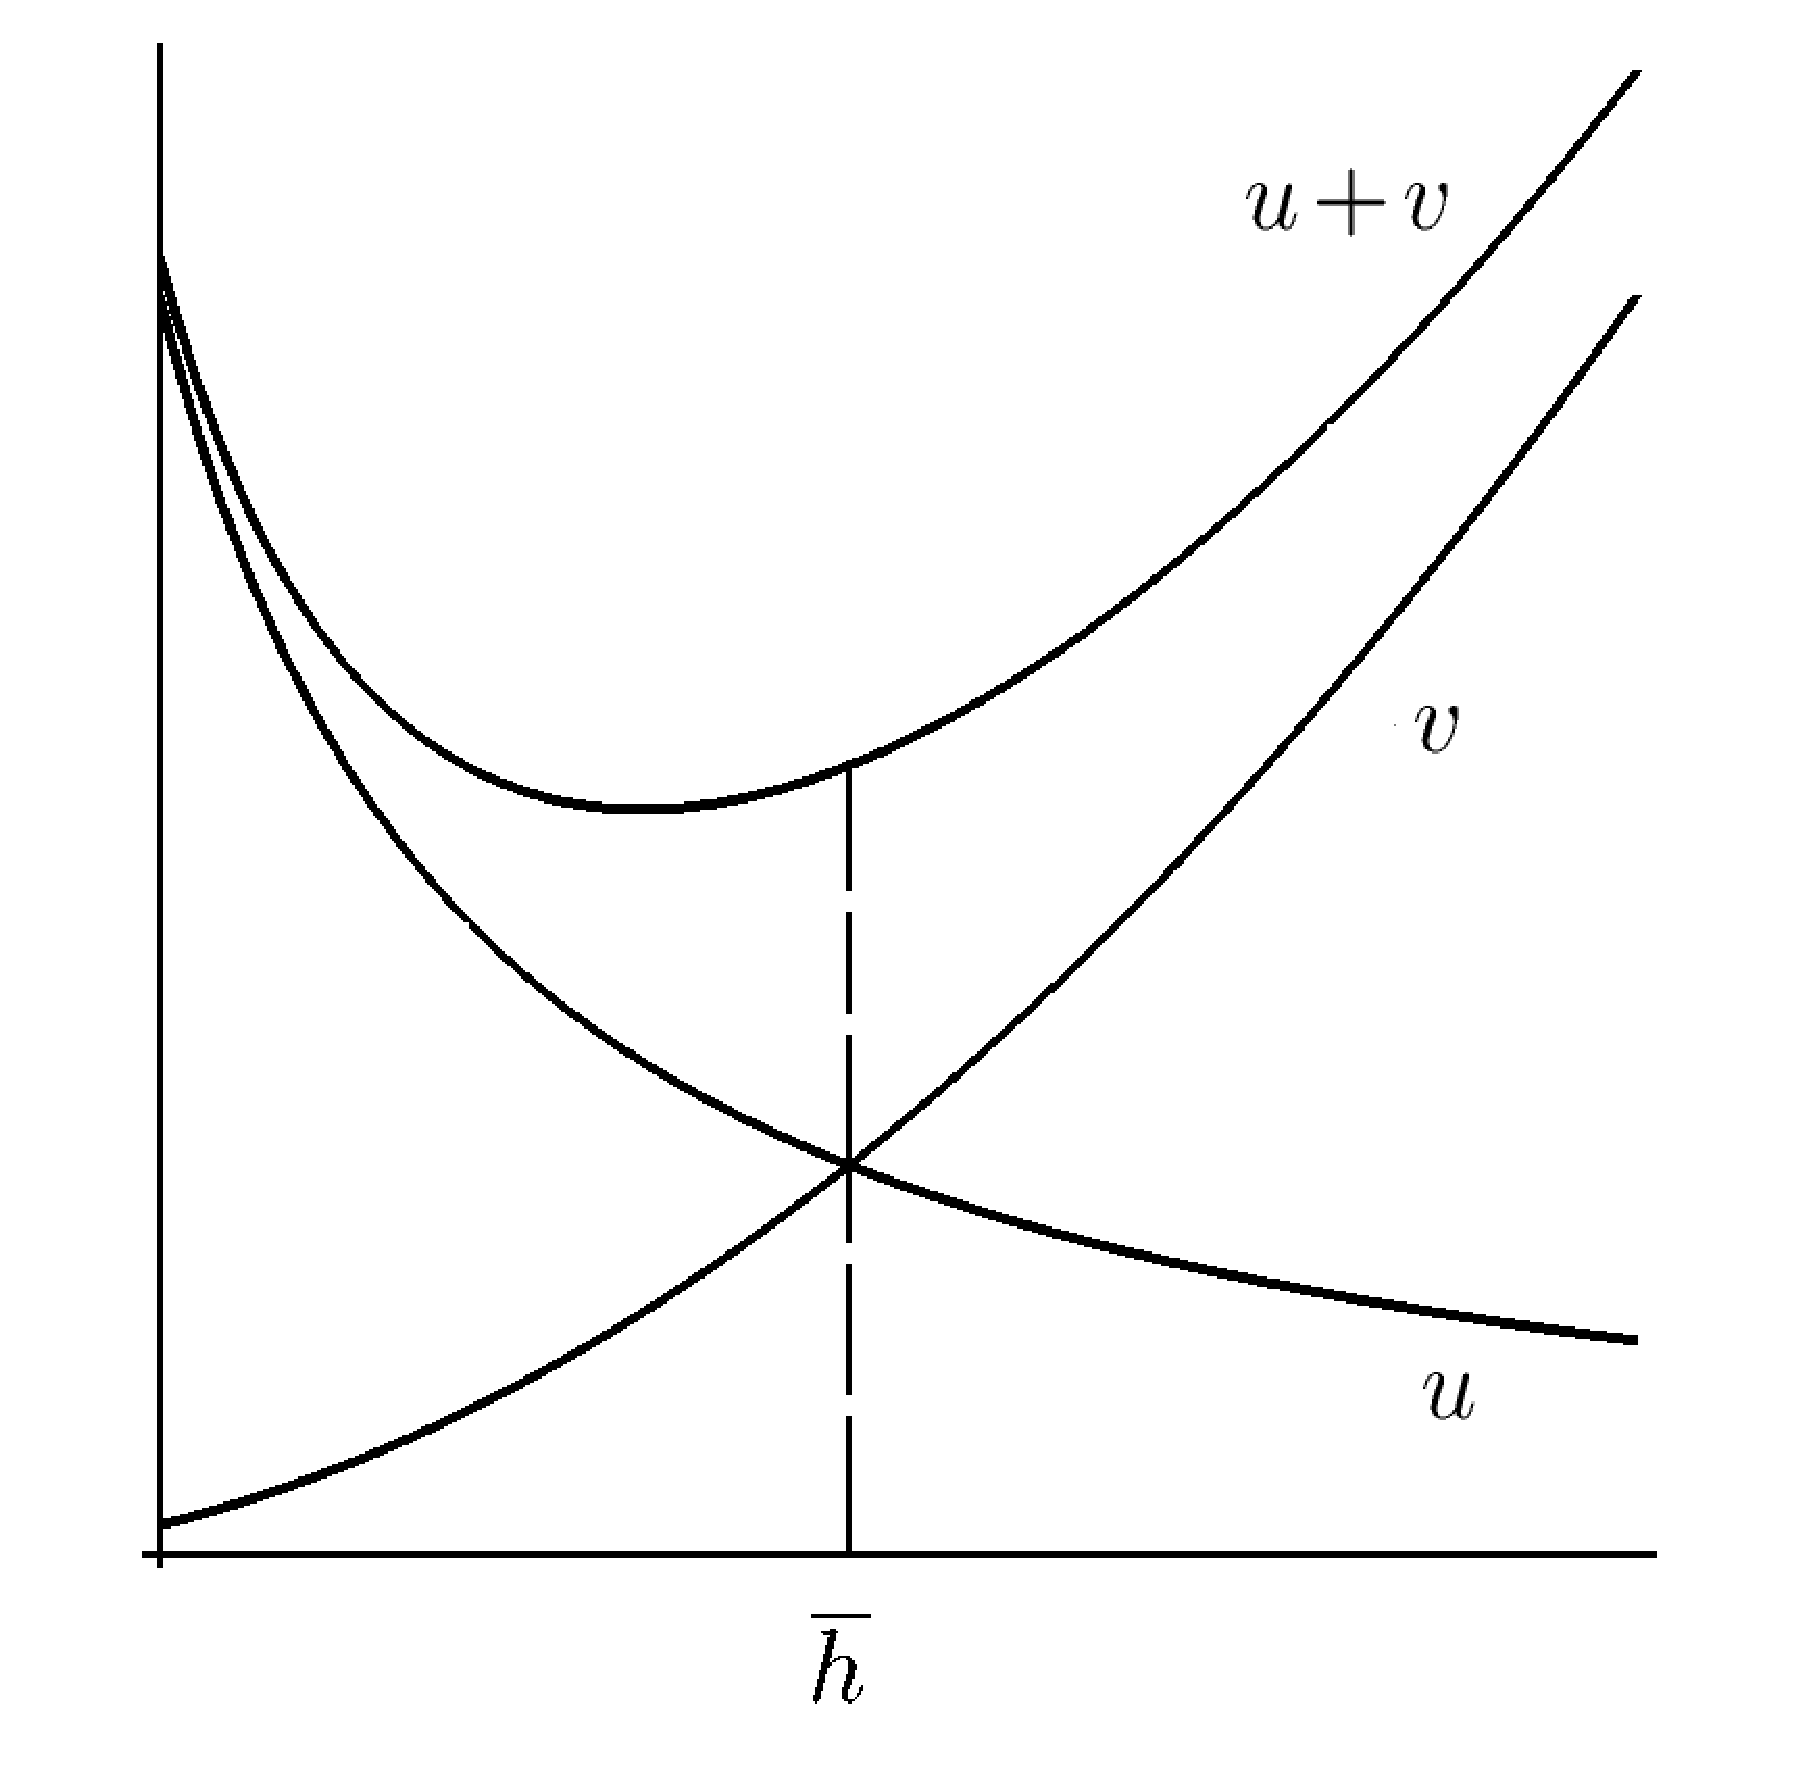
\includegraphics[width=0.4\textwidth]{pict/pict20-1.eps}
\end{center}
 \bigskip
 \refstepcounter{ris}\label{r20-1}

 \centerline{╨а╨╕╤Б.~\theris}
 \bigskip
\end{figure}


╨Т ╨┐╤А╨░╨▓╨╛╨╣ ╤З╨░╤Б╤В╨╕~(\ref{f20-4}) ╤Б╨╗╨░╨│╨░╨╡╨╝╨╛╨╡  $h^{-k}$ ╤Г╨▒╤Л╨▓╨░╨╡╤В, ╨░ $h^{l-k}$
╨▓╨╛╨╖╤А╨░╤Б╤В╨░╨╡╤В; ╨╕╤Б╤Е╨╛╨┤╤П ╨╕╨╖ ╤Б╤Д╨╛╤А╨╝╤Г╨╗╨╕╤А╨╛╨▓╨░╨╜╨╜╨╛╨│╨╛ ╨┐╤А╨╕╨╜╤Ж╨╕╨┐╨░ ╨▓╤Л╨▒╨╡╤А╨╡╨╝ ╤В╨╛╤З╨║╤Г
 $h=\overline h$ ╨╕╨╖
 ╤Г╤Б╨╗╨╛╨▓╨╕╤П $(\overline h)^{-k}\|f\|_C=(\overline h)^{l-k}\|f^{(l)}\|_C,$ ╤З╤В╨╛ ╨┤╨░╨╡╤В ╨╖╨╜╨░╤З╨╡╨╜╨╕╨╡
 $$
  \overline h=\left( \frac{\|f\|_C}{\|f^{(l)}\|_C}\right)^{\frac{1}{l}}.
 $$
 ╨Я╨╛╨┤╤Б╤В╨░╨▓╨╕╨▓ ╨╜╨░╨╣╨┤╨╡╨╜╨╜╨╛╨╡ ╨╖╨╜╨░╤З╨╡╨╜╨╕╨╡ $h$
 ╨▓~(\ref{f20-4}), ╨┐╨╛╨╗╤Г╤З╨╕╨╝ ╨╜╨╡╤А╨░╨▓╨╡╨╜╤Б╤В╨▓╨╛ ╨Ъ╨╛╨╗╨╝╨╛╨│╨╛╤А╨╛╨▓╨░
 $$
 \|f^{(k)}\|_C\le {2C_k}\|f\|_C^{\frac{l-k}{l}}\|f^{(l)}\|_C^{\frac{k}{l}}.
 $$
 ╨в╨╡╨╛╤А╨╡╨╝╨░ ╨┤╨╛╨║╨░╨╖╨░╨╜╨░ ╤Б ╨║╨╛╨╜╤Б╤В╨░╨╜╤В╨╛╨╣, ╨╜╨╡ ╨╖╨░╨▓╨╕╤Б╤П╤Й╨╡╨╣ ╨╛╤В $n:\ K_{n,k}\le \pi A_k.$

 ╨Ч\,╨░\,╨╝\,╨╡\,╤З\,╨░\,╨╜\,╨╕\,╤П.\quad
 1) ╨Э╨╡╤А╨░╨▓╨╡╨╜╤Б╤В╨▓╨╛ ╨Ъ╨╛╨╗╨╝╨╛╨│╨╛╤А╨╛╨▓╨░ ╨▓╨╡╤А╨╜╨╛   ╨╕ ╨┤╨╛╨║╨░╨╖╨░╤В╨╡╨╗╤М╤Б╤В╨▓╨╛ ╨┐╤А╨╛╤Е╨╛╨┤╨╕╤В
 ╨┤╨╗╤П ╨╗╤О╨▒╨╛╨│╨╛ ╨╛╨┤╨╜╨╛╤А╨╛╨┤╨╜╨╛╨│╨╛ ╨┐╤А╨╛╤Б╤В╤А╨░╨╜╤Б╤В╨▓╨░
 $2\pi$-╨┐╨╡╤А╨╕╨╛╨┤╨╕╤З╨╡╤Б╨║╨╕╤Е ╤Д╤Г╨╜╨║╤Ж╨╕╨╣ (╤Б╨╝. ╨╖╨░╨╝╨╡╤З╨░╨╜╨╕╨╡~\ref{r16-1}), ╤В╨░╨║ ╨║╨░╨║
 ╨╛╨▒╨╛╨▒╤Й╨╡╨╜╨╜╨╛╨╡ ╨╜╨╡╤А╨░╨▓╨╡╨╜╤Б╤В╨▓╨╛ ╨С╨╡╤А╨╜╤И╤В╨╡╨╣╨╜╨░ ╨▓╨╡╤А╨╜╨╛ ╨┤╨╗╤П ╤Н╤В╨╕╤Е
 ╨┐╤А╨╛╤Б╤В╤А╨░╨╜╤Б╤В╨▓. ╨Т ╤З╨░╤Б╤В╨╜╨╛╤Б╤В╨╕, ╨╛╨╜╨╛ ╤Б╨┐╤А╨░╨▓╨╡╨┤╨╗╨╕╨▓╨╛ ╨▓ $L_{2\pi}^p$

 2) ╨Ъ╨░╨║ ╤Г╨╢╨╡ ╨╛╤В╨╝╨╡╤З╨░╨╗╨╛╤Б╤М ╨▓ ╨╗╨╡╨║╤Ж╨╕╨╕ 19, ╨╜╨╡╤А╨░╨▓╨╡╨╜╤Б╤В╨▓╨╛~(\ref{f20-1}) ╤Б╨┐╤А╨░╨▓╨╡╨┤╨╗╨╕╨▓╨╛ ╨╕ ╨┤╨╗╤П ╤Д╤Г╨╜╨║╤Ж╨╕╨╣ ╨╜╨░ ╨▓╤Б╨╡╨╣
 ╤З╨╕╤Б╨╗╨╛╨▓╨╛╨╣ ╨┐╤А╤П╨╝╨╛╨╣.


 ╨б╨╝╤Л╤Б╨╗ ╨╜╨╡╤А╨░╨▓╨╡╨╜╤Б╤В╨▓╨░ ╨Ъ╨╛╨╗╨╝╨╛╨│╨╛╤А╨╛╨▓╨░ ╨╖╨░╨║╨╗╤О╤З╨░╨╡╤В╤Б╤П ╨▓
 ╤Б╨╗╨╡╨┤╤Г╤О╤Й╨╡╨╝: ╨╡╤Б╨╗╨╕ ╨║╨░╨║╨╛╨╝╤Г-╤В╨╛ ╨┐╤А╨╛╤Б╤В╤А╨░╨╜╤Б╤В╨▓╤Г ╨┐╤А╨╕╨╜╨░╨┤╨╗╨╡╨╢╨╕╤В
 ╤Д╤Г╨╜╨║╤Ж╨╕╤П ╨╕ ╨╡╨╡ ╤Б╤В╨░╤А╤И╨░╤П ╨┐╤А╨╛╨╕╨╖╨▓╨╛╨┤╨╜╨░╤П $f^{(l)},$
 ╤В╨╛ ╤В╨╛╨╝╤Г ╨╢╨╡ ╨┐╤А╨╛╤Б╤В╤А╨░╨╜╤Б╤В╨▓╤Г ╨┐╤А╨╕╨╜╨░╨┤╨╗╨╡╨╢╨░╤В ╨╕ ╨▓╤Б╨╡ ╨┐╤А╨╛╨╝╨╡╨╢╤Г╤В╨╛╤З╨╜╤Л╨╡
 ╨┐╤А╨╛╨╕╨╖╨▓╨╛╨┤╨╜╤Л╨╡.

 ╨Э╨╡╤А╨░╨▓╨╡╨╜╤Б╤В╨▓╨╛ ╨Ъ╨╛╨╗╨╝╨╛╨│╨╛╤А╨╛╨▓╨░ ╨╡╤Б╤В╤М ╤А╨╡╤И╨╡╨╜╨╕╨╡ ╤Б╨╗╨╡╨┤╤Г╤О╤Й╨╡╨╣
  ╨╖╨░╨┤╨░╤З╨╕. ╨Я╤Г╤Б╤В╤М  ╨╖╨░╨┤╨░╨╜╤Л ╤З╨╕╤Б╨╗╨░ $M_l\ge 0$ ╨╕ $M_0\ge 0.$
 ╨а╨░╤Б╤Б╨╝╨╛╤В╤А╨╕╨╝ ╨▓╤Б╨╡ $l$ ╤А╨░╨╖ ╨┤╨╕╤Д╤Д╨╡╤А╨╡╨╜╤Ж╨╕╤А╤Г╨╡╨╝╤Л╨╡ ╤Д╤Г╨╜╨║╤Ж╨╕╨╕ $f,$
  ╤Г ╨║╨╛╤В╨╛╤А╤Л╤Е
 $$
 \|f\|_C=M_0,\qquad \|f^{(l)}\|_C=M_l.
 $$
 ╨Ъ╨░╨║╨╛╨▓╨░ ╤В╨╛╨│╨┤╨░ ╨╛╨▒╨╗╨░╤Б╤В╤М ╨╕╨╖╨╝╨╡╨╜╨╡╨╜╨╕╤П ╨╜╨╛╤А╨╝ $\|f^{(k)}\|_C$
 ╨╕, ╨▓ ╤З╨░╤Б╤В╨╜╨╛╤Б╤В╨╕,  ╤З╨╡╨╝╤Г ╤А╨░╨▓╨╜╨╛ $M_k=\max\|f^{(k)}\|_C?$
 ╨н╤В╨░ ╨╛╨▒╨╗╨░╤Б╤В╤М ╨╛╨┐╨╕╤Б╤Л╨▓╨░╨╡╤В╤Б╤П ╨╜╨╡╤А╨░╨▓╨╡╨╜╤Б╤В╨▓╨╛╨╝ ╨Ъ╨╛╨╗╨╝╨╛╨│╨╛╤А╨╛╨▓╨░.

 \section{╨в╨╡╨╛╤А╨╡╨╝╨░ ╨╛ ╨┐╨╛╤З╨╗╨╡╨╜╨╜╨╛╨╝ ╨┤╨╕╤Д╤Д╨╡╤А╨╡╨╜╤Ж╨╕╤А╨╛╨▓╨░╨╜╨╕╨╕\\ ╤Д╤Г╨╜╨║╤Ж╨╕╨╛╨╜╨░╨╗╤М╨╜╤Л╤Е
 ╨┐╨╛╤Б╨╗╨╡╨┤╨╛╨▓╨░╤В╨╡╨╗╤М╨╜╨╛╤Б╤В╨╡╨╣}

 ╨а╨░╤Б╤Б╨╝╨╛╤В╤А╨╕╨╝ ╨╖╨░╨┤╨░╤З╤Г. ╨Я╤Г╤Б╤В╤М ╨┤╨░╨╜╨░ ╨┐╨╛╤Б╨╗╨╡╨┤╨╛╨▓╨░╤В╨╡╨╗╤М╨╜╨╛╤Б╤В╤М ╨┐╨╡╤А╨╕╨╛╨┤╨╕╤З╨╡╤Б╨║╨╕╤Е
 ╤Д╤Г╨╜╨║╤Ж╨╕╨╣ $\{f_n\}$ ╤А╨░╨▓╨╜╨╛╨╝╨╡╤А╨╜╨╛ ╤Б╤Е╨╛╨┤╤П╤Й╨░╤П╤Б╤П ╨║ ╤Д╤Г╨╜╨║╤Ж╨╕╨╕ $f$:~ $f_n\rightrightarrows
 f$ ╨╕ ╤Д╤Г╨╜╨║╤Ж╨╕╨╕ $f_n$ ╨╕╨╝╨╡╤О╤В $k$-╤Г╤О ╨┐╤А╨╛╨╕╨╖╨▓╨╛╨┤╨╜╤Г╤О.
 ╨Я╤А╨╕ ╨║╨░╨║╨╕╤Е ╤Г╤Б╨╗╨╛╨▓╨╕╤П╤Е ╨┐╤А╨╡╨┤╨╡╨╗╤М╨╜╨░╤П ╤Д╤Г╨╜╨║╤Ж╨╕╤П ╨┤╨╕╤Д╤Д╨╡╤А╨╡╨╜╤Ж╨╕╤А╤Г╨╡╨╝╨░ $k$
 ╤А╨░╨╖ ╨╕ $f_n^{(k)} \rightrightarrows f^{(k)}?$

╨Я╤А╨╡╨┤╨┐╨╛╨╗╨╛╨╢╨╕╨╝, ╨╕╨╖╨▓╨╡╤Б╤В╨╜╨╛, ╤З╤В╨╛ ╨┐╤А╨╛╨╕╨╖╨▓╨╛╨┤╨╜╤Л╨╡ ╨╜╨╡╨║╨╛╤В╨╛╤А╨╛╨│╨╛ ╨┐╨╛╤А╤П╨┤╨║╨░  $l>k$ ╤З╨╗╨╡╨╜╨╛╨▓
╨┐╨╛╤Б╨╗╨╡╨┤╨╛╨▓╨░╤В╨╡╨╗╤М╨╜╨╛╤Б╤В╨╕ ╤Б╤Г╤Й╨╡╤Б╤В╨▓╤Г╤О╤В ╨╕ ╨╛╨│╤А╨░╨╜╨╕╤З╨╡╨╜╤Л ╨╜╨╡╨║╨╛╤В╨╛╤А╨╛╨╣ ╨║╨╛╨╜╤Б╤В╨░╨╜╤В╨╛╨╣:
 $\|f_n^{(l)}\|_C\le {A},\ n\ge 1.$
 ╨Э╨░╨┐╨╕╤И╨╡╨╝ ╨╜╨╡╤А╨░╨▓╨╡╨╜╤Б╤В╨▓╨╛ ╨Ъ╨╛╨╗╨╝╨╛╨│╨╛╤А╨╛╨▓╨░ ╨┤╨╗╤П ╤А╨░╨╖╨╜╨╛╤Б╤В╨╡╨╣ $f_n-f_m$:
  $$
 \|f_n^{(k)}-f_m^{(k)}\|_C\le K \|f_n-f_m\|_C^{\frac{k}{l}}\cdot
 (2{A})^{\frac{l-k}{l}};
 $$
 ╨┐╨╛╤Б╨╗╨╡╨┤╨╜╨╡╨╡ ╨╜╨╡╤А╨░╨▓╨╡╨╜╤Б╤В╨▓╨╛ ╨┐╨╛╨║╨░╨╖╤Л╨▓╨░╨╡╤В, ╤З╤В╨╛ ╨┐╨╛╤Б╨╗╨╡╨┤╨╛╨▓╨░╤В╨╡╨╗╤М╨╜╨╛╤Б╤В╤М ╨┐╤А╨╛╨╕╨╖╨▓╨╛╨┤╨╜╤Л╤Е $\{f_n^{(k)}\}$
 ╤П╨▓╨╗╤П╨╡╤В╤Б╤П ╤Д╤Г╨╜╨┤╨░╨╝╨╡╨╜╤В╨░╨╗╤М╨╜╨╛╨╣ (╨┐╨╛╤Б╨╗╨╡╨┤╨╛╨▓╨░╤В╨╡╨╗╤М╨╜╨╛╤Б╤В╤М╤О ╨Ъ╨╛╤И╨╕) ╨╕, ╨╖╨╜╨░╤З╨╕╤В,
 ╤А╨░╨▓╨╜╨╛╨╝╨╡╤А╨╜╨╛ ╤Б╤Е╨╛╨┤╨╕╤В╤Б╤П ╨║ ╨╜╨╡╨║╨╛╤В╨╛╤А╨╛╨╣ ╤Д╤Г╨╜╨║╤Ж╨╕╨╕ $\varphi.$
 ╨Э╨╛ ╤В╨╛╨│╨┤╨░ ╨▓ ╤Б╨╕╨╗╤Г ╤Б╨╛╨╛╤В╨▓╨╡╤В╤Б╤В╨▓╤Г╤О╤Й╨╡╨╣ ╤В╨╡╨╛╤А╨╡╨╝╤Л ╨╛ ╤А╨░╨▓╨╜╨╛╨╝╨╡╤А╨╜╨╛ ╤Б╤Е╨╛╨┤╤П╤Й╨╕╤Е╤Б╤П
 ╨┐╨╛╤Б╨╗╨╡╨┤╨╛╨▓╨░╤В╨╡╨╗╤М╨╜╨╛╤Б╤В╤П╤Е ╨┤╨╕╤Д╤Д╨╡╤А╨╡╨╜╤Ж╨╕╤А╤Г╨╡╨╝╤Л╤Е ╤Д╤Г╨╜╨║╤Ж╨╕╨╣ ╨╝╨╛╨╢╨╜╨╛ ╤Г╤В╨▓╨╡╤А╨╢╨┤╨░╤В╤М,
 ╤З╤В╨╛ ╤Д╤Г╨╜╨║╤Ж╨╕╤П $f$ ╤П╨▓╨╗╤П╨╡╤В╤Б╤П $k$ ╤А╨░╨╖ ╨┤╨╕╤Д╤Д╨╡╤А╨╡╨╜╤Ж╨╕╤А╤Г╨╡╨╝╨╛╨╣ ╨╕ $\varphi=f^{(k)}$.

 ╨Ю╤В╤Б╤О╨┤╨░ ╤Б╨╗╨╡╨┤╤Г╨╡╤В, ╤З╤В╨╛ ╨╜╨░ ╨║╨╗╨░╤Б╤Б╨╡  ╤Д╤Г╨╜╨║╤Ж╨╕╨╣, $l$
 ╤А╨░╨╖ ╨┤╨╕╤Д╤Д╨╡╤А╨╡╨╜╤Ж╨╕╤А╤Г╨╡╨╝╤Л╤Е, ╤Б ╨┐╤А╨╛╨╕╨╖╨▓╨╛╨┤╨╜╨╛╨╣ ╨┐╨╛╤А╤П╨┤╨║╨░ $l,$ ╨╛╨│╤А╨░╨╜╨╕╤З╨╡╨╜╨╜╨╛╨╣ ╨╜╨╡╨║╨╛╤В╨╛╤А╨╛╨╣ ╨║╨╛╨╜╤Б╤В╨░╨╜╤В╨╛╨╣,
 ╨╛╨┐╨╡╤А╨░╤Ж╨╕╤П ╨┤╨╕╤Д╤Д╨╡╤А╨╡╨╜╤Ж╨╕╤А╨╛╨▓╨░╨╜╨╕╤П ╨┐╨╛╤А╤П╨┤╨║╨░  $k,$~ $0<k<l,$ ╨║╨╛╤А╤А╨╡╨║╤В╨╜╨░, ╨░ ╤В╨╛╤З╨╜╨╡╨╡, ╨╛╨┐╨╡╤А╨░╤В╨╛╤А
 ╨┤╨╕╤Д╤Д╨╡╤А╨╡╨╜╤Ж╨╕╤А╨╛╨▓╨░╨╜╨╕╤П ╨┐╨╛╤А╤П╨┤╨║╨░ $k$ ╨╜╨╡╨┐╤А╨╡╤А╤Л╨▓╨╡╨╜. ╨н╤В╨╛
 ╨╛╨╖╨╜╨░╤З╨░╨╡╤В, ╤З╤В╨╛ ╨╜╨░ ╤В╨░╨║╨╛╨╝ ╨║╨╗╨░╤Б╤Б╨╡ ╨╕╨╝╨╡╨╡╤В ╨╝╨╡╤Б╤В╨╛ ╤А╨╡╨│╤Г╨╗╤П╤А╨╕╨╖╨░╤Ж╨╕╤П ╨╛╨┐╨╡╤А╨░╤В╨╛╤А╨░
 ╨┤╨╕╤Д╤Д╨╡╤А╨╡╨╜╤Ж╨╕╤А╨╛╨▓╨░╨╜╨╕╤П: ╨╝╨░╨╗╨░╤П ╨╛╤И╨╕╨▒╨║╨░ ╨▓ ╨╛╨┐╤А╨╡╨┤╨╡╨╗╨╡╨╜╨╕╨╕ ╤Д╤Г╨╜╨║╤Ж╨╕╨╕ $f$
 ╨╕╨╖ ╨║╨╗╨░╤Б╤Б╨░ ╨│╨░╤А╨░╨╜╤В╨╕╤А╤Г╨╡╤В ╨╝╨░╨╗╨╛╤Б╤В╤М ╨╛╤И╨╕╨▒╨║╨╕ ╨▓╤Л╤З╨╕╤Б╨╗╨╡╨╜╨╕╤П
 ╨┐╤А╨╛╨╕╨╖╨▓╨╛╨┤╨╜╤Л╤Е $f^{(k)}\ (0<k<l)$ ╨┐╤А╨╕ ╨┐╨╛╨┤╤Е╨╛╨┤╤П╤Й╨╡╨╝ ╨╝╨╡╤В╨╛╨┤╨╡ ╨╕╤Е
 ╨▓╨╛╤Б╤Б╤В╨░╨╜╨╛╨▓╨╗╨╡╨╜╨╕╤П ╨┐╨╛ $\widetilde{f}(x) (\approx f(x)).$

 ╨Я╤Г╤Б╤В╤М $f\in {C}^{(l)}_{{2\pi}}$ ╨╕ $t_n$~--
 ╨╜╨╡╨║╨╛╤В╨╛╤А╤Л╨╣ ╤В╤А╨╕╨│╨╛╨╜╨╛╨╝╨╡╤В╤А╨╕╤З╨╡╤Б╨║╨╕╨╣ ╨┐╨╛╨╗╨╕╨╜╨╛╨╝.
 ╨Я╤А╨╕╨╝╨╡╨╜╨╕╨╝ ╨║ ╤А╨░╨╖╨╜╨╛╤Б╤В╨╕ $f-t_n$ ╨╜╨╡╤А╨░╨▓╨╡╨╜╤Б╤В╨▓╨╛ ╨Ъ╨╛╨╗╨╝╨╛╨│╨╛╤А╨╛╨▓╨░:
 $$
 \|f^{(k)}-t_n^{(k)}\|_C\le K \|f-t_n\|_C^{\frac{k}{{l}}}\cdot
 \|f^{(l)}-t_n^{(l)}\|_C^{\frac{l-k}{l}}.
 $$
 ╨Ю╤В╤Б╤О╨┤╨░ ╤Б╨╗╨╡╨┤╤Г╨╡╤В, ╤З╤В╨╛ ╨╡╤Б╨╗╨╕ ╤Д╤Г╨╜╨║╤Ж╨╕╤П ╨╕  ╨╡╨╡ ╤Б╤В╨░╤А╤И╨░╤П ╨┐╤А╨╛╨╕╨╖╨▓╨╛╨┤╨╜╨░╤П
 ╤Е╨╛╤А╨╛╤И╨╛ ╨┐╤А╨╕╨▒╨╗╨╕╨╢╨░╤О╤В╤Б╤П ╤В╤А╨╕╨│╨╛╨╜╨╛╨╝╨╡╤В╤А╨╕╤З╨╡╤Б╨║╨╕╨╝ ╨┐╨╛╨╗╨╕╨╜╨╛╨╝╨╛╨╝ ╨╕ ╨╡╨│╨╛
 {╤Б╤В╨░╤А╤И╨╡╨╣} ╨┐╤А╨╛╨╕╨╖╨▓╨╛╨┤╨╜╨╛╨╣, ╤В╨╛ ╨╕ ╨┐╤А╨╛╨╝╨╡╨╢╤Г╤В╨╛╤З╨╜╤Л╨╡ ╨┐╤А╨╛╨╕╨╖╨▓╨╛╨┤╨╜╤Л╨╡
 ╤Д╤Г╨╜╨║╤Ж╨╕╨╕ ╤В╨╛╨╢╨╡ ╤Е╨╛╤А╨╛╤И╨╛ ╨┐╤А╨╕╨▒╨╗╨╕╨╢╨░╤О╤В╤Б╤П
 {╤Б╨╛╨╛╤В╨▓╨╡╤В╤Б╤В╨▓╤Г╤О╤Й╨╕╨╝╨╕} {╨┐╤А╨╛╨╕╨╖╨▓╨╛╨┤╨╜╤Л╨╝╨╕ ╨┐╨╛╨╗╨╕╨╜╨╛╨╝╨░}.

 ╨Х╤Б╨╗╨╕ ╨▓ ╨║╨░╤З╨╡╤Б╤В╨▓╨╡ $t_n$ ╨▓╨╛╨╖╤М╨╝╨╡╨╝ ╤Б╤Г╨╝╨╝╤Л ╨д╤Г╤А╤М╨╡, ╤В╨╛ ╨┐╨╛╨╗╤Г╤З╨╕╨╝ ╨╛╤Ж╨╡╨╜╨║╤Г
 $$
   \|f^{(k)}-s_n^{(k)}\|_C\le K_{{1}} \|f-s_n \|_C^{\frac{k}{l}}\cdot
   \Big(\ln (n+1)  {E_n(f^{(l)})\Big)^{\frac{l-k}{l}},\qquad n\ge 1},
 $$
 ╨║╨╛╤В╨╛╤А╨░╤П ╨┤╨░╨╡╤В ╤Б╨▓╤П╨╖╤М ╨╝╨╡╨╢╨┤╤Г ╨┐╤А╨╕╨▒╨╗╨╕╨╢╨╡╨╜╨╕╤П╨╝╨╕ ╨┐╤А╨╛╨╕╨╖╨▓╨╛╨┤╨╜╨╛╨╣ ╨╕ ╤Д╤Г╨╜╨║╤Ж╨╕╨╕
 ╤Б╤Г╨╝╨╝╨░╨╝╨╕ ╨д╤Г╤А╤М╨╡.

 ╨Ю╤В╨╝╨╡╤В╨╕╨╝, ╤З╤В╨╛ ╨▓ ╨╜╨╡╤А╨░╨▓╨╡╨╜╤Б╤В╨▓╨╡ ╨Ъ╨╛╨╗╨╝╨╛╨│╨╛╤А╨╛╨▓╨░~(\ref{f20-1}) ╨▓ ╨┐╤А╨╛╤Б╤В╤А╨░╨╜╤Б╤В╨▓╨╡ $C_{2\pi}$
 ╨╜╨╡╨╗╤М╨╖╤П ╨╖╨░╨╝╨╡╨╜╨╕╤В╤М ╨╜╨╛╤А╨╝╤Л ╨╜╨░ ╨╜╨░╨╕╨╗╤Г╤З╤И╨╕╨╡ ╨┐╤А╨╕╨▒╨╗╨╕╨╢╨╡╨╜╨╕╤П, ╤В╨░╨║ ╨║╨░╨║ ╨▓
 ╨┐╤А╨╛╤Б╤В╤А╨░╨╜╤Б╤В╨▓╨╡ $C_{2\pi}$ ╨╜╨░╨╕╨╗╤Г╤З╤И╨╕╨╣ ╨┐╨╛╨╗╨╕╨╜╨╛╨╝ ╨┤╨╗╤П ╨┐╤А╨╛╨╕╨╖╨▓╨╛╨┤╨╜╨╛╨╣ ╨╝╨╛╨╢╨╡╤В ╨╜╨╡ ╨▒╤Л╤В╤М
 ╨┐╤А╨╛╨╕╨╖╨▓╨╛╨┤╨╜╨╛╨╣ ╨╛╤В ╨╜╨░╨╕╨╗╤Г╤З╤И╨╡╨│╨╛ ╨┐╨╛╨╗╨╕╨╜╨╛╨╝╨░ ╨┤╨╗╤П ╤Д╤Г╨╜╨║╤Ж╨╕╨╕. ╨Т $L_2$ ╤В╨░╨║╨░╤П ╨╖╨░╨╝╨╡╨╜╨░ ╨▓╨╛╨╖╨╝╨╛╨╢╨╜╨░.

╨Ш╨╝╨╡╨╡╤В╤Б╤П ╨▒╨╛╨╗╤М╤И╨╛╨╡ ╤З╨╕╤Б╨╗╨╛ ╨╕╤Б╤Б╨╗╨╡╨┤╨╛╨▓╨░╨╜╨╕╨╣, ╨┐╨╛╤Б╨▓╤П╤Й╨╡╨╜╨╜╤Л╤Е ╨▒╨╛╨╗╨╡╨╡ ╨╛╨▒╤Й╨╕╨╝
 ╨▓ ╤Б╤А╨░╨▓╨╜╨╡╨╜╨╕╨╕ ╤Б~(\ref{f20-1}) ╨╜╨╡╤А╨░╨▓╨╡╨╜╤Б╤В╨▓╨░╨╝\footnote{╨Ш╨╜╤Д╨╛╤А╨╝╨░╤Ж╨╕╤О ╨┐╨╛
 ╤Н╤В╨╛╨╣ ╤В╨╡╨╝╨░╤В╨╕╨║╨╡ ╨╝╨╛╨╢╨╜╨╛ ╨╜╨░╨╣╤В╨╕ ╨▓ ╨╛╨▒╨╖╨╛╤А╨╜╨╛╨╣ ╤А╨░╨▒╨╛╤В╨╡:
╨Р╤А╨╡╤Б╤В╨╛╨▓ ╨Т.\,╨Т. ╨Я╤А╨╕╨▒╨╗╨╕╨╢╨╡╨╜╨╕╨╡ ╨╜╨╡╨╛╨│╤А╨░╨╜╨╕╤З╨╡╨╜╨╜╤Л╤Е ╨╛╨┐╨╡╤А╨░╤В╨╛╤А╨╛╨▓ ╨╛╨│╤А╨░╨╜╨╕╤З╨╡╨╜╨╜╤Л╨╝╨╕ ╨╕
╤А╨╛╨┤╤Б╤В╨▓╨╡╨╜╨╜╤Л╨╡ ╤Н╨║╤Б╤В╤А╨╡╨╝╨░╨╗╤М╨╜╤Л╨╡ ╨╖╨░╨┤╨░╤З╨╕
 // ╨г╤Б╨┐╨╡╤Е╨╕ ╨╝╨░╤В╨╡╨╝. ╨╜╨░╤Г╨║. 1996. ╨в.\,51, ╨▓╤Л╨┐.\,6. ╨б.\,89--124.}
 $$
 \|f^{(k)}\|_{L_q}\le K\|f\|_{L_p}^{\alpha}\cdot
 \|f^{(l)}\|_{L_r}^{\beta}.
 $$


 \section{╨Э╨╡╤А╨░╨▓╨╡╨╜╤Б╤В╨▓╨╛ ╨Ф╨╢╨╡╨║╤Б╨╛╨╜╨░}

 {╨Я╤А╨╛╨╝╨╡╨╢╤Г╤В╨╛╤З╨╜╤Л╨╡ ╨┐╤А╨╕╨▒╨╗╨╕╨╢╨╡╨╜╨╕╤П (╨┐╤А╨╕╨▒╨╗╨╕╨╢╨╡╨╜╨╕╤П ╨│╨╗╨░╨┤╨║╨╕╨╝╨╕
 ╤Д╤Г╨╜╨║╤Ж╨╕╤П╨╝╨╕)}
 \vspace{3mm}

 ╨Ш╨╖╨▓╨╡╤Б╤В╨╜╨╛, ╤З╤В╨╛ ╨▓╤Б╤П╨║╤Г╤О ╨╜╨╡╨┐╤А╨╡╤А╤Л╨▓╨╜╤Г╤О ╨┐╨╡╤А╨╕╨╛╨┤╨╕╤З╨╡╤Б╨║╤Г╤О  ╤Д╤Г╨╜╨║╤Ж╨╕╤О ╨╝╨╛╨╢╨╜╨╛ ╤Б╨║╨╛╨╗╤М╨║╨╛ ╤Г╨│╨╛╨┤╨╜╨╛
 ╤В╨╛╤З╨╜╨╛ ╨┐╤А╨╕╨▒╨╗╨╕╨╖╨╕╤В╤М ╨│╨╗╨░╨┤╨║╨╕╨╝╨╕ ╤Д╤Г╨╜╨║╤Ж╨╕╤П╨╝╨╕. ╨Э╨░╨┐╤А╨╕╨╝╨╡╤А, ╤Б╤Г╨╝╨╝╨░╨╝╨╕
 ╨д╨╡╨╣╨╡╤А╨░:
 $$
 \forall\ f\in C_{{2\pi}}\qquad \forall\ \varepsilon>0\qquad \exists\ n:\qquad
 \|f-\sigma_n{(f)}\|_C<\varepsilon.
 $$
 ╨Ч╨░╨┤╨░╨┤╨╕╨╝ ╨╜╨╛╤А╨╝╨╕╤А╨╛╨▓╨╛╤З╨╜╤Л╨╡ ╨┐╨░╤А╨░╨╝╨╡╤В╤А╤Л. ╨Я╤Г╤Б╤В╤М $l$
 -- ╨╜╨░╤В╤Г╤А╨░╨╗╤М╨╜╨╛╨╡ ╤З╨╕╤Б╨╗╨╛ ╨╕ $M>0.$ ╨а╨░╤Б╤Б╨╝╨╛╤В╤А╨╕╨╝ ╨║╨╗╨░╤Б╤Б $C^{(l)}(M)$ ╨▓╤Б╨╡╤Е
 $l$ ╤А╨░╨╖ ╨╜╨╡╨┐╤А╨╡╤А╤Л╨▓╨╜╨╛ ╨┤╨╕╤Д╤Д╨╡╤А╨╡╨╜╤Ж╨╕╤А╤Г╨╡╨╝╤Л╤Е $2\pi$-╨┐╨╡╤А╨╕╨╛╨┤╨╕╤З╨╡╤Б╨║╨╕╤Е
 ╤Д╤Г╨╜╨║╤Ж╨╕╨╣ $\varphi,$ ╤Г ╨║╨╛╤В╨╛╤А╤Л╤Е  $\|\varphi^{(l)}\|_C\le M.$
 ╨Ъ╨╗╨░╤Б╤Б╨╛╨╝ $C^{(l)}(M)$ ($M$ -- ╤Д╨╕╨║╤Б╨╕╤А╨╛╨▓╨░╨╜╨╛) ╤Г╨╢╨╡ ╨╜╨╡╨╗╤М╨╖╤П  ╤Б╨║╨╛╨╗╤М ╤Г╨│╨╛╨┤╨╜╨╛ ╤В╨╛╤З╨╜╨╛
 ╨┐╤А╨╕╨▒╨╗╨╕╨╖╨╕╤В╤М ╨┐╤А╨╛╨╕╨╖╨▓╨╛╨╗╤М╨╜╤Г╤О
 ╤Д╤Г╨╜╨║╤Ж╨╕╤О. ╨Т╨╛╨╖╨╜╨╕╨║╨░╨╡╤В ╤Б╨╗╨╡╨┤╤Г╤О╤Й╨░╤П ╨┐╤А╨╛╨▒╨╗╨╡╨╝╨░.

 \task %%% ╨Ч╨░╨┤╨░╤З╨░.
 ╨Э╨░╨╣╤В╨╕
 $$
 \inf_{\varphi\in C^{(l)}(M)} \|f-\varphi\|_C=E(f,C^{(l)}(M)).
 $$
 ╨н╤В╨░ ╨╖╨░╨┤╨░╤З╨░ ╨▒╨╡╤Б╨║╨╛╨╜╨╡╤З╨╜╨╛╨╝╨╡╤А╨╜╨░╤П ╨╕ ╨╜╨╡╨╗╨╕╨╜╨╡╨╣╨╜╨░╤П.

\vspace{3mm}
 {\bf 1. ╨Ю ╤Б╨│╨╗╨░╨╢╨╕╨▓╨░╨╜╨╕╨╕ ╤Д╤Г╨╜╨║╤Ж╨╕╨╣}
 \vspace{3mm}

 ╨Я╤А╨╕ $l=1,2$ ╨║╨╗╨░╤Б╤Б╨╕╤З╨╡╤Б╨║╨╛╨╡ ╤А╨╡╤И╨╡╨╜╨╕╨╡ ╨╖╨░╨┤╨░╤З╨╕ ╨╛ ╤Б╨│╨╗╨░╨╢╨╕╨▓╨░╨╜╨╕╨╕ ╨┤╨░╨╡╤В╤Б╤П
 ╤Б ╨┐╨╛╨╝╨╛╤Й╤М╤О ╨╛╨┐╤А╨╡╨┤╨╡╨╗╤П╨╡╨╝╤Л╤Е ╨╜╨╕╨╢╨╡ ╤Д╤Г╨╜╨║╤Ж╨╕╨╣ ╨б╤В╨╡╨║╨╗╨╛╨▓╨░.

 ╨Я╤Г╤Б╤В╤М $h>0;$ ╤Г╤Б╤А╨╡╨┤╨╜╨╕╨╝ ╤Д╤Г╨╜╨║╤Ж╨╕╤О $f{\in C_{2\pi}}$ ╨┐╨╛ ╨╛╤В╤А╨╡╨╖╨║╤Г
 ╨┤╨╗╨╕╨╜╤Л $h$ ╤Б ╤Ж╨╡╨╜╤В╤А╨╛╨╝ ╨▓ ╤В╨╛╤З╨║╨╡ $x.$  ╨Т ╤А╨╡╨╖╤Г╨╗╤М╤В╨░╤В╨╡ ╨┐╨╛╨╗╤Г╤З╨╕╨╝ ╤Д╤Г╨╜╨║╤Ж╨╕╤О
    \begin{equation}\label{f20-VAS-1}
  f_h(x)=\frac{1}{h}
 \int_{-\frac{h}{2}}^{\frac{h}{2}} f(x+t)\, dt,
\end{equation}
 ╨║╨╛╤В╨╛╤А╨░╤П ╨╜╨░╨╖╤Л╨▓╨░╨╡╤В╤Б╤П  ╤Д╤Г╨╜╨║╤Ж╨╕╨╡╨╣ ╨б╤В╨╡╨║╨╗╨╛╨▓╨░. ╨б╨│╨╗╨░╨╢╨╡╨╜╨╜╨░╤П ╤Д╤Г╨╜╨║╤Ж╨╕╤П~(\ref{f20-VAS-1})
 ╤Г╨╢╨╡ ╨╜╨╡╨┐╤А╨╡╤А╤Л╨▓╨╜╨╛ ╨┤╨╕╤Д╤Д╨╡╤А╨╡╨╜╤Ж╨╕╤А╤Г╨╡╨╝╨░ ╨╕
 $$
 f_h'(x)=\frac{1}{h} \left\{ f\left( x+\frac{h}{2}\right)-f\left(
 x-\frac{h}{2}\right)\right\}.
 $$
 ╨б╨┐╤А╨░╨▓╨╡╨┤╨╗╨╕╨▓╤Л ╤Б╨╗╨╡╨┤╤Г╤О╤Й╨╕╨╡ ╤Б╨╛╨╛╤В╨╜╨╛╤И╨╡╨╜╨╕╤П:
 $$
 \|f_h'\|_C\le \frac{2}{h}\|f\|_C,
 $$
 $$
 \|f-f_h\|_C\le \frac{1}{h}
 \int_{-\frac{{h}}{2}}^{\frac{{h}}{2}} \| f(x)-f(x+t)\|_C\, dt\le
 \frac{2}{h}
 \int_{0}^{\frac{h}{2}} \omega(f,t)\, dt\le \omega\left(
 f,\frac{h}{2}\right).
 $$
 ╨б╨╗╨╡╨┤╨╛╨▓╨░╤В╨╡╨╗╤М╨╜╨╛, ╤Д╤Г╨╜╨║╤Ж╨╕╤П ╨б╤В╨╡╨║╨╗╨╛╨▓╨░ ╨┐╤А╨╕╨▒╨╗╨╕╨╢╨░╨╡╤В ╨╕╤Б╤Е╨╛╨┤╨╜╤Г╤О ╤Д╤Г╨╜╨║╤Ж╨╕╤О ╨╕ ╤П╨▓╨╗╤П╨╡╤В╤Б╤П ╨╜╨╡╨┐╤А╨╡╤А╤Л╨▓╨╜╨╛
 ╨┤╨╕╤Д╤Д╨╡╤А╨╡╨╜╤Ж╨╕╤А╤Г╨╡╨╝╨╛╨╣. ╨Ю╨┤╨╜╨░╨║╨╛, ╨┐╤А╨╕ ╤Е╨╛╤А╨╛╤И╨╡╨╝ ╨┐╤А╨╕╨▒╨╗╨╕╨╢╨╡╨╜╨╕╨╕ ╨┐╤А╨╛╨╕╨╖╨▓╨╛╨┤╨╜╨░╤П $f'_h,$ ╨▓╨╛╨╛╨▒╤Й╨╡ ╨│╨╛╨▓╨╛╤А╤П,
 ╨▒╤Г╨┤╨╡╤В ╨▒╨╛╨╗╤М╤И╨╛╨╣.

 ╨Я╨╛ ╨▓╨╡╤Й╨╡╤Б╤В╨▓╨╡╨╜╨╜╨╛╨╝╤Г ╤З╨╕╤Б╨╗╤Г $M>0$ ╨▓╤Л╨▒╨╡╤А╨╡╨╝ ╨┐╨░╤А╨░╨╝╨╡╤В╤А $h$ ╤В╨░╨║, ╤З╤В╨╛╨▒╤Л $M=\dfrac{2}{h}\|f\|_C,$
 ╤В.\,╨╡. ╨▓╨╛╨╖╤М╨╝╨╡╨╝ $h=\dfrac{2\|f\|_C}{M}.$ ╨Т ╤А╨╡╨╖╤Г╨╗╤М╤В╨░╤В╨╡ ╨┐╤А╨╕╤Е╨╛╨┤╨╕╨╝ ╨║ ╤Б╨╗╨╡╨┤╤Г╤О╤Й╨╡╨╝╤Г ╤Г╤В╨▓╨╡╤А╨╢╨┤╨╡╨╜╨╕╤О ╨╛ ╨┐╤А╨╕╨▒╨╗╨╕╨╢╨╡╨╜╨╕╨╕ ╤Д╤Г╨╜╨║╤Ж╨╕╤П╨╝╨╕ ╨б╤В╨╡╨║╨╗╨╛╨▓╨░.

 \begin{teo} ╨Ф╨╗╤П ╨║╨░╨╢╨┤╨╛╨╣ ╤Д╤Г╨╜╨║╤Ж╨╕╨╕ $f\in C_{{2\pi}}$ ╨╕ ╨╗╤О╨▒╨╛╨╣ ╨║╨╛╨╜╤Б╤В╨░╨╜╤В╤Л $M>0$ ╤Б╤Г╤Й╨╡╤Б╤В╨▓╤Г╨╡╤В
 ╨╜╨╡╨┐╤А╨╡╤А╤Л╨▓╨╜╨╛ ╨┤╨╕╤Д╤Д╨╡╤А╨╡╨╜╤Ж╨╕╤А╤Г╨╡╨╝╨░╤П ╤Д╤Г╨╜╨║╤Ж╨╕╤П $\varphi$ ╤Б╨╛ ╤Б╨▓╨╛╨╣╤Б╤В╨▓╨╛╨╝
 $\|\varphi'\|_C\le M$ ╤В╨░╨║╨░╤П,~╤З╤В╨╛
 $$
  \|f-\varphi\|_C\le \omega\left( f,\frac{\|f\|_C}{M}\right).
 $$
 \end{teo}

 ╨Р╨╜╨░╨╗╨╛╨│╨╕╤З╨╜╨╛ ╨╕╤Б╤Б╨╗╨╡╨┤╤Г╨╡╤В╤Б╤П ╤Б╨╗╤Г╤З╨░╨╣ $l=2.$
╨а╨░╤Б╤Б╨╝╨╛╤В╤А╨╕╨╝ ╨▓╤В╨╛╤А╤Г╤О ╤А╨░╨╖╨╜╨╛╤Б╤В╤М
   $$
 \Delta_t^2 f(x)=f(x+t)-2f(x)+f(x-t).
 $$
 ╨Я╤А╨╛╨╕╨╜╤В╨╡╨│╤А╨╕╤А╨╛╨▓╨░╨▓ 2 ╤А╨░╨╖╨░, ╨┐╨╛╨╗╤Г╤З╨╕╨╝ ╤Б╨╛╨╛╤В╨╜╨╛╤И╨╡╨╜╨╕╨╡
  \begin{equation}\label{f20-5}
 \frac{1}{h^2}\int_0^{h}\int_0^{t_1} \Delta_t^2 f(x)\, dt\
 dt_1=\varphi(x)-f(x),
 \end{equation}
 ╨▓ ╨║╨╛╤В╨╛╤А╨╛╨╝
  \begin{equation}\label{f20-5a}
 \varphi(x)=\frac{1}{h^2}\int_0^{h}\int_0^{t_1} (f(x+t)+f(x-t))\, dt\
 dt_1.
  \end{equation}
 ╨б╨┤╨╡╨╗╨░╨▓ ╨▓ ╨╛╨┤╨╜╨╛╨╝ ╨╕╨╜╤В╨╡╨│╤А╨░╨╗╨╡ ╨╖╨░╨╝╨╡╨╜╤Г ╨┐╨╡╤А╨╡╨╝╨╡╨╜╨╜╨╛╨│╨╛ $x+t=u,$ ╨░ ╨▓╨╛ ╨▓╤В╨╛╤А╨╛╨╝ $x-t=u,$ ╨┐╨╛╨╗╤Г╤З╨░╨╡╨╝ ╨┐╤А╨╡╨┤╤Б╤В╨░╨▓╨╗╨╡╨╜╨╕╨╡
 $$
 \varphi(x)=\frac{1}{h^2}\int_0^{h}\int_{x-t_1}^{x+t_1} f(u)\ du\  dt_1.
 $$
 ╨н╤В╨░ ╤Д╤Г╨╜╨║╤Ж╨╕╤П ╨┤╨╕╤Д╤Д╨╡╤А╨╡╨╜╤Ж╨╕╤А╤Г╨╡╨╝╨░ ╨┐╨╛ $x$ ╨╕
 $$
 \varphi'(x)=\frac{1}{h^2}\int_0^{h}(f(x+t_1)-f(x-t_1))\  dt_1=\frac{1}{h^2}\left(\int_x^{x+h}f(v)\ dv-\int_{x-h}^{x}f(v)\ dv\right).
 $$
╨Я╨╛╤Б╨╗╨╡╨┤╨╜╨╡╨╡ ╨▓╤Л╤А╨░╨╢╨╡╨╜╨╕╨╡ ╨▓╨╜╨╛╨▓╤М ╨┤╨╕╤Д╤Д╨╡╤А╨╡╨╜╤Ж╨╕╤А╤Г╨╡╨╝╨╛, ╨░, ╨╖╨╜╨░╤З╨╕╤В, ╤Д╤Г╨╜╨║╤Ж╨╕╤П $\varphi$ ╨┤╨▓╨░╨╢╨┤╤Л
╨┤╨╕╤Д╤Д╨╡╤А╨╡╨╜╤Ж╨╕╤А╤Г╨╡╨╝╨░ ╨╕
 \begin{equation}\label{f20-6}
 \varphi''(x)=\frac{1}{h^2}\left(f(x+h)-2f(x)+f(x-h)\right).
\end{equation}

╨б╨╗╨╡╨┤╨╛╨▓╨░╤В╨╡╨╗╤М╨╜╨╛, ╤Д╤Г╨╜╨║╤Ж╨╕╤П $\varphi$ ╨┤╨▓╨░╨╢╨┤╤Л ╨╜╨╡╨┐╤А╨╡╤А╤Л╨▓╨╜╨╛ ╨┤╨╕╤Д╤Д╨╡╤А╨╡╨╜╤Ж╨╕╤А╤Г╨╡╨╝╨░ ╨╕, ╨║╨░╨║ ╨╜╨╡╤В╤А╤Г╨┤╨╜╨╛
╤Г╨▓╨╕╨┤╨╡╤В╤М ╨╕╨╖~(\ref{f20-6}) ╨╕~(\ref{f20-5}), ╨╛╨▒╨╗╨░╨┤╨░╨╡╤В ╤Б╨╗╨╡╨┤╤Г╤О╤Й╨╕╨╝╨╕ ╤Б╨▓╨╛╨╣╤Б╤В╨▓╨░╨╝╨╕:
 \begin{equation}\label{f20-7}
 \|\varphi''\|_C\le \frac{1}{h^2} \|\Delta_h^2 f\|_C\le\frac{4}{h^2}\,\|f\|_C,\qquad
 \|f-\varphi\|_C\le \frac{1}{2}\,\omega_2(h,f).
 \end{equation}

 \vspace{3mm}
 {\bf 2. ╨Э╨╡╤А╨░╨▓╨╡╨╜╤Б╤В╨▓╨╛ ╨Ф╨╢╨╡╨║╤Б╨╛╨╜╨░ ╨▓ ${C_{2\pi}}$}
 \vspace{3mm}

 ╨Я╤А╨╛╤Ж╨╡╨┤╤Г╤А╨░ ╤Б╨│╨╗╨░╨╢╨╕╨▓╨░╨╜╨╕╤П  ╨╕ ╨╜╨╡╤А╨░╨▓╨╡╨╜╤Б╤В╨▓╨╛ ╨д╨░╨▓╨░╤А╨░ ╨┐╨╛╨╖╨▓╨╛╨╗╤П╤О╤В
 ╨╛╤Ж╨╡╨╜╨╕╤В╤М ╨┐╤А╨╕╨▒╨╗╨╕╨╢╨╡╨╜╨╕╨╡ ╨┐╤А╨╛╨╕╨╖╨▓╨╛╨╗╤М╨╜╨╛╨╣ ╤Д╤Г╨╜╨║╤Ж╨╕╨╕ ╤З╨╡╤А╨╡╨╖ ╤Е╨░╤А╨░╨║╤В╨╡╤А╨╕╤Б╤В╨╕╨║╨╕ ╨╡╨╡ ╨│╨╗╨░╨┤╨║╨╛╤Б╤В╨╕.

 \begin{teo}[╨Ф.\,╨Ф╨╢╨╡╨║╤Б╨╛╨╜]
 ╨Я╤А╨╕ ╨╗╤О╨▒╨╛╨╝ $k\ge 0$ ╤Б╤Г╤Й╨╡╤Б╤В╨▓╤Г╨╡╤В ╨║╨╛╨╜╤Б╤В╨░╨╜╤В╨░ $C_k$ ╤В╨░╨║╨░╤П, ╤З╤В╨╛ ╨┤╨╗╤П ╤Д╤Г╨╜╨║╤Ж╨╕╨╣
 $f\in {C}^{(k)}$ ╤Б╨┐╤А╨░╨▓╨╡╨┤╨╗╨╕╨▓╨╛ ╨╜╨╡╤А╨░╨▓╨╡╨╜╤Б╤В╨▓╨╛
  $$
 E_n(f)_C\le \frac{C_k}{(n+1)^k}\, \omega_2\left(
 \frac{1}{n},f^{(k)}\right).
 $$
 \end{teo}

 \begin{proof} %%% ╨Ф╨╛╨║╨░╨╖╨░╤В╨╡╨╗╤М╤Б╤В╨▓╨╛.
 ╨Я╨╛ ╨╜╨╡╤А╨░╨▓╨╡╨╜╤Б╤В╨▓╤Г ╨д╨░╨▓╨░╤А╨░~(\ref{f19-5})
 $$
 E_n(f)_C\le \frac{M_k}{(n+1)^k} E_n(f^{(k)})_C;
 $$
 ╤В╨╡╨┐╨╡╤А╤М ╨┤╨╛╤Б╤В╨░╤В╨╛╤З╨╜╨╛ ╨╛╤Ж╨╡╨╜╨╕╤В╤М $E_n(f^{(k)})_C.$ ╨Я╨╛╤Б╤В╤А╨╛╨╕╨╝  ╤Д╤Г╨╜╨║╤Ж╨╕╤О   $\varphi$  (╤Б╨╝.~(\ref{f20-5a}))
 ╨┤╨╗╤П ╨┐╤А╨╛╨╕╨╖╨▓╨╛╨┤╨╜╨╛╨╣ $f^{(k)}$ ╤Б╨╛ ╨╖╨╜╨░╤З╨╡╨╜╨╕╨╡╨╝ ╨┐╨░╤А╨░╨╝╨╡╤В╤А╨░  $h=\dfrac{1}{n}.$
 ╨в╨╛╨│╨┤╨░  ╨▓ ╤Б╨╕╨╗╤Г~(\ref{f20-7}) ╨▒╤Г╨┤╨╡╨╝ ╨╕╨╝╨╡╤В╤М
 $$
 \|\varphi''\|_C\le  n^2
 \left\| \Delta_{\frac{1}{n}}^2 f^{(k)}\right\|_C\le
  n^2\omega_2\left( \frac{1}{n},f^{(k)}\right)
 $$
 ╨╕, ╤Б╨╗╨╡╨┤╨╛╨▓╨░╤В╨╡╨╗╤М╨╜╨╛, ╨┐╨╛ ╨╜╨╡╤А╨░╨▓╨╡╨╜╤Б╤В╨▓╤Г ╨д╨░╨▓╨░╤А╨░
 $$
 E_n(\varphi)_C\le \frac{M_2}{(n+1)^2} n^2\omega_2
 \left( \frac{1}{n},f^{(k)}\right).
 $$
 ╨Я╨╛╤Б╨║╨╛╨╗╤М╨║╤Г
 $$
 E_n(f^{(k)})_C\le E_n(f^{(k)}-\varphi)_C+E_n(\varphi)_C\le \|f^{(k)}-\varphi\|_C+E_n(\varphi)_C,
 $$
 ╤В╨╛ (╨▓╨╜╨╛╨▓╤М ╤Б ╨┐╨╛╨╝╨╛╤Й╤М╤О~(\ref{f20-7})) ╨┐╤А╨╕╤Е╨╛╨┤╨╕╨╝ ╨║ ╨╛╤Ж╨╡╨╜╨║╨╡
  $$
 E_n(f^{(k)})_C\le \left(\frac{1}{2}+M_2\right) \omega_2
 \left( \frac{1}{n},f^{(k)}\right).
 $$
 ╨в╨╡╨╛╤А╨╡╨╝╨░ ╨┤╨╛╨║╨░╨╖╨░╨╜╨░.
 \end{proof}

 ╨Я╤А╨╕ $k=0$ ╨┐╨╛╨╗╤Г╤З╨░╨╡╨╝   ╨╜╨╡╤А╨░╨▓╨╡╨╜╤Б╤В╨▓╨╛ ╨Ф╨╢╨╡╨║╤Б╨╛╨╜╨░ ╨┤╨╗╤П ╨╜╨╡╨┤╨╕╤Д╤Д╨╡╤А╨╡╨╜╤Ж╨╕╤А╤Г╨╡╨╝╤Л╤Е ╤Д╤Г╨╜╨║╤Ж╨╕╨╣
 $$
 E_n(f)_C\le C\omega_2\left( \frac{1}{n},f\right).
 $$

 \begin{Remark} %%% ╨Ч╨░╨╝╨╡╤З╨░╨╜╨╕╨╡.
 ╨н╤В╨╛ ╨┤╨╛╨║╨░╨╖╨░╤В╨╡╨╗╤М╤Б╤В╨▓╨╛ ╤В╨╡╨╛╤А╨╡╨╝╤Л ╨Ф╨╢╨╡╨║╤Б╨╛╨╜╨░ ╨┐╤А╨╛╤Е╨╛╨┤╨╕╤В ╨▓ ╨╗╤О╨▒╨╛╨╝ ╨╛╨┤╨╜╨╛╤А╨╛╨┤╨╜╨╛╨╝ ╨┐╤А╨╛╤Б╤В╤А╨░╨╜╤Б╤В╨▓╨╡.
 \end{Remark}


 \newpage
\thispagestyle{empty}
\normalsize
\begin{center}
НАУЧНОЕ ИЗДАНИЕ\\[24pt]
{\large\textbf{Изложение лекций С.\,Б.\,Стечкина по теории приближений}}\\[4pt]


\vspace{28pt}

Рекомендовано к изданию\\
ученым советом\\
Института математики и механики\\
и НИСО\ УрО\ РАН
\end{center}

\vspace{5pt}

\begin{center}
% Оригинал-макет подготовлен в РИО ИММ УрО РАН\\[2pt]

    Редактор~{\em{Е.\,Е.\,Понизовкина}}\\[2ex]

 Компьютерная верстка: {\em{А.\,И.\,Козко, Ю.\,В.\,Малыхин,
М.\,В.\,Дейкалова, В.\,В.\,Шевченко}}\\[1ex]
% Отв. за выпуск {\em{Н.\,В.\,Маслова}}

\end{center}
\vfill

\hrule

%\bigskip
\begin{center}  \footnotesize \noindent НИСО УрО РАН\,\ \textnumero~..(..)--...\\
Подписано в печать~20.07.10. Формат ...$\times$.../...\linebreak
Печать офсетная.\ Усл.печ.л.~...\ Уч.-изд.л.~...\
Тираж~500.\linebreak %Заказ~2374
\hrule
\end{center}

%\bigskip
\begin{center}
\footnotesize
 Оригинал-макет подготовлен в ИММ УрО РАН\\[2pt]
\end{center}

\begin{center}
\footnotesize
%Институт математики и механики УрО РАН\\
     620990 г.~Екатеринбург,
     ул.\ С.~Ковалевской, 16.\\ [2ex]

Отпечатано с готовых диапозитивов в типографии \\ ООО
``Издательство Учебно-методический центр --- УПИ''\\ 620002 г.
Екатеринбург, ул.  Мира, 17.

\end{center}


\end{document}
